\documentclass[12pt,a4paper,onecolumn,titlepage,twoside,openany]{book}
%\usepackage{fouriernc}
%%%%%%%%%%%%%CHỌN KIỂU TÀI LIỆU & MÀU SẮC MUỐN XUẤT
%----------- Hiện đầy đủ tài liệu
%%%% LT-1: VD-BT-EX đóng khung.
%%%% LT-2: VD-BT đóng khung; EX ko khung
%%%% LT-3: VD đóng khung; BT-EX ko khung.
%%%% LT-4: VD-BT-EX ko khung.
%----------- Ẩn lý thuyết, ẩn bìa, ẩn mục lục, chỉ hiện đề bài theo từng Section
%%%% BT-1: VD-EX-BT đóng KHUNG
%%%% BT-2: VD-BT đóng KHUNG; EX ko khung
%%%% BT-3: VD đóng KHUNG; EX-BT ko khung
%%%% BT-4: Bỏ VD, Đề EX-BT đóng KHUNG
%%%% BT-5: VD-EX-BT ko Khung
%%%% BT-6: Bỏ VD, Đề EX-BT ko Khung
%----------- Chọn KIỂU MÀU SỬ DỤNG
%%%% Y: Tài liệu ĐẦY ĐỦ MÀU SẮC.
%%%% N: Tài liệu ĐEN - TRẮNG.
%----------- 
\def\loaitailieu{LT-2} % Chọn loại tài liệu tương ứng với note ở trên
\def\mausac{Y} %Chọn kiểu màu muốn xuất
%%%%%%%%%%%%% Các thông số trang tài liệu
\def\tren{1.75}\def\duoi{1.75}\def\trai{1.5}\def\phai{1} %cách lề
\def\topset{0.5} %kc giữa đáy header và vùng vb
\def\botset{0.5} %kc giữa đỉnh footer và vùng vb
\def\leftnote{4} %Độ rộng cột Note
\input{cautruc17/mausac-\mausac}
%%%%%%%%%%%%%
%--- Icon trước VD,EX, BT khi đóng khung
\def\iconVD{\faBolt\,\,}
%%%%%%%%%%%%% Khai báo cơ bản cho file Main
%=====================================
% Khai báo nhóm Tex (cơ bản)
%=====================================
\usepackage{amsmath,amssymb,mathrsfs,maybemath,xlop,polynom,slashbox}
\usepackage{yhmath} %\let\widering\relax %cần khi sd với font fouriernc
\usepackage{enumerate}
\usepackage{tikz} 
\usepackage{tkz-euclide}
%\usepackage{ex_tkz-euclide}
%\usetkzobj{all}
\usepackage{tikz-3dplot}
\usepackage{tkz-tab}
\usepackage{pifont} %kí hiệu đặc biệt
%\usepackage{bbding}
%\usepackage{array}
%\usepackage{tasks}
%==========
\usetikzlibrary{math,through,calc,intersections,angles,quotes,shapes,shapes.geometric,arrows,patterns,snakes,matrix,chains,arrows.meta,decorations.shapes,decorations.fractals,decorations.markings,shadows}
\usetikzlibrary{positioning,decorations.text,decorations.pathmorphing}% Để uốn cong văn bản 
\usetikzlibrary{shadings,fadings} %ĐỔ BÓNG
\usepackage{pgfplots}
\usepackage{pgfornament}
\usepgfplotslibrary{fillbetween}
\pgfplotsset{compat=1.9}
\usepackage[hidelinks,unicode]{hyperref}
\usepackage{currfile}
\usepackage[outline]{contour} %viền
\usepackage{fontawesome} % Gói kí hiệu
\usepackage{lipsum} %Lấy text
%%---------
%\usepackage{setspace}
%\usepackage{scrextend}
\usepackage{varwidth}
%===========Bảng
\usepackage{longtable,multirow,makecell}
\usepackage{diagbox}
\renewcommand{\tabcolsep}{3mm}
\newcolumntype{C}[1]{>{\centering\arraybackslash}p{#1}}
\newcolumntype{L}[1]{>{\raggedright\arraybackslash}p{#1}}
%-----------Trang vb
\pgfmathsetmacro{\mepphai}{\phai+\leftnote} 
\usepackage[top=\tren cm, bottom=\duoi cm, left=\trai cm, right=\mepphai cm] {geometry}
\usepackage{capt-of}
\usepackage{hyperref}
\usepackage[version=3]{mhchem}
\usepackage[locale=DE]{siunitx} % cách viết số đo có đơn vị theo chuẩn DE (gần giống VN) 
%--------------Gói trắc nghiệm EX-TEST
\usepackage[loigiai]{ex_test} 
%\usepackage[solcolor]{ex_test}
%--------------------------
%----Lời giải, Hiền thị tên EX; Dấu kết thúc
\font\damEX=ugqb8v at 11pt
%\def\loigiaiEX{\color{\mauLG}\damEX\strut\faCommenting\ Lời giải.}
\def\loigiaiEX{
	\tikz[]{
		\draw (0,0)++(0.5*\textwidth,0) node[inner sep=0pt] {\color{\mauLG}%\fontfamily{qag}\bfseries\strut%\faFolderOpen\ Lời giải.
			\damEX\faCommenting\ Lời giải.};%
	}\vspace*{-2mm}
}
\renewcommand{\nameex}{\fontfamily{pag}\selectfont%
	\damEX\color{\mauEX} Câu}
\def\mauVuong{cyan}
\def\qedEX{\color{\mauVuong}\ensuremath{\square}}
%---------- Khai báo viết tắt, in đáp án
\newcommand{\hoac}[1]{ %hệ hoặc
	\left[\begin{aligned}#1\end{aligned}\right.}
\newcommand{\heva}[1]{ %hệ và
	\left\{\begin{aligned}#1\end{aligned}\right.}
%--In đáp án
\newcommand{\indapan}[2]{
	\addcontentsline{toc}{subsection}{\sf Bảng đáp án} % đưa MT vào mục lục
	\par\vspace*{5mm}
	\begin{tikzpicture}%
		\draw (0,0)++(0.5*\textwidth,0) node[thick,scale=1,fill=\mauEX!2,draw=\maufoot,minimum width=3.5cm,minimum height=0.1cm,rounded corners=2mm] {\damEX\color{\mauEX} BẢNG ĐÁP ÁN};
	\end{tikzpicture}%
	%		\end{center}
\vspace*{-4mm}
\inputansbox{#1}{#2}
}
%--In đáp án True
\newcommand{\indapanT}[3]{
\addcontentsline{toc}{subsection}{\sf Trắc nghiệm nhiều phương án lựa chọn} % đưa MT vào mục lục
\par%\vspace*{5mm}
\begin{tikzpicture}%
	\draw (0,0)++(0.5*\textwidth,0) node[thick,scale=1,fill=\mauEX!2,draw=\maufoot,minimum width=3.5cm,minimum height=0.1cm,rounded corners=2mm] {\damEX\color{\mauEX} #3};
\end{tikzpicture}%
%		\end{center}
\vspace*{-4mm}
\inputansbox{#1}{#2}
}
%--In đáp án TF
\newcommand{\indapanTF}[3]{
\addcontentsline{toc}{subsection}{\sf \text{Trắc nghiệm đúng/sai}} % đưa MT vào mục lục
\par%\vspace*{5mm}
\begin{tikzpicture}%
\draw (0,0)++(0.5*\textwidth,0) node[thick,scale=1,fill=\mauEX!2,draw=\maufoot,minimum width=3.5cm,minimum height=0.1cm,rounded corners=2mm] {\damEX\color{\mauEX} #3};
\end{tikzpicture}%
%		\end{center}
\vspace*{-4mm}
\inputansboxTF{#1}{#2}
}
%--In đáp án SA
\newcommand{\indapanSA}[3]{
\addcontentsline{toc}{subsection}{\sf Trả lời ngắn} % đưa MT vào mục lục
\par%\vspace*{5mm}
\begin{tikzpicture}%
\draw (0,0)++(0.5*\textwidth,0) node[thick,scale=1,fill=\mauEX!2,draw=\maufoot,minimum width=3.5cm,minimum height=0.1cm,rounded corners=2mm] {\damEX\color{\mauEX} #3};
\end{tikzpicture}%
%		\end{center}
\vspace*{-4mm}
\inputansboxSA{#1}{#2}
}
%----------
\usepackage{esvect}
\def\vec{\vv} %vecto
\def\overrightarrow{\vv}
%Lệnh song song
\DeclareSymbolFont{symbolsC}{U}{txsyc}{m}{n}
\DeclareMathSymbol{\varparallel}{\mathrel}{symbolsC}{9}
\DeclareMathSymbol{\parallel}{\mathrel}{symbolsC}{9}
%--------------------------
% HEADER AND FOOTER STYLING
%--------------------------
%Tạo background
\def\hienLOGO{
\usepackage{background}
\backgroundsetup{%
scale=1.25,%%
angle=0,%%
opacity=0.1,%%
contents={
\ifnum\the\value{page}>0%
\begin{tikzpicture}[remember picture,overlay,scale=1.25]
\node at (current page.center){
\includegraphics[width=13cm]{logo/logonen.jpg}};
\end{tikzpicture}
\else
\fi
}
}	
}
%----
\def\anLOGO{}
%--------------------------
%\def\trenletrai{\rightmark}
%\def\trenchanphai{\leftmark}
\newcommand{\myfancyhead}{% trên
\begin{tikzpicture}[remember picture,overlay]
\checkoddpage\ifoddpage %nếu trang lẻ
\def\kctrai{\trai} \def\kcphai{\phai}
\pgfmathsetmacro{\kctren}{-\tren+0.5*\topset} 
\path ([xshift=\kctrai cm, yshift=\kctren cm]current page.north west) coordinate (AA)
++(\textwidth+\leftnote cm,0)coordinate (BB); 
%---- màu bên trái
\foreach \ii/\mau in {1.35/\maufoot!30,1/\maufoot!50,0.5/\maufoot!70,-0.1/\maufoot}{
\fill[\mau,draw=white,line width=2pt] ([xshift=-1pt,yshift=1pt]AA)--++(0.75 cm+\ii cm+3pt,0)--++(0.3,0.5cm+1pt)--++(-0.75 cm -\ii cm-3pt-0.3cm,0)--cycle;
}
%---- chữ
\node[anchor=south west,text=\maufoot,inner sep=0pt] at ([xshift=0.75 cm+1.35cm+10pt,yshift=1pt]AA){\fontfamily{qag}\fontsize{10pt}{12pt}\selectfont\nouppercase{\trenletrai}};
%-----đường kẻ
\draw[\maukefoot, line width=1.5pt] (AA) -- (BB);
%-----bên phải
\node[rectangle, fill=\maufoot, text=white, anchor=south east,inner sep=3pt, rounded corners=4pt] (sotrang) at ([xshift=0cm,yshift=1.5pt]BB){\fontfamily{qag}\fontsize{10pt}{12pt}\selectfont\bfseries\thepage};
\node[text=\maufoot, anchor=east,inner sep=0pt] at ([xshift=-3pt,yshift=-1pt]sotrang.west){\fontfamily{qag}\fontsize{10pt}{18pt}\selectfont Trang};
%-------------------
\else % trang chẵn
\def\kctrai{\phai} \def\kcphai{\trai}
\pgfmathsetmacro{\kctren}{-\tren+0.5*\topset} 
\path ([xshift=\kctrai cm, yshift=\kctren cm]current page.north west) coordinate (AA)
++(\textwidth+\leftnote cm,0)coordinate (BB); 
%---- bên phải
\foreach \ii/\mau in {1.35/\maufoot!30,1/\maufoot!50,0.5/\maufoot!70,-0.1/\maufoot}{
\fill[\mau,draw=white,line width=2pt] ([xshift=1pt,yshift=1pt]BB)--++(-0.75 cm-\ii cm-3pt,0)
--++(-0.3,0.5cm+1pt)--++(0.75 cm +\ii cm+3pt+0.3 cm,0)--cycle
;
}
\node[anchor=south east,text=\maufoot,inner sep=0pt] at ([xshift=-0.75 cm-1.35cm-10pt]BB){\fontfamily{qag}\fontsize{10pt}{12pt}\selectfont\nouppercase{\trenchanphai}};
%-----đường kẻ
\draw[\maukefoot, line width=1.5pt] (AA) --(BB);
\node[text=\maufoot, anchor=west,inner sep=0pt] (trang) at ([yshift=6pt]AA){\fontfamily{qag}\fontsize{10pt}{12pt}\selectfont Trang};
\node[rectangle, fill=\maufoot, text=white, anchor=west,inner sep=3pt, rounded corners=4pt] at ([xshift=3pt,yshift=1.5pt]trang.east){\fontfamily{qag}\fontsize{10pt}{18pt}\selectfont\bfseries\thepage};
\fi
%------
%=====================Dòng chấm note
\path ([yshift=-\tren cm+\topset cm]current page.north west) coordinate (AAA)
++(\paperwidth,0)coordinate (BBB);
\checkoddpage\ifoddpage %nếu trang lẻ
%----- Kẻ đứng
\draw[\maukefoot] ([xshift=-\mepphai cm+2.5mm,yshift=-3mm]BBB)--([yshift=\duoi cm-0.75*\botset cm+0mm,xshift=-\mepphai cm+2.5mm]current page.south east);
%--		
\path ([yshift=-\tren cm+0.5*\topset cm-0.35cm,xshift=-\phai cm-0.5*\leftnote cm+2.5mm]current page.north east) coordinate (DDD); 
\begin{scope}
\clip ([yshift=-\tren cm+0.5*\topset cm-1pt,xshift=-\phai cm]current page.north east) rectangle ([yshift=\duoi cm-0.5*\botset cm,xshift=-\mepphai cm+5mm]current page.south east);% cắt chấm
\node[inner sep =0pt,scale=1,anchor=north] at ([yshift=0cm,xshift=0pt]DDD) {
\parbox{\leftnote cm}{\centering
	\dotlineEXhead{60}
}
};
\end{scope}
\else %chẵn
%----- Kẻ đứng
\draw[\maukefoot] ([xshift=\mepphai cm-2.5mm,yshift=-3mm]AAA)--([yshift=\duoi cm-0.75*\botset cm+0mm,xshift=\mepphai cm-2.5mm]current page.south west);
%--		
\path ([yshift=-\tren cm+0.5*\topset cm-0.35cm,xshift=\phai cm+0.5*\leftnote cm-2.5mm]current page.north west) coordinate (DDD); 
\begin{scope}
\clip ([yshift=-\tren cm+0.5*\topset cm-1pt,xshift=\phai cm]current page.north west) rectangle ([yshift=\duoi cm-0.5*\botset cm,xshift=\mepphai cm-5mm]current page.south west);% cắt chấm
\node[inner sep =0pt,scale=1,anchor=north] at ([yshift=0cm,xshift=0pt]DDD) {
\parbox{\leftnote cm}{\centering
	\dotlineEXhead{60}
}
};
\end{scope}					
\fi
%--note dưới
\node[inner sep =6pt, text=white,scale=1,anchor=north,fill=\maufoot] (noteduoi) at ([yshift=2pt]DDD) {
\parbox{\leftnote cm-5mm-12pt}{\fontfamily{qag}\fontsize{11}{1}\selectfont\bfseries\centering
QUICK NOTE
}
};
\draw[\maufoot, line width=0.4pt] ([yshift=-2pt]noteduoi.south west)--([yshift=-2pt]noteduoi.south east);
\end{tikzpicture}%
}
% trên mục lục
\newcommand{\headmucluc}{%
\boldmath
\begin{tikzpicture}[remember picture,overlay,>=stealth]
\checkoddpage\ifoddpage %nếu trang lẻ
\def\kctrai{\trai} \def\kcphai{\phai}
\pgfmathsetmacro{\kctren}{-\tren+0.5*\topset} 
\path ([xshift=\kctrai cm, yshift=\kctren cm]current page.north west) coordinate (AA)
++(\textwidth,0)coordinate (BB); 
%---- màu bên trái
\foreach \ii/\mau in {1.35/\maufoot!30,1/\maufoot!50,0.5/\maufoot!70,-0.1/\maufoot}{
\fill[\mau,draw=white,line width=2pt] ([xshift=-1pt,yshift=1pt]AA)--++(0.75 cm+\ii cm+3pt,0)--++(0.3,0.5cm+1pt)--++(-0.75 cm -\ii cm-3pt-0.3cm,0)--cycle;
}
%---- chữ
\node[anchor=south west,text=\maufoot,inner sep=0pt] at ([xshift=0.75 cm+1.35cm+10pt,yshift=1pt]AA){\fontfamily{qag}\fontsize{10pt}{12pt}\selectfont\nouppercase{\trenletrai}};
%-----đường kẻ
\draw[\maukefoot, line width=1.5pt] (AA) -- (BB);
%-----bên phải
\node[rectangle, fill=\maufoot, text=white, anchor=south east,inner sep=3pt, rounded corners=4pt] (sotrang) at ([xshift=0cm,yshift=1.5pt]BB){\fontfamily{qag}\fontsize{10pt}{12pt}\selectfont\bfseries\thepage};
\node[text=\maufoot, anchor=east,inner sep=0pt] at ([xshift=-3pt,yshift=-1pt]sotrang.west){\fontfamily{qag}\fontsize{10pt}{18pt}\selectfont Trang};
%-------------------
\else % trang chẵn
\def\kctrai{\phai} \def\kcphai{\trai}
\pgfmathsetmacro{\kctren}{-\tren+0.5*\topset} 
\path ([xshift=\kctrai cm, yshift=\kctren cm]current page.north west) coordinate (AA)
++(\textwidth,0)coordinate (BB); 
%---- bên phải
\foreach \ii/\mau in {1.35/\maufoot!30,1/\maufoot!50,0.5/\maufoot!70,-0.1/\maufoot}{
\fill[\mau,draw=white,line width=2pt] ([xshift=1pt,yshift=1pt]BB)--++(-0.75 cm-\ii cm-3pt,0)
--++(-0.3,0.5cm+1pt)--++(0.75 cm +\ii cm+3pt+0.3 cm,0)--cycle
;
}
\node[anchor=south east,text=\maufoot,inner sep=0pt] at ([xshift=-0.75 cm-1.35cm-10pt]BB){\fontfamily{qag}\fontsize{10pt}{12pt}\selectfont\nouppercase{\trenchanphai}};
%-----đường kẻ
\draw[\maukefoot, line width=1.5pt] (AA) --(BB);
\node[text=\maufoot, anchor=west,inner sep=0pt] (trang) at ([yshift=6pt]AA){\fontfamily{qag}\fontsize{10pt}{12pt}\selectfont Trang};
\node[rectangle, fill=\maufoot, text=white, anchor=west,inner sep=3pt, rounded corners=4pt] at ([xshift=3pt,yshift=1.5pt]trang.east){\fontfamily{qag}\fontsize{10pt}{18pt}\selectfont\bfseries\thepage};
\fi
\end{tikzpicture}%
}
%===========================
\newcommand{\myfancyfoot}{% dưới
\begin{tikzpicture}[remember picture,overlay]
\checkoddpage\ifoddpage %nếu trang lẻ
\def\kctrai{\trai} \def\kcphai{\phai}
\else
\def\kctrai{\phai} \def\kcphai{\trai}
\fi
\pgfmathsetmacro{\kcduoi}{\duoi-\botset} 
\path ([yshift=\kcduoi cm,xshift=\kctrai cm]current page.south west) coordinate (AA)
([yshift=\kcduoi cm,xshift=-\kcphai cm]current page.south east)coordinate (BB); 
%-----đường kẻ
\draw[\maukefoot,line width=1.5pt] (AA) --(BB);
%-----nền
\fill[left color=\maukefoot!20, right color=\maukefoot!20, middle color=white]([yshift=-1mm]AA) rectangle ([yshift=-7mm]BB);
%-----chính giữa
%		\node[anchor=north,text=\maufoot,inner sep=0pt,text width=0.33*\textwidth+\leftnote cm,align=center] (dc) at ([yshift=-4pt]$(AA)!0.5!(BB)$){\fontfamily{qag}\fontsize{9pt}{1pt}\selectfont\bfseries
%			 \noidungduoigiua%
%		 };
\draw[line width=0.5pt,fill=white,draw=\maukefoot,path picture={\node at ([yshift=-4mm]$(AA)!0.5!(BB)$) {
\includegraphics[width=11mm]{logo/logo.jpg}};}] ([yshift=-4mm]$(AA)!0.5!(BB)$) circle [radius=7mm]; 
%-----bên trái
\node[anchor=north west,text=\maufoot,inner sep=0pt,text width=0.5*\textwidth,align=left] (sdt) at ([yshift=-4pt]AA){\fontfamily{qag}\fontsize{10pt}{1pt}\selectfont
\noidungduoitrai%
};
%------bên phải
\node[anchor=north east,text=\maufoot,inner sep=0pt,text width=0.5*\textwidth,align=right] (face) at ([yshift=-4pt]BB){\fontfamily{qag}\fontsize{10pt}{1pt}\selectfont
\noidungduoiphai%
};
\end{tikzpicture}%
}
%----------------------
\usepackage{changepage}
\strictpagecheck
\usepackage{lastpage}
\usepackage{fancyhdr,lastpage}
\pagestyle{fancy}
\fancyhf{}
\def\headchuong{\myfancyhead}
\fancypagestyle{plain}{
\fancyhead[LO,RE]{\headchuong}
\fancyfoot[LO,RE]{\myfancyfoot}
}
\fancyhead[LO,RE]{\myfancyhead}
\fancyfoot[LO,RE]{\myfancyfoot}
\renewcommand{\footrulewidth}{0pt}
\renewcommand{\headrulewidth}{0pt}
%--------------4.2
\usepackage[most]{tcolorbox}
\colorlet{tcbcol@back}{tcbcolback}
\colorlet{tcbcol@frame}{tcbcolframe}
%-------------- Khung nội dung 2 tham số
\newtcolorbox{noidung}[1]{
breakable, enhanced jigsaw,	frame hidden,opacityback=0,
%	enhanced jigsaw,breakable,pad at break*=1mm,
%	colback=pink!40,
%	%opacityback=0, %ko nền
%	colframe=pink!40,
coltitle=\maund,
left=14mm,right=3mm,top=2mm,bottom=2mm,
%--
before skip=2mm,
after skip=3mm,
boxrule=0.5pt, %đường viền dày
%toprule=1pt,
%bottomrule=1pt,
%leftrule=2.5pt,
%rightrule=0pt,
%	sharp corners,
%	rounded corners=southwest, 
%	rounded corners=northeast, 
%	rounded corners=southeast,
%	arc=7mm,
underlay unbroken and first={
%		\draw[draw=cyan,line width=1pt] ([xshift=6.5mm]title.north west) -- (title.north east);
%--khung nội dung
\fill[fill=\maund!4,drop shadow=\maund!30,opacity=0.5] 
([xshift=13mm]interior.north west) arc (0:-90:8mm) 
--([xshift=5mm]interior.south west)
--([xshift=-8mm]interior.south east) arc (-90:0:8mm) 
--(interior.north east)
--cycle;
\draw[\maund,line width=1pt] 
(interior.north east) coordinate (mot)		
--([xshift=13mm]interior.north west) coordinate (hai) arc (0:-90:8mm) coordinate (ba) 
--([xshift=5mm]interior.south west) coordinate (bon)
;
\fill[\maund] 
(mot) circle (2pt)
(hai) circle (2pt)
(ba) circle (2pt)
(bon) circle (2pt)
;
},
underlay last={
%--khung nội dung
\fill[fill=\maund!2,drop shadow=gray] 
([xshift=5mm]interior.north west)
--([xshift=5mm]interior.south west)
--([xshift=-8mm]interior.south east) arc (-90:0:8mm) 
--(interior.north east)
--cycle;
\draw[\maund,line width=1pt] 
(interior.north east) coordinate (mot)		
--([xshift=5mm]interior.north west) coordinate (hai) 
--([xshift=5mm]interior.south west) coordinate (bon)
;
\fill[\maund] 
(mot) circle (2pt)
(hai) circle (2pt)
(bon) circle (2pt)
;
},
fonttitle=\fontfamily{qag}\bfseries\selectfont,
title={#1},
%	attach boxed title to top left={xshift=1cm,yshift=-1mm},
%	boxed title style={empty},
%	underlay boxed title={
underlay unbroken and first={
\fill[\maund!70] ([xshift=5mm]interior.north west) node[white,scale=1.5]{
%\faBell
\faEdit
} circle (6.5mm) ;
\draw[white] ([xshift=5mm]interior.north west) circle (6mm) ;
},
%----
%fontupper=\sffamily % chữ nghiêng phần nội dung
}
%-------------- Khung 
\newtcolorbox[auto counter]{khung4}[1]{enhanced jigsaw, breakable,
before skip=3mm,after skip=3mm,
left=1mm,right=1mm,top=2mm,bottom=1mm,
colframe=\maukhung4,colback=\maukhung4!2,colbacktitle=\maukhung4!6,coltitle=\maukhung4!90!black,
opacityback=0.5,
boxrule=0.4mm,
attach boxed title to top center=
{yshift=-0.1mm-\tcboxedtitleheight/2,yshifttext=2mm-\tcboxedtitleheight/2},
varwidth boxed title*=-3cm,
boxed title style={boxrule=0.3mm,
frame code={ \path[tcb fill frame] ([xshift=-4mm]frame.west)
-- (frame.north west) -- (frame.north east) -- ([xshift=4mm]frame.east)
-- (frame.south east) -- (frame.south west) -- cycle; },
interior code={ \path[tcb fill interior] ([xshift=-2mm]interior.west)
-- (interior.north west) -- (interior.north east)
-- ([xshift=2mm]interior.east) -- (interior.south east) -- (interior.south west)
-- cycle;} 
},
fonttitle=\fontfamily{qag}\fontsize{10}{0}
\bfseries,
fontupper=\sffamily,
title={#1}
}
%---------------Dạng toán
\newcounter{dang}\setcounter{dang}{0}
\renewcommand{\thedang}{\arabic{dang}}
%%%%%%%% KIỂU TUỲ CHỌN KHUNG
\newcommand{\TuyChonDang}[1]{
\def\chondang{#1}
\def\dmot{1}
\def\dhai{2}
\ifx\chondang\dmot%
%---Dạng 1
\newtcolorbox{dang}[1]{
fonttitle=\fontfamily{qag}\bfseries,%fontupper=\itshape,
breakable, 
enhanced jigsaw, %nâng cao
%	frame hidden, opacityback=0,
colbacktitle=\nensodang,
coltitle=white,
colframe=\maudang,
colback=\nendang,
opacityback=0.5,
sharp corners,
before skip=3mm,after skip=3mm,
left=2mm,right=2mm,top=2mm,bottom=2mm,
%	boxrule=1pt,
%--cong góc
%	rounded corners=southwest, 
%	rounded corners=northeast, 
%	rounded corners=northwest,
rounded corners=southeast,
arc is angular,
arc=3mm,
underlay unbroken and first={
\def\kctrai{1.5}
\def\daikhung{1}
%--nền
\fill[\maudang] 
(title.north west) rectangle ([xshift=\kctrai cm+\daikhung cm+2.5mm]title.south west)
;
%--Nền số
\fill[\nensodang] 
([xshift=\kctrai cm,yshift=0.12cm+0.1cm]title.north west) coordinate (bai1)%trên trái
--++(\daikhung,0) coordinate (bai2)%trên phải
[rounded corners=6pt]--++(0,-0.6) coordinate (bai3)%dưới phải
--++(-\daikhung,0) coordinate (bai4)%dưới trái
[rounded corners=0pt]--cycle
;
%--Bóng góc trái trên của khung
\fill[gray!50] (bai1)--++(-0.2,-0.15)--++(0.2,0)--cycle;
%--Bài và số bài
\node[circle,draw=white,fill=\sodang, line width=1pt, inner sep=3pt,text=white] (SOBAI) at ([yshift=1pt]$(bai4)!0.5!(bai3)$) {\fontsize{12.5pt}{1pt}\fontfamily{put}\selectfont\bfseries \thedang};
\draw ([yshift=-1.5pt]SOBAI.west) node[left,white,scale=0.85] {\fontsize{13pt}{1pt}\fontfamily{qag}\selectfont\bfseries DẠNG};	
},
title={%\faFolderOpen\ Dạng~\stepcounter{dang}\thedang.\ 
\hspace*{2.75cm}\parbox{\textwidth-2.75cm}{##1}\stepcounter{dang}}%
\addcontentsline{toc}{subsection}{\it\sffamily \faFolderOpen\ Dạng~\thedang. ##1}
}
\else
%--------
\newtcolorbox{dang}[1]{
breakable, 
%	blanker, %enhanced, 
%--
enhanced jigsaw,
frame hidden,opacityback=0,
%--
before skip=6mm,after skip=3mm,
left=2mm,right=2mm,top=4mm,bottom=2mm,
%colback=green!10,colframe=cyan,boxrule=0.3mm,
underlay={
%--khung nội dung
\fill[draw=\maudang, top color=\nendang, bottom color=\nendang, middle color=white, rounded corners=0mm, line width=1pt,drop shadow=\nensodang!50] ([yshift=-2mm]interior.north west) rectangle (interior.south east);
},
underlay unbroken and first={
%--khung tiêu đề
\fill[\maudang,rounded corners=0mm,draw=\maudang,drop shadow=\nensodang] ([yshift=0mm,xshift=0cm]title.north west) rectangle ([yshift=0mm,xshift=0cm]title.south east);
\draw[white, rounded corners=0mm] ([yshift=-.3mm,xshift=0.3mm]title.north west) rectangle ([yshift=0.3mm,xshift=-0.3mm]title.south east);
%--khung dạng
%bóng trái
\fill[gray] ([xshift=0.75cm,yshift=2mm]title.north west)--++(-2mm,-2mm)--++(2mm,0)--cycle;
%khung
\fill[\nensodang,drop shadow] 
([xshift=0.75cm,yshift=2mm]title.north west)
--++(1.2,0)
[rounded corners =4pt]--++(0,-0.9)
--++(-1.2,0)
[rounded corners =0pt]--cycle;
\node[white, below] (dang) at ([xshift=1.35cm,yshift=2.5mm]title.north west) {\fontfamily{qag}\fontsize{6pt}{0pt}\bfseries DẠNG};
\draw ([yshift=-1pt]dang) node[below,white] {\fontfamily{qag}\fontsize{15pt}{0pt}\bfseries \thedang};
},
fonttitle=\fontfamily{qag}\fontsize{10pt}{0pt}\selectfont\bfseries, %fontupper=\itshape,
halign title=center, %canh giữa
title={%\faFolderOpen\ Dạng~\stepcounter{dang}\thedang.\ 
\hspace*{2cm}\parbox{\textwidth-1.8cm}{\centering ##1}\stepcounter{dang}}%
\addcontentsline{toc}{subsection}{\it\sffamily \faFolderOpen\ Dạng~\thedang. ##1}
}
\fi
}
%---------------------------------------------------------------
% ĐỊNH NGHĨA SECTION. SUBSECTION, SUBSUBSECTION ... THEO Ý RIÊNG
%---------------------------------------------------------------
\usepackage[explicit]{titlesec} % để gọi #1
\usepackage{titledot} % gói lệnh chứa cả titlesec và titletoc
%=====================================
\setcounter{secnumdepth}{4} %độ sâu
\renewcommand{\thechapter}{\arabic{chapter}}
\renewcommand{\thesection}{\arabic{section}}
\renewcommand{\thesubsection}{\Alph{subsection}}
\renewcommand{\thesubsubsection}{\arabic{subsubsection}}
%--------------Tròn
\newcommand{\tron}[1]{
\begin{tikzpicture}[baseline=(A.base)]%
\node[circle,draw=\mauSUBSEC,line width=0.5pt,fill=white,inner sep=2pt,outer sep=1pt] (A) {\color{white} #1};
\node[circle,draw=none,fill=\mauSUBSEC,inner sep=1pt,outer sep=1pt] (A) {\color{white} #1};
\end{tikzpicture}%
}
%-- Số chương
%--------------Tròn
\newcommand{\sochuong}[1]{
\node[fill=\maunenkhoi,inner sep=1pt,text=white,anchor=center,rounded corners=6pt,drop shadow={shadow yshift=0pt,shadow xshift=1pt,black!90},drop shadow={shadow yshift=0pt,shadow xshift=-1pt,black!90}] at ($(Ctrai)!0.5!(Cphai)$){%
\fontfamily{put}\bfseries\fontsize{11}{11}\selectfont #1%
};
}
%================= Đn chương
%\def\khoi{12}
%\def\tieudetrenchuong{ÔN THI THPT QUỐC GIA 2021-2022}
%\def\maunenchuong{cyan!80!black}
%\def\maunenkhoi{magenta}
\def\cochuchuong{16pt}
\font\damTC=ugqb8v at 16pt
\font\damC=ugqb8v at \cochuchuong
\def\kchaiben{2.75}
\pgfmathsetmacro{\Rchuong}{1.15*\kchaiben/3}
\pgfmathsetmacro{\kcphu}{2*\kchaiben+2*0.85}
\pgfmathsetmacro{\dailogo}{1.5*\Rchuong}
\def\cao{2}
\titlespacing{\chapter}{0cm}{0.5cm}{1.5cm}[0cm] %1: , 2: Trên, 3: dưới
\titleformat{\chapter}
{\fontsize{16pt}{16pt}\fontfamily{qag}\selectfont\bfseries\color{white}} %định dạng chung
{} %đánh số
{-0.4cm}
{
\parbox{\textwidth-\kcphu cm-10pt}%
{\damC\centering\MakeUppercase{#1}} %neo vitri
\begin{tikzpicture}[remember picture,overlay,line join=round,line cap=round] 
%%------------------------------------
\checkoddpage\ifoddpage %nếu trang lẻ
\def\sokc{\mepphai}
\else
\def\sokc{\trai}
\fi
%==============
%-- nền dưới
\node[anchor=north east,inner sep=0pt,fill=\maunenchuong, draw=blue, text width=\textwidth,minimum height=3cm,rounded corners=10pt,drop shadow={shadow yshift=-3pt,shadow xshift=0pt,black!50}]  (tam) at ([xshift=-\sokc cm,yshift=-1.25*\tren cm]current page.north east){};
\draw[\mauchuchuong, line width=1pt,rounded corners=8
pt] ([yshift=-3pt, xshift=3pt]tam.north west) rectangle ([yshift=3pt, xshift=-3pt]tam.south east);
%-- nền trên
\fill[\maunenchuong, draw=\mauchuchuong!90!black, line width =1.5pt,drop shadow={shadow yshift=0pt,shadow xshift=3pt,black!90},drop shadow={shadow yshift=0pt,shadow xshift=-3pt,black!90}]%
([xshift=\kchaiben cm]tam.west) coordinate (Ctrai)--++(0.85,\cao)--++(\textwidth-2*\kchaiben cm-2*0.85cm,0)--([xshift=-\kchaiben cm]tam.east) coordinate (Cphai) --++(-0.85,-\cao)--++(-\textwidth+2*\kchaiben cm+2*0.85cm,0)--cycle;
\draw[\mauchuchuong,line width=0.5pt,dashed] (Ctrai)--(Cphai);
%--- lớp
\fill[\maunenkhoi,drop shadow={shadow yshift=0pt,shadow xshift=1pt,black!90}] ([xshift=0.5*\kchaiben cm]tam.west) circle (\Rchuong);
\node[scale=2.2,circle,text=\maunenchuong,inner sep=4pt] at ([xshift=0.5*\kchaiben cm]tam.west){%
\contour{white}{%
	\khoi%
}%
};
%--- logo chuong
\draw[fill=white,draw=none,drop shadow={shadow yshift=0pt,shadow xshift=-1pt,black!90},path picture={\node at ([xshift=-0mm-0.5*\kchaiben cm,yshift=0mm]tam.east){
\includegraphics[width=\dailogo cm]{logo/logo.jpg}};}] ([xshift=-0.5*\kchaiben cm]tam.east) circle [radius=\Rchuong cm]; 
%==========nội dung chương
\node[inner sep=5pt,text=\mauchuchuong,anchor=center] at ([yshift=-0.5*\cao cm]$(Ctrai)!0.5!(Cphai)$){%
\parbox{\textwidth-\kcphu cm-10pt}%
{\damC\centering\MakeUppercase{#1}}
};
%-- Tiêu đề trên chương
\node[inner sep=5pt,text=white,anchor=center] at ([yshift=0.5*\cao cm+3pt]$(Ctrai)!0.5!(Cphai)$){%
\parbox{\textwidth-\kcphu cm-10pt}%
{\damTC\centering\tieudetrenchuong}
};
%--	số chương
\sochuong{\hspace*{2mm}\chaptername ~\thechapter\hspace*{2mm}}
\end{tikzpicture}
}
[\vspace{0.5cm}]
%============================Mục lục - Chapter*
%\makeatletter
\titleformat{name=\chapter,numberless}[display]
{\fontsize{21pt}{18pt}\fontfamily{qag}\selectfont\bfseries\color{\maunenchuong}} %định dạng chung
{}
{-3em}
{%
\begin{tikzpicture}
%-----Nội dung
\node[inner sep=0pt,right,scale=1.65] (ndchuong) at (0,0){\usefont{T5}{HLButlong}{m}{n} %\MakeUppercase
{#1}};
%-----Đường kẻ ngang
\begin{scope}
\clip (0,-0.75) rectangle +(\textwidth,1.5);
\draw[\maunenchuong,line width=2pt] (ndchuong.south east)++(10pt,8pt) --++(\linewidth,0);
\end{scope}
\end{tikzpicture}
}
[%
\vspace{-2cm}%
\thispagestyle{empty}%
]%
%================== ĐN Part
\font\damP=ugqb8v at 22pt
\titlespacing{\part}{0cm}{0cm}{0cm}[0cm]
\titleformat{\part}[display]
{\bfseries}
{}
{0pt}
{
\begin{tikzpicture}[remember picture, overlay]
\checkoddpage\ifoddpage %nếu trang lẻ
\def\kcphu{\phai}
\else
\def\kcphu{\trai}
\fi
\fill[\mauphan!5] (current page.north west) rectangle (current page.south east);
%----Tên phần
\node[inner sep=0pt,scale=2,left] (tenphan) at ([xshift=-\kcphu cm,yshift=-7cm]current page.north east) {\color{\mauphan!70!black}\fontfamily{qag}\bfseries\fontsize{15pt}{1pt}\selectfont\MakeUppercase{\partname}\fontsize{100pt}{1pt}\selectfont \thepart};
%----Nền màu trái
\foreach \ii/\mau in {0/\mauphan!30,0.5/\mauphan!70,1.2/\mauphan}{
\fill[\mau,draw=\mauphan!5,line width=4pt] 
([xshift=-4mm-\ii cm,yshift=1cm]tenphan.south west)
--++(0,-1.2)--++(-\paperwidth,0)--++(0,1.2)--cycle;
}
%-----Nội dung phần
\node[inner sep=0pt,below left,scale=4] at ([xshift=0cm,yshift=-0.5cm]tenphan.south east) 
{
\parbox{5.5cm}{
	\fontsize{20pt}{20pt}\fontfamily{qag}\selectfont\bfseries\color{\mauphan}\raggedleft
	\damP\MakeUppercase{#1}
}
};
\end{tikzpicture}
}
[
\vspace{2cm}
\thispagestyle{empty}
]
%--------Đn Section---------------------------
\newcounter{stt}\setcounter{stt}{0}
\renewcommand{\thestt}{\arabic{stt}}
%\def\mautraibai{magenta}
%\def\mauphaibai{cyan}
\def\tenlop{Lớp vật lý Cô Thảo - Thầy Sang}
\def\slogan{NĂM HỌC 2024 - 2025}
%
\titlespacing*{\section}{0cm}{0cm}{0cm}[0cm]
\titleformat
{\section}
{\color{white}\fontfamily{qag}\fontsize{13pt}{13pt}\selectfont\bfseries}
{}
{0cm}
{%	
\setcounter{ex}{0}\setcounter{EX}{0}%
\setcounter{vd}{0}\setcounter{VD}{0}%
\setcounter{bt}{0}\setcounter{BT}{0}%
\setcounter{dang}{0}%
\setcounter{stt}{0}%
\begin{tikzpicture}%[line join=round,line cap=round]
\def\dddd{4}
\def\ndbai{\centering\S\thesection. ~\MakeUppercase{#1}}
%-- Nội dung chính --	
\node[inner sep=5pt,text=white,fill=\mauphaibai,text width=\textwidth-\dddd cm,align=center] (secname) at (0,0){\ndbai};
%-- số section
\fill[\mautraibai] 
([xshift=-\dddd cm+11pt]secname.north west) coordinate (bai1)%trên trái
rectangle ([xshift=-1pt]secname.south west)coordinate (bai2)
;
%-- số bài
\node[inner sep=0pt,text=white] at ($(bai1)!0.5!(bai2)$) {\fontsize{11pt}{1pt}\fontfamily{qag}\selectfont\bfseries K\khoi ~--~\MakeUppercase{\chaptername ~\thechapter}};
%%-- tên lớp và slogan
%\draw[\mautraibai, line width=2pt] ([yshift=0.4cm,xshift=-\dddd cm+11pt]secname.north west) coordinate (loptoan) --++(\textwidth-3pt,0);
%\node[anchor=west, text=\mautraibai, fill=white, inner sep=0pt,scale=1.1] at ([xshift=-2pt]loptoan){
%\usefont{T5}{HLBrush2BK}{m}{n}\tenlop: ~%
%};
%\node[anchor=center, text=\mautraibai, fill=white, inner sep=3pt] at  ([yshift=0.4cm,xshift=-0.5*\textwidth+0.5*\dddd cm]secname.north east) {%
%\fontfamily{qag}\fontsize{12}{12}\selectfont\slogan%
%};
%-- HS và lớp
%\draw[\mautraibai, line width=0.5pt,dotted] ([yshift=-0.45cm,xshift=-\dddd cm+11pt]secname.south west) coordinate (HS) --++(\textwidth-1pt,0);
%\node[anchor=west, text=\mautraibai, fill=white, inner sep=0pt,scale=1.1] at ([xshift=-2pt,yshift=2pt]HS){
%\usefont{T5}{HLBrush2BK}{m}{n}Họ và tên học sinh: ~%
%};
%\node[anchor=center, text=\mautraibai, fill=white, inner sep=3pt] at  ([yshift=-0.45cm+2pt,xshift=-0.4*\textwidth+0.5*\dddd cm]secname.south east) {%
%\usefont{T5}{HLBrush2BK}{m}{n}Lớp:~%
%};
\end{tikzpicture}}
[]
%-------Đn subsection---------------------------
%\titlespacing{\subsection}{0cm}{0cm}{0cm}[0cm]
%\titleformat{\subsection}
%{\normalfont\fontsize{15pt}{20pt}\fontfamily{put}\selectfont\bfseries\color{\mausubsec}}
%{\hspace*{-2mm}\dnsub{\thesubsection}}
%{2mm}
%{#1}
%[]
%%%===============================================
\newcommand{\dnsub}[1]{
\begin{tikzpicture}[baseline=(muccon.base),line join=round,line cap=round]%
\node[rectangle,inner sep=7pt,text=\mausubsec,fill=\mausubsec,minimum width=1.5cm] (muccon) at (0,0){\bfseries A};
\node[text=white,left=3pt] at (muccon.east) {\bfseries #1};
\end{tikzpicture}%
}
%
\titlespacing{\subsection}{0cm}{0cm}{-5mm}[0cm]
\titleformat{\subsection}
{\normalfont\fontsize{12pt}{12pt}\fontfamily{qag}\selectfont\bfseries\color{white}}
{}
{0mm}
{%
\begin{tikzpicture}[line join=round,line cap=round]
%-- Nội dung chính --	
\node[inner sep=4pt,fill=\mausubsec,text=white,text width=\textwidth-8pt,align=center] (subsec) at (0,0){\MakeUppercase{\thesubsection. ~#1}};
\draw[line width=1pt,\mausubsec] ([yshift=-2pt]subsec.south west)--++(\textwidth,0);
\end{tikzpicture}
}
[]
%----------ĐN subsubsection-----------------------
\newcommand{\dnsubsub}[1]{%
\begin{tikzpicture}[baseline=(muccon.base),line join=round,line cap=round]%
\node[rectangle,inner sep=7pt,text=\mausubsubsec,fill=\mausubsubsec,minimum width=1.2cm] (muccon) at (0,0){\bfseries A};
\foreach \ii/\mau in {0/\mausubsubsec!30,0.3/\mausubsubsec!70,0.7/\mausubsubsec}{
\fill[\mau,draw=white,line width=3pt] (muccon.north west)--([xshift=0cm+1cm-\ii cm]muccon.north east)
--([xshift=1cm-\ii cm]muccon.south east)--(muccon.south west) --cycle;
}
\node[text=white,left=3pt] at (muccon.east) {\bfseries #1};
\end{tikzpicture}%
}
\titlespacing{\subsubsection}{0pt}{0mm}{0mm}[0cm]
\titleformat{\subsubsection}
{\fontsize{13pt}{18pt}\fontfamily{put}\selectfont\bfseries\color{\mausubsubsec}}
{\hspace*{-1mm}\dnsubsub{\Large\thesubsubsection}}
{2mm}
{#1}
[]
%----------ĐN paragraph-----------------------
\newcommand{\dnparagraph}[1]{
\begin{tikzpicture}[baseline=(muccon.base),line join=round,line cap=round]%
\node[rectangle,inner sep=3.5pt,text=\mausubsubsec,fill=\mausubsubsec,minimum width=1cm,rounded corners=5pt] (muccon) at (0,0){\bfseries 1};
\node[text=white] at (muccon.center) {\bfseries #1};
\end{tikzpicture}%
}
\titlespacing{\paragraph}{0pt}{0mm}{0mm}[0cm]
\titleformat{\paragraph}
{\fontsize{11.5pt}{17pt}\fontfamily{put}\selectfont\bfseries\color{\mausubsubsec}}
{\dnparagraph{\theparagraph.}}
{0.25em}
{#1}
[]
%============================
\def\itemKN{\color{\mauitemKN}\faCheckSquareO}
\def\itemCI{\color{\mauitemCI}\faCheckCircleO}
%%======= Thiết lập labelitem, labelenumerate
%\renewcommand{\labelitemi}{\color{red}\faCheckSquareO}
\renewcommand{\labelitemi}{\color{\mauitem}\faCheckCircleO}
\renewcommand{\labelitemii}{\color{\mauitem}\bf ---}
\renewcommand{\labelitemiii}{\color{\mauitem}\bf +}
\renewcommand{\labelenumi}{\alph{enumi})}
%\renewcommand{\labelenumii}{\color{blue}\bf\arabic{enumi}.\arabic{enumii}}
%============================
%============================
% Canh chỉnh mục lục chính
\setcounter{secnumdepth}{4} %Độ sâu đánh số
\setcounter{tocdepth}{2} %Độ sâu mục lục
\contentsmargin{0cm}
%~~~~~~~~~~~~~~~~~~~~~
\renewcommand*\l@part[2]{%
\ifnum \c@tocdepth >-2\relax
\addpenalty{-\@highpenalty}%
\addvspace{20pt \@plus\p@}%
\setlength\@tempdima{3em}%
\begingroup
\hypersetup{linkcolor=violet}
\tikz[remember picture, overlay]{
\fill[\mauPHAN] (0,0) rectangle +(\textwidth,0.85);
\draw (0,0.425) node[right=5pt]
{\color{white}\fontsize{13pt}{1pt}\fontfamily{qag}\selectfont\bfseries  {\scshape Phần} #1};
}
\par\smallskip
\penalty\@highpenalty
\endgroup
\fi
}
%------------------------
%\titlecontents{part}[0pc]
%{\addvspace{10pt}%
%	\color{red!70!black}\fontsize{18pt}{1pt}\fontfamily{qag}\selectfont\bfseries 
%}%
%{}
%{}
%{}%
%~~~~~~~~~~~~~~~~~~~~~
\titlecontents{chapter}[6.5pc] % nd cách trái
{\addvspace{0pt}%
\color{\mauCHUONG}\fontsize{13pt}{16pt}\fontfamily{put}\selectfont\bfseries
}%
{\contentslabel[\chaptertitlename\,\thecontentslabel.]{6.5pc}} %nhãn
{}
{\hfill\bfseries\thecontentspage
}%
%~~~~~~~~~~~~~~~~~~~~~
\titlecontents{section}[10pc]
{\addvspace{0pt}\bfseries\color{\mauSEC}}
{\fontsize{12.5pt}{15pt}\selectfont\sffamily\contentslabel[{Bài\,\thecontentslabel.}]{3.5pc}}
{}
{\hfill
\thecontentspage
}
[]
%~~~~~~~~~~~~~~~~~~~~~
\titlecontents{subsection}[10pc]
{\addvspace{0pt}\color{\mauSUBSEC}}
{\fontsize{12pt}{15pt}\selectfont\sffamily\contentslabel[\tron{\thecontentslabel}]{2.8pc}}
{}
{{\tiny\dotfill}\thecontentspage}
[]
%~~~~~~~~~~~~~~~~~~~~~
%--------------------------
% ĐỊNH NGHĨA CÁC MÔI TRƯỜNG 
%--------------------------
\listenumerate{dn,dl,tc,nx,ex}%xuống dòng khi liệt kê
\theoremstyle{plain} %
\theoremheaderfont{\scshape} %đầu
\theorembodyfont{\normalfont} % thân
\theoremseparator {.} % Ngăn cách
\newtheorem{mydn}{\color{\maudn}\faBolt\, Định nghĩa}%[section]
%===================================ĐNghĩa
\theoremstyle{plain} %
\theoremheaderfont{\fontfamily{put}\bfseries} %đầu
\theorembodyfont{\normalfont} % thân
\theoremseparator {.} % Ngăn cách
\newtheorem{vd}{\color{\mauVD}\damEX%\fontfamily{qag}\selectfont\bfseries
%\faToggleOn\ 
%\faUnlink\ 
\iconVD	Ví dụ}%[section]
\newtheorem{bt}{\color{\mauBT}%\fontfamily{qag}\selectfont\bfseries%
\damEX\iconVD Bài}
\newtheorem{EXp}{\color{\mauEX}%\fontfamily{qag}\selectfont\bfseries%
\damEX Câu}
%===================================
\theoremstyle{plain} %
\theoremheaderfont{\scshape} %đầu
\theorembodyfont{\slshape} % thân 
\theoremseparator {.} % Ngăn cách 
\newtheorem{mydl}{\color{\maudl}\faBolt\, Định lí}%[section]
\newtheorem{mytc}{\color{\mauhq!70!black}\faBolt\, Tính chât}%[section]
\newtheorem{myhq}{\color{\mauhq!70!black}\faBolt\, Hệ quả}%[section]
%====================================
\theoremstyle{nonumberplain} %ko đánh số, ko xuống dòng
\theoremheaderfont{\scshape} %đầu
\theorembodyfont{\normalfont} %phần thân
\theoremseparator {.} %ngăn cách
\newtheorem{mynx}{\color{\mauhq!70!black}\faBolt\, Nhận xét}
%====================================
%\theoremstyle{nonumberplain} %ko đánh số, ko xuống dòng
%\theoremheaderfont{\it} %đầu
%\theorembodyfont{\normalfont} %phần thân
%\theoremseparator {.} %ngăn cách
%\newtheorem{proof}{Chứng minh}
%\newenvironment{proof}{\noindent\textit{Chứng minh}. }{}
%====================================
\newenvironment{tomtat}{\noindent}{}
%====================================Hộp
\newenvironment{boxdl}
{\begin{tcolorbox}
[enhanced jigsaw,breakable,pad at break*=1mm,
colback=\maudl!10,boxrule=0pt,frame hidden, 
opacityback=0.5,
left=3mm, right=0pt, bottom=2pt, top=2pt,
before skip=2mm,
after skip=2mm,arc=0pt,
borderline west={1mm}{0mm}{\maudl!30}
%		overlay={\draw[line width=4pt,\maudl!50] ([xshift=1.5pt]interior.north west)--([xshift=1.5pt]interior.south west);}
]}
{\end{tcolorbox}}
\newenvironment{boxdn}
{\begin{tcolorbox}
[enhanced jigsaw,breakable,pad at break*=1mm,
%		drop fuzzy shadow=orange,
colback=\maudn!10,boxrule=0pt,frame hidden, 
opacityback=0.5,
left=3mm, right=0pt, bottom=2pt, top=2pt,
before skip=2mm,
after skip=2mm,arc=0pt,
borderline west={1mm}{0cm}{\maudn!30}
%		overlay={\draw[line width=4pt,\maudn!50] ([xshift=2pt]interior.north west)--([xshift=1.5pt]interior.south west);}
]}
{\end{tcolorbox}}

\newenvironment{boxkn}
{\begin{tcolorbox}
[enhanced jigsaw,breakable,pad at break*=1mm,
%		drop fuzzy shadow=orange,
colback=\mauhq!10,boxrule=0pt,frame hidden, 
opacityback=0.5,
left=3mm, right=0pt, bottom=2pt, top=2pt,
before skip=2mm,
after skip=2mm,arc=0pt,
borderline west={1mm}{0cm}{\mauhq!50}
%		overlay={\draw[line width=4pt,\mauhq!50] ([xshift=2pt]interior.north west)--([xshift=1.5pt]interior.south west);}
]}
{\end{tcolorbox}}
%--------------------Đn lại môi trường
\newcommand{\khungMT}[2]{%
\begin{tikzpicture}[baseline=(Akhung.base),scale=1]%
\node[fill=#1,rounded corners=4pt,inner sep=2pt] (Akhung) {\noindent\color{white}\fontfamily{put}\selectfont\bfseries\,#2\,};
\end{tikzpicture}%
}
%---
\renewenvironment{mydn}{
\stepcounter{mydn}\noindent\khungMT{\maudn}{\iconVD Khái niệm}%
}{}
\renewenvironment{mydl}{
\stepcounter{mydl}\noindent\khungMT{\maudl}{\iconVD Định luật}%
}{}
\renewenvironment{mytc}{
\stepcounter{mytc}\noindent\khungMT{\mauhq!70!black}{\iconVD Tính chất}%
}{}
\renewenvironment{myhq}{
\stepcounter{myhq}\noindent\khungMT{\mauhq!70!black}{\iconVD Hệ quả \themyhq}%
}{}
\renewenvironment{mynx}{
\stepcounter{mynx}\noindent\khungMT{\mauhq!70!black}{\iconVD Nhận xét \themynx}%
}{}
%---
\newenvironment{dn}{\begin{boxdn}\begin{mydn}}{\end{mydn}\end{boxdn}}
\newenvironment{dl}{\begin{boxdl}\begin{mydl}}{\end{mydl}\end{boxdl}}
\newenvironment{tc}{\begin{boxkn}\begin{mytc}}{\end{mytc}\end{boxkn}}
\newenvironment{nx}{\begin{boxkn}\begin{mynx}}{\end{mynx}\end{boxkn}}
\newenvironment{hq}{\begin{boxkn}\begin{myhq}}{\end{myhq}\end{boxkn}}
%--------------------Chú ý
\newenvironment{note}
{\begin{tcolorbox}
[enhanced jigsaw,breakable,pad at break*=1mm,
opacityback=0,boxrule=0pt,frame hidden,
left=8mm, right=0pt, bottom=0pt, top=0pt,
before skip=1mm,
after skip=1mm,
underlay unbroken and first={
\draw ([xshift=0.3cm,yshift=-0.32cm]interior.north west) node[\mauly]{\large\bfseries \faExclamationTriangle};
},
fontupper=\it,
]}
{\end{tcolorbox}}
%\let\mynote\note
%\renewcommand{\note}{\mynote{\bfseries\color{\mauly}Lưu ý:}} 
%--------------------ghi chú
\newenvironment{ghichu}
{\begin{tcolorbox}
[enhanced jigsaw,breakable,pad at break*=1mm,
opacityback=0,boxrule=0pt,frame hidden,
left=8mm, right=0pt, bottom=0pt, top=0pt,
before skip=2mm,
after skip=1mm,
underlay unbroken and first={
\draw ([xshift=0.3cm,yshift=-0.32cm]interior.north west) node[\maubl,yscale=-1]{\large\bfseries \faPaperclip};
},
%		fontupper=\it,
]}
{\end{tcolorbox}}
\let\myghichu\ghichu
\renewcommand{\ghichu}{\myghichu{\bfseries\color{\maubl}Ghi chú:}}
%--------------------Chú ý
\newenvironment{luuy}
{\begin{tcolorbox}
[enhanced jigsaw,breakable,pad at break*=1mm,
opacityback=0,boxrule=0pt,frame hidden,
left=8mm, right=0pt, bottom=0pt, top=0pt,
before skip=1mm,
after skip=1mm,
underlay unbroken and first={
\draw ([xshift=0.3cm,yshift=-0.32cm]interior.north west) node[\mauly]{\large\bfseries \faExclamationTriangle};
},
fontupper=\it,
]}
{\end{tcolorbox}}
%--------------------Bình luận
\newenvironment{binhluan}
{\begin{tcolorbox}
[enhanced jigsaw,breakable,pad at break*=1mm,
opacityback=0,boxrule=0pt,frame hidden,
left=6mm, right=0pt, bottom=0pt, top=0pt,
before skip=2mm,
after skip=2mm,
%		underlay unbroken and first={
%			\draw ([xshift=0.3cm,yshift=-0.25cm]interior.north west) node[magenta]{\large\bfseries 
	%				%\faBell
	%				\faEdit
	%			};
%		},
fontupper=\it,
]}
{\end{tcolorbox}}
\let\mybinhluan\binhluan
\renewcommand{\binhluan}{\mybinhluan{\hspace*{-0.75cm}\bfseries\color{\maubl}\faEdit\,\hspace*{0.15cm} Bình luận:}} 
%==================
%--------------------đáp số
\renewcommand{\dapso}[1]{\hspace{\fill}\mbox{}\linebreak[0]\hspace*{\fill}\mbox{\fontsize{8pt}{1pt}\selectfont\color{blue!80!black}{\color{red}{\faKey}}~#1}
}
%====================
\setlength{\parindent}{0pt} %không thụt đầu dòng
\usepackage[final]{pdfpages} % input file bìa pdf
%----Cài đặt \boxEX -ô vuông sd tài liệu
\def\hideboxEX{}
\renewcommand{\boxEX}[2][15pt]{%
\setbox1=\hbox{#2\strut}
\def\sizeboxEX{#1}%Thay #1 bằng 15pt để cố định tất cả boxEX
\ \EXbox{\hideboxEX#2\strut}\ %
}
%===Định nghĩa in Mục lục chính
\def\muclucchinh{
\pagenumbering{roman}%đánh số trang dạng i,ii,...
\thispagestyle{empty}
\tableofcontents %lệnh in mục lục chính
%	\cleardoublepage %tạo trang trống
}
%--------------Cài đặt lại dòng kẻ \dotline
%--Môi trường thủ công 2 cột Dotted
\newcommand{\dongcham}[1]{
\def\sod{#1}
\pgfmathsetmacro{\sodong}{2*\sod -1} 
\columnsep=10pt
\vspace*{-3.5mm}
\begin{multicols}{2}
\foreach \dotline in{1,...,\sodong}
{\noindent\color{\maucham}{\tiny\dotfill}\\[1mm]}
{\noindent\color{\maucham}{\tiny\dotfill}}\\[-4mm]
\end{multicols}
}
%---ĐN dòng chấm kiểu 1 cột
\def\dotlineOne{
\pgfmathsetmacro{\sodong}{\numlinedot-1} 
\par
\foreach \dotline in{1,...,\sodong}
{\noindent\color{\maucham}{\tiny\dotfill}\\[1mm]}
{\noindent\color{\maucham}{\tiny\dotfill}}\\[-2mm]
}
%--Đn dòng chấm kiểu 2 cột
\def\dotlineTwo{
\pgfmathsetmacro{\sodong}{2*\numlinedot+1} 
\columnsep=5pt
%		\setlength{\columnseprule}{0.4pt} % đường kẻ giữa
%		\renewcommand{\columnseprulecolor}{\color{\maucham}} %màu đường kẻ
\vspace*{-3.5mm}
\begin{multicols}{2}
\foreach \dotline in{1,...,\sodong}
{\noindent\color{\maucham}\tiny\dotfill\\[1mm]}
{\noindent\color{\maucham}\tiny\dotfill}\\[-4mm]
\end{multicols}
}
%--SD 2 kiểu đn trên vào lệnh dotlineEX
\renewcommand{\dotlineEX}[1]{
\setlength{\parindent}{0pt}%
\def\numlinedot{#1}
\dotlineTwo % CHỌN KIỂU DÒNG CHẤM
%	\dotlineOne
}
%--SD trong foot head
\newcommand{\dotlineEXhead}[1]{
\setlength{\parindent}{0pt}%
\def\numlinedot{#1}
\dotlineOne % CHỌN KIỂU DÒNG CHẤM
}
%--
\renewcommand{\dotlineans}[2]{
\hideansEX{#2}
\AfterEndEnvironment{#2}{%
\dotlineEX{#1}
}}
%---------ĐN các khung câu hỏi
%%-- ẩn / hiện mã QR đề thi
\def\maQR{}
\newcommand{\hienmaQR}{
\def\maQR{\qrcode[hyperlink,height=0.8cm,version=1]{\linkdethi}}
}
\newcommand{\anmaQR}{}
%Lệnh chung
%KHUNG SỐ 1
\newcommand{\khungcauhoiMOT}[4]{
\begin{tcolorbox}
[
enhanced jigsaw,breakable,pad at break*=1mm,
%	frame hidden, opacityback=0,
colback=#2!6,
colframe=#2,
drop fuzzy shadow=#2!30!gray, %đổ bóng
opacityback=0.5,
left=2mm,right=2mm,top=2pt,bottom=2mm,
%--
before skip=2mm,
after skip=3mm,
boxrule=0.5pt, %đường viền dày
%	toprule=1pt,
%bottomrule=1pt,
%		leftrule=2.5pt,
%rightrule=0pt,
arc=0mm,
fonttitle=\fontfamily{qag}\bfseries\selectfont,
title={\damEX\iconVD #1 \stepcounter{#3}#4},
attach boxed title to top left={xshift=0cm,yshift=-\tcboxedtitleheight},
boxed title style={empty},
underlay boxed title={
\fill[#2] (title.north west)--(title.south west)--(title.south east) 
to[out=5,in=-175] ([xshift=0.5cm]title.north east)
-- cycle;
\draw[#2] ([yshift=-2pt]title.south west)--([xshift=0.5pt, yshift=-2pt]title.south east) 
to[out=5,in=-175] ([xshift=0.5cm+2.5pt]title.north east)
;
},
underlay unbroken and first={
\node[anchor=north east,inner sep=0pt,#2] at (frame.north east) {
	\maQR
};
}	
]}
%KHUNG SỐ 2
\newcommand{\khungcauhoiHAI}[4]{
\begin{tcolorbox}
[
enhanced jigsaw,breakable,pad at break*=1mm,
breakable,  
frame hidden, 
%	frame hidden, opacityback=0,
colback=#2!3,
colframe=#2,
drop fuzzy shadow=#2!30!gray, %đổ bóng
opacityback=0.5,
left=2mm,right=2mm,top=2pt,bottom=2mm,
%--
before skip=2mm,
after skip=3mm,
boxrule=0pt, %đường viền dày
%	toprule=1pt,
%bottomrule=1pt,
%		leftrule=2.5pt,
%rightrule=0pt,
arc=0mm,
%		fonttitle=\fontfamily{qag}\bfseries\selectfont,
title={\damEX\iconVD #1\,\, \stepcounter{#3}#4},
attach boxed title to top left={xshift=3mm,yshift=-\tcboxedtitleheight},
boxed title style={%
	enhanced, 
	colframe=#2, 
	colback=#2, 
	borderline east={1.5pt}{3.5pt}{white},
	borderline east={3.5pt}{0pt}{white},    
	borderline east={2.75pt}{0.25pt}{#2!60},    
	borderline east={2.75pt}{-4pt}{#2!30},    
	bottomrule=0pt, 
	rightrule=5pt, 
	sharp corners, 
}, 
%		interior style={}, 
underlay boxed title={
	\draw[#2, line width=2pt] (title.west)++(0,2pt)--++(-6mm,0)
	(title.west)++(0,-2pt)--++(-6mm,0);
},
overlay={%
	\begin{scope}[line width=2pt, #2]
		\draw
		(frame.north west) coordinate (iniPoint)
		-- (iniPoint|-frame.south west);
\end{scope}},
underlay unbroken and first={
	\node[anchor=north east,inner sep=0pt,#2] at (frame.north east) {
		\maQR
	};
}
]}
%BỘ ĐẾM PHỤ
\newcounter{EX}\setcounter{EX}{0}\newcounter{BT}\setcounter{BT}{0}\newcounter{VD}\setcounter{VD}{0}
%%%%%%%% KIỂU TUỲ CHỌN KHUNG CÂU HỎI
\newcommand{\TuyChonKhung}[1]{
\def\chonkhung{#1}
\def\mot{1}
\def\hai{2}
\ifx\chonkhung\mot%
\def\beginboxEX{\khungcauhoiMOT{CÂU}{\mauEX}{EX}{\theEX}}
\def\beginboxBT{\khungcauhoiMOT{BÀI}{\mauBT}{BT}{\theBT}}
\def\beginboxVD{\khungcauhoiMOT{VÍ DỤ}{\mauVD}{VD}{\theVD}}
\else
\def\beginboxEX{\khungcauhoiHAI{CÂU}{\mauEX}{EX}{\theEX}}
\def\beginboxBT{\khungcauhoiHAI{BÀI}{\mauBT}{BT}{\theBT}}
\def\beginboxVD{\khungcauhoiHAI{VÍ DỤ}{\mauVD}{VD}{\theVD}}
\fi
}
%---------Khoảng cách đoạn
\setlength{\parskip}{2mm}
%--------------------------Đn lại màu sắc theo từng môi trường
%\AtBeginEnvironment{bt}{\def\mauLG{\mauBT} \def\mauDA{\mauBT} \def\mauTrue{\mauBT} \def\maucham{\mauBT}}
%\AtBeginEnvironment{ex}{\def\mauLG{\mauEX} \def\mauDA{\mauEX} \def\mauTrue{\mauEX} \def\maucham{\mauEX}}
%\AtBeginEnvironment{vd}{\def\mauLG{\mauVD} \def\mauDA{\mauVD} \def\mauTrue{\mauVD} \def\maucham{\mauVD}}
%===========================MainDeThi
%FULL WIDTH
\def\FULLWIDTH{
\newpage
\fancyhead[LO,RE]{\headmucluc}
\def\headchuong{\headmucluc}
\newgeometry{top=\tren cm, bottom=\duoi cm, left=\trai cm, right=\phai cm}
\def\mepphai{\phai}
}
\def\NOTE{
\newpage
\fancyhead[LO,RE]{\myfancyhead}
\def\headchuong{\myfancyhead}
\pgfmathsetmacro{\mepphai}{\phai+\leftnote}
\newgeometry{top=\tren cm, bottom=\duoi cm, left=\trai cm, right=\mepphai cm}
}
%==================
%=======Đn các phương án ABCD
\def\khoanhtrondapan{
\renewcommand*\circled[1]{\tikz[baseline=(char.base)]{
		\node[shape=circle,draw=\mauDA,inner sep=1pt] (char) {##1};}}
%	\renewcommand{\TrueEX}{\stepcounter{dapan}
	%		{\squareEX{\textbf{\damEX\color{\mauDA}\Alph{dapan}}}} \ignorespaces}
\renewcommand{\FalseEX}{\stepcounter{dapan}
	{\circled{\textbf{\damEX\color{\mauDA}\Alph{dapan}}}} \ignorespaces}
	}
	%----
	\def\totrondapan{
\renewcommand*\circled[1]{\tikz[baseline=(char.base)]{
		\node[shape=circle,draw=\mauDA,fill=\mauDA,inner sep=1pt] (char) {##1};}}
%	\renewcommand{\TrueEX}{\stepcounter{dapan}
	%		{\squareEX{\textbf{\damEX\color{\mauDA}\Alph{dapan}}}} \ignorespaces}
\renewcommand{\FalseEX}{\stepcounter{dapan}
	{\circled{\textbf{\damEX\color{white}\Alph{dapan}}}} \ignorespaces}
	}
	%----
	\def\khongkhoanhtrondapan{
%	\renewcommand{\TrueEX}{\stepcounter{dapan}
	%		{\squareEX{\textbf{\damEX\color{\mauDA}\Alph{dapan}}}} \ignorespaces}
\renewcommand{\FalseEX}{\stepcounter{dapan}
	{\textbf{\damEX\color{\mauDA}\Alph{dapan}.}} \ignorespaces}
	}
	%%%%%%%%%%%%%%%%%% Khung tiêu đề, khung đề thi, đề cương
	%Tạo mã qrcode
	%----------gói tạo mã qr
	\usepackage{qrcode}
	%----------
	\def\linkdecuong{https://toanvip307.blogspot.com/}
	\def\linkdethi{https://toanvip307.blogspot.com/}
	%---
	%\def\mauname{teal}\def\mauSO{red}
	\newcounter{decuongso}\setcounter{decuongso}{0}
	\font\dam=ugqb8v at 15pt
	\font\damTT=ugqb8v at 17pt
	\renewcommand{\hrulefill}{%
\leavevmode\leaders\hrule height 1pt\hfill\kern0pt }
%---Đn name
\newcommand{\decuong}[4]{%
\stepcounter{decuongso}%
\setcounter{ex}{0}\setcounter{bt}{0}\setcounter{vd}{0}%
\boldmath\fontfamily{qag}\selectfont\color{\mauname}%
%%--trước khung decuong
{\fontsize{10}{11}\selectfont\raggedleft 
	\parbox{3.5cm}{Ngày: \hrulefill}
	\hspace*{1mm}
	\parbox{0.75\textwidth-4cm}{Họ và tên: \hrulefill}
	\hspace*{1mm}
	\parbox{0.25\textwidth}{Lớp: \hrulefill}
}\\[-2mm]
%%--khung decuong
\begin{tcolorbox}[boxrule=0.7pt,arc=0mm,breakable,colframe=\mauSO,colback=\mauname!2,before skip=0mm,after skip=2mm, left=0mm,right=0mm,top=2mm,bottom=2mm]\color{\mauname}
	\begin{minipage}[c]{3.5cm}
		\begin{center}
			\qrcode[hyperlink,height=2.7cm,version=2]{\linkdecuong}%\\
			%				{\fontsize{8}{0}\selectfont\sf Phần hướng dẫn giải}
		\end{center}
	\end{minipage}
	\hspace{0.2cm}
	\begin{minipage}[c]{\textwidth-4.4cm}
		\begin{center}
			%%---
			{\damTT\color{\mauSO} \MakeUppercase{#1}}\\[2pt]
			{\color{\mauSO}\fontsize{14}{11}\selectfont\bfseries \MakeUppercase{#2}}\\[2pt]
			{\color{\mauSO}\fontsize{11}{11}\selectfont\bfseries #3}\\[2pt]
			{\fontsize{14}{11}\selectfont\bfseries \MakeUppercase{#4}}\\[-1mm]
		\end{center}
	\end{minipage}
\end{tcolorbox}
%%--- Phần note đầu đề
%	\notename
\vspace*{0.5cm}
\addcontentsline{toc}{section}{\hspace*{-4.2cm}\sf Phiếu số \thedecuongso: #4} % đưa MT vào mục lục
}
%--Sang trang 
\BeforeBeginEnvironment{decuong}{
\ifnum\the\value{decuongso}>0
\newpage
\fi
}
%%%%%%%%%%%%%%%%%%% Khung đề thi
\newcounter{deso}\setcounter{deso}{0}
\font\damDETHI=ugqb8v at 13pt
\newcommand{\dethi}[3]{%
\setcounter{page}{1}%
\setcounter{ex}{0}\setcounter{bt}{0}\setcounter{vd}{0}%
\setcounter{EX}{0}\setcounter{BT}{0}\setcounter{VD}{0}%
\stepcounter{deso}
\label{\thedeso}
\begin{minipage}[t]{0.5\textwidth}
	\centering
	\vspace*{1mm}
	{\color{\mauSO}\damDETHI PHÒNG GD\&ĐT\ \MakeUppercase{#1}}\\	
	{\fontsize{12}{12}\color{\mauname}\bfseries\fontfamily{qag}\selectfont \boxed{\textbf{#2}}}\\
	\fontsize{12}{12}\color{\mauname}\fontfamily{qag}\selectfont{\it (Đề thi gồm có 0\pageref{de\thedeso} trang)}
\end{minipage}
%%---
\begin{minipage}[t]{0.5\textwidth}
	\centering
	{\color{\mauname}\damDETHI \MakeUppercase{#3}}\\
	{\color{\mauname}\fontfamily{qag}\fontsize{12}{12}\selectfont\bfseries Năm học: 2023 - 2024}\\
	{\color{\mauname}\fontfamily{qag}\fontsize{12}{12}\selectfont\bfseries Môn: Toán}\\
	{\color{\mauname}\fontfamily{qag}\fontsize{11}{12}\selectfont Thời gian: \textit{90 phút} (không kể phát đề)}\\
	%		\rule[2.2ex]{1.5in}{1pt}
\end{minipage}
\\
\noindent\fontsize{11}{12}\fontfamily{qag}\selectfont\color{\mauname}
\parbox[t]{\textwidth-2cm-5cm-7pt}{
	\text{Họ và tên thí sinh: }{\tiny\dotfill}
}
\parbox[t]{5cm}{
	\text{Số báo danh: }{\tiny\dotfill}
}
\parbox[b]{2cm}{
	\setlength\fboxrule{2pt}
	\setlength\fboxsep{5pt}
	\hfill\vspace*{-2mm}\fbox{\fontfamily{qag}\selectfont\bfseries Đề số \thedeso}
}
%-- gạch dưới
\centerline{
	\pgfornament[width=4cm,color=\mauname]{88}
}\\[1mm]
%%---
\addcontentsline{toc}{section}{\hspace*{-4.2cm}\sf Đề số \thedeso: #3 môn Toán, #1} % đưa MT vào mục lục
}
%--Sang trang 
\BeforeBeginEnvironment{dethi}{
\ifnum\the\value{deso}>0
\newpage
\fi
}
%%%%%%%%%%%%%%%% Thầy Live Hoá
\newcommand{\loigiaiTT}[2]{
\begin{minipage}[t]{0.4\textwidth-2mm}
	\begin{khung4}{Gợi ý}
		#1
	\end{khung4}
\end{minipage}\hspace*{2mm}
\begin{minipage}[t]{0.6\textwidth}\vspace*{5mm}
	#2
\end{minipage}	
}
%%=============ĐN HIỆN CÂU EX CẦN THIẾT if
%\newcommand{\hienEXS}[2]{
%	\def\biendau{#1}\def\biencuoi{#2}%
%	\pgfmathsetmacro{\sodau}{int(\biendau-1)}
%	\pgfmathsetmacro{\socuoi}{int(\biencuoi+1)}
%	\setcounter{EXp}{#1-1}
%	\RenewEnviron{ex}{
	%		\stepcounter{ex}%
	%		\ifnum\value{ex}<\socuoi
	%		\ifnum\value{ex}>\sodau
	%		\par%
	%		\begin{EXp}
		%			\BODY% 
		%		\end{EXp}
	%		\fi\fi
	%	}
%	%
%	\AtEndEnvironment{dethi}{\setcounter{EXp}{#1-1}}
%	%
%	\AtEndEnvironment{EXp}{
	%		\ifnum\the\value{numTrue}=1
	%		\scantokens{\begin{EXsol}A\end{EXsol}}
	%		\fi
	%		\ifnum\the\value{numTrue}=2
	%		\scantokens{\begin{EXsol}B\end{EXsol}}
	%		\fi
	%		\ifnum\the\value{numTrue}=3
	%		\scantokens{\begin{EXsol}C\end{EXsol}}
	%		\fi
	%		\ifnum\the\value{numTrue}=4
	%		\scantokens{\begin{EXsol}D\end{EXsol}}
	%		\fi
	%		\setcounter{numTrue}{0}
	%	}
%}
%%%%%%%%%%%%%%%%%%%%%%%
\newcolumntype{M}[1]{>{\centering\arraybackslash}m{#1}} % m là middle
\newcolumntype{C}[1]{>{\centering\arraybackslash}p{#1}} 
\newcolumntype{L}[1]{>{\raggedright\arraybackslash}m{#1}}
% lệnh siunit 
\newcommand{\xsi}[2]{\SI[parse-numbers=false]{#1}{#2}}
% --- ký hiệu suất điện động và công suất như sgk
% ký hiệu từ font Boondox 
\DeclareFontFamily{U}{BOONDOX-cal}{\skewchar\font=45 }
\DeclareFontShape{U}{BOONDOX-cal}{m}{n}{
	<-> s*[1.05] BOONDOX-r-cal}{}
\DeclareFontShape{U}{BOONDOX-cal}{b}{n}{
	<-> s*[1.05] BOONDOX-b-cal}{}
\DeclareMathAlphabet{\bdx}{U}{BOONDOX-cal}{m}{n}
\SetMathAlphabet{\bdx}{bold}{U}{BOONDOX-cal}{b}{n}
\DeclareMathAlphabet{\bbdx}{U}{BOONDOX-cal}{b}{n}
\newcommand{\calE}{\bdx{E}}
\newcommand{\calP}{\bdx{P}}
\TuyChonKhung{2} %khung câu
\TuyChonDang{2} %khung dạng
\input{cautruc17/\loaitailieu}
%%%%%%%%%%%%% ĐIỀU KHIỂN LỜI GIẢI ,DÒNG CHẤM, ĐÁP SỐ
%%%%%%%%%%%%% Thay LG bằng dòng chấm
%\dotlinefull{vd}
%\dotlinefull{bt}
%\dotlinefull{ex}
%%%%%%%%%%%%% Ẩn lời giải và hiện số dòng chấm
%\dotlineans{10}{vd}
%\dotlineans{10}{ex}
%\dotlineans{10}{bt}
%%%%%%%%%%%%% Ẩn lời giải
%\hideansEX{ex}
%\hideansEX{vd}
%\hideansEX{bt}
%\hideansEX{vidu}
%%%%%%%%%%%%% Ẩn/hiện đáp số, Đáp án
\exitdapso %ẩn đs
%\renewcommand{\indapan}[2]{} %ẩn đáp án
%%%%%%%%%%%%% Thông tin trong Kiểu tài liệu BT
\def\truocVD{Ví dụ minh họa}
\def\truocEX{Bài tập về nhà}
\def\truocBT{Bài tập tương tự}
%%%%%%%%%%%%%
%--------------Tròn
%\renewcommand{\sochuong}[1]{}
\def\khoi{12}
\def\tieudetrenchuong{TÀI LIỆU VẬT LÝ 12}
\def\SDTi{09.0354.0608}
\def\SDTii{09.6175.0612}
\def\noidungduoitrai{{\color{\maukefoot}\faPhoneSquare\,\, TS. Nguyễn Thị Phương Thảo - \SDTi}}
\def\noidungduoiphai{{\color{\maukefoot} Lương Hoàng Sang - \SDTii\,\,\faPhoneSquare}}
%%--
\def\trenletrai{\rightmark}
\def\trenchanphai{\leftmark}
%%%%%%%%%%%%% Đn lại A.B.C.D
%\totrondapan
\khoanhtrondapan
%\khongkhoanhtrondapan
%%%%%%%%%%%%%
\hienLOGO
%%%%%%%%%%%%%
\renewcommand{\arraystretch}{1.25}
\AfterEndEnvironment{part}{\cleardoublepage}
%%====================================================
%=================BẮT ĐẦU TÀI LIỆU===================
\begin{document}
	\pdfmapfile{+hunglan.map}
	\renewcommand{\chaptername}{Chương} %thay đổi tiêu đề chương
	%--Trang bìa
	\pagenumbering{gobble}%tắt đánh số trang
%	
\includepdf{bia17/biaTHPT-Y.pdf}%chèn bìa pdf
%	\newpage\null\thispagestyle{empty}\newpage%tạo trang trống
	\clearpage%đặt lại đánh số trang
	%--Mục lục chính
	\FULLWIDTH
	\muclucchinh%\cleardoublepage % tự động tạo trang trống ở vị trí chẵn
	\pagenumbering{arabic}%đánh số trang dạng 1,2,...
	%====================================================
	%==================BẮT ĐẦU TÀI LIỆU==================
	\setcounter{part}{1}
	\part{HỌC KỲ 2}\cleardoublepage
%	%=================================
\chapter{MAIN 17: MẪU SOẠN CHUYÊN ĐỀ}
%==================BÀI SỐ 1
%\setcounter{section}{123}
\section{Bất phương trình bậc hai một ẩn}
\subsection{Tóm tắt lí thuyết}
\begin{tomtat}
\subsubsection{Phần nội dung thứ nhất}
	\begin{dn}
		Tam thức bậc hai là biểu thức có dạng $f(x)  =  ax^2  +  bx  +  c,$ trong đó $a,b,c$ là những hệ số, $a\ne 0$. Nghiệm của tam thức bậc hai là giá trị của $x$ làm cho tam thức có giá trị bằng $0$.
	\end{dn}	
	\begin{dl}
		Toanvip307.blogspot.com ---
		Cung cấp code \LaTeX{} cái loại bìa sách, logo, mẫu sách, .... giá rẻ. Nhận thiết kế bản quyền và cover mọi loại bìa sách, logo, mẫu sách (trong khả năng).
		\begin{listEX}[2]
			\item FB: Trần Thịnh.
			\item Số ĐT: 09.7828.7121
		\end{listEX}
	\end{dl}
\lipsum[1] %lấy văn bản test Main
\begin{note}
	Cung cấp code \LaTeX{} cái loại bìa sách, logo, mẫu sách, .... giá rẻ. Nhận thiết kế bản quyền và cover mọi loại bìa sách, logo, mẫu sách (trong khả năng).
\end{note}
\begin{hq}
	Cung cấp code \LaTeX{} cái loại bìa sách, logo, mẫu sách, .... giá rẻ. Nhận thiết kế bản quyền và cover mọi loại bìa sách, logo, mẫu sách (trong khả năng).
\end{hq}
\begin{noidung}{MẪU KHUNG NÀY VẪN CÒN}
	Làm bìa sách, logo, main, .... vất xà vả lắm thầy cô. Giá chỉ vài lon bia, lại được cập nhật hỗ trợ nhiệt xà tình.
	\begin{enumerate}[\itemKN]
	\item FB: Trần Thịnh.
	\item Zalo: 09.7828.7121
	\item Đảm bản uy tín chất lượng.
	\end{enumerate}
\end{noidung}
\subsubsection{Giới thiệu môt số môi trường khác dùng trong main}
\lipsum[1]
\begin{note}
	{\bfseries Toanvip307.blogspot.com}\\
	Toanvip307.blogspot.com cung cấp code \LaTeX{} cái loại bìa sách, logo, mẫu sách, .... giá rẻ. Nhận thiết kế bản quyền và cover mọi loại bìa sách, logo, mẫu sách
	\begin{listEX}[2]
		\item Fb: Trần Thịnh
		\item ĐT: 09.7828.7121
	\end{listEX}
\end{note}

\begin{dl}
	Cho tam thức bậc hai $f(x)  =  ax^2  +  bx  +  c,a\ne 0,\Delta  =  b^2  -  4ac$.
	Khi đó:
	\begin{itemize}
		\item $\Delta  <  0\Rightarrow af(x)  >  0,\forall x\in \mathbb{R}$.
		\item $ \Delta  =  0\Rightarrow af(x)  >  0,\forall x\in \mathbb{R}\backslash \left\{ -  \dfrac{b}{2a}\right\} $ và $f\left(-\dfrac{b}{2a}\right)=0$.
		\item $ \Delta  >  0\Rightarrow \heva{
			& af(x)  >  0,\,\forall x\in (-\infty; x_1)\cup (x_2; +\infty) \\ 
			& af(x)  <  0,\,\forall x\in (x_1; x_2)}$ (Với $x_1<x_2$ là nghiệm của $f(x)$).
		\begin{center}
			\begin{tikzpicture}
				\tkzTabInit[nocadre=false, lgt=1, espcl=2.75]{$x$ /0.75,$f(x)$ /0.6}{$-\infty$,$x_1$,$x_2$,$+\infty$}
				\tkzTabLine{, $af(x)>0$,0,$af(x)<0$,0,$af(x)>0$,}
			\end{tikzpicture}
		\end{center}
	\end{itemize}	
\end{dl}

\begin{binhluan}\\
	Với $b'=\dfrac{b}{2}$ và $\Delta'  =  b'^2  -  ac$.
	Ta có kết quả tương tự:
	\begin{itemize}
		\item $\Delta'  <  0\Rightarrow af(x)  >  0,\,\forall x\in \mathbb{R}$.
		\item $ \Delta'  =  0\Rightarrow af(x)  >  0,\,\forall\, x\in \mathbb{R}\backslash \left\{ -  \dfrac{b'}{a}\right\} $ và $f\left(-\dfrac{b'}{a}\right)=0$.
		\item $ \Delta'  >  0\Rightarrow \heva{
			& af(x)  >  0,\forall x\in (-\infty; x_1)\cup (x_2; +\infty) \\ 
			& af(x)  <  0,\forall x\in (x_1; x_2)}$
	\end{itemize}	 
\end{binhluan}
\begin{nx}
	Toanvip307.blogspot.com cung cấp code \LaTeX{} cái loại bìa sách, logo, mẫu sách, .... giá rẻ. Nhận thiết kế bản quyền và cover mọi loại bìa sách, logo, mẫu sách
\end{nx}
\begin{luuy}
	Tiếc gì 1 thùng bia Sài Gòn mà không đăng kí sử dụng Main 15 này nhỉ?
	\begin{listEX}[1]
		\item Fb: Trần Thịnh
		\item ĐT: 09.7828.7121
	\end{listEX}
\end{luuy}
\begin{tc}
	Toanvip307.blogspot.com cung cấp code \LaTeX{} cái loại bìa sách, logo, mẫu sách, .... giá rẻ. Nhận thiết kế bản quyền và cover mọi loại bìa sách, logo, mẫu sách
	\begin{listEX}[2]
		\item Fb: Trần Thịnh
		\item ĐT: 09.7828.7121
	\end{listEX}
\end{tc}




\subsubsection{Bất phương trình bậc hai một ẩn}

\begin{dn}
	Bất phương trình bậc hai ẩn $x$ là bất phương trình dạng $ax^2+bx+c>0$ (hoặc $ax^2+bx+c<0$, $ax^2+bx+c\le 0$,  $ax^2+bx+c\ge 0$), trong đó $a,b,c$ là những số thực đã cho, $a\ne 0$.
\end{dn}
\lipsum[4]
\begin{ghichu}
	Thầy Thịnh Toán - Quảng Trị. Dạy Toán lớp 6-12. Ôn thi vào lớp 10. Luyện thi THPT Quốc gia.
\end{ghichu}
\begin{khung4}{Lớp Toán thầy Thịnh}
	Thầy Thịnh Toán - Quảng Trị. Dạy Toán lớp 6-12. Ôn thi vào lớp 10. Luyện thi THPT Quốc gia.
	\begin{listEX}[2]
		\item FB: Trần Thịnh.
		\item Số ĐT: 09.7828.7121
	\end{listEX}
\end{khung4}
\lipsum[4]
\begin{noidung}{GHI NHỚ 
	}
	Thầy Thịnh Toán - Quảng Trị. Dạy Toán lớp 6-12. Ôn thi vào lớp 10. Luyện thi THPT Quốc gia.
	\begin{enumerate}[\itemCI]
		\item FB: Trần Thịnh.
		\item Số ĐT: 09.7828.7121
		\item! Địa chỉ: Triệu Thành, Triệu Phong, Quảng Trị
	\end{enumerate}
\end{noidung}
\end{tomtat}


\subsection{Các dạng toán thường gặp}
\begin{dang}{Xét tính đơn điệu của hàm số cho bởi công thức}
	\begin{itemize}
		\item \textit{Bước 1.} Tìm tập xác định $\mathscr{D}$ của hàm số.
		\item \textit{Bước 2.} Tính đạo hàm $f'(x)$ của hàm số. Tìm các điểm $x_1$; $x_2$;\ldots; $x_n$ thuộc $\mathscr{D}$ mà tại đó đạo hàm $f'(x)$ bằng $0$ hoặc không tồn tại.
		\item \textit{Bước 3.} Sắp xếp các điểm $x_1$; $x_2$;\ldots; $x_n$ theo thứ tự tăng dần, xét dấu $f'(x)$ và lập bảng biến thiên.
		\item \textit{Bước 4.} Nêu kết luận về các khoảng đồng biến, nghịch biến của hàm số.
	\end{itemize}
\end{dang}
\begin{vd}%[BG12new-4in1, Trần Hoà]%[[2D1H1-1]
	Tim khoảng đồng biến, nghịch biến của hàm số $y=-2x^2+4x+3$.
	\loigiai{
		Hàm số đã cho có tập xác định là $\mathbb{R}$.\\
		Ta có: $y'=-4x+4$;\\
		$y'=0\Leftrightarrow -4x+4=0\Leftrightarrow x=1$.\\
		Ta có bảng xét dấu $y'$ như sau:
		\begin{center}
			\begin{tikzpicture}[font=\footnotesize,thick,>=stealth]
				\tikzset{double style/.append style={double distance=1.5pt}}
				\tkzTabInit[nocadre=false,lgt=1.2,espcl=2.5,deltacl=0.6]
				{$x$ /0.6, $y'$ /0.6}
				{$-\infty$,$1$,$+\infty$}
				\tkzTabLine{ ,+,$0$,-, }
			\end{tikzpicture}
		\end{center}
		Vậy hàm số đồng biến trên khoảng $(-\infty;1)$; nghịch biến trên khoảng $(1;+\infty)$.
	}
\end{vd}
\begin{vd}%[BG12new-4in1, Trần Hoà]%[2D1V1-1]
	Cho hàm số $y=x\mathrm{e}^x$. Mỗi khẳng định sau đúng hay sai?
	\choiceTF[t]
	{$y'=\mathrm{e}^x$}
	{\True Hàm số đồng biến trên khoảng $(-1;+\infty)$}
	{$y+y'=y''$}
	{\True $y\left(2^{2023}\right)<y\left(2^{2024} \right)$}
	\loigiai{
		
		\begin{itemchoice}
			\itemch Sai. Ta có $y'=x'\cdot \mathrm{e}^x+(\mathrm{e}^x)'\cdot x=\mathrm{e}^x+x\mathrm{e}^x=(1+x)\mathrm{e}^x$.
			\itemch Đúng. $y'=(1+x)\mathrm{e}^x$. Có $y'>0\Leftrightarrow (1+x)\mathrm{e}^x>0\Leftrightarrow 1+x>0\Leftrightarrow x>-1$.\\
			Vậy hàm số đồng biến trên khoảng $(-1;+\infty)$.
			\itemch Sai. Ta có $y''=(1+x)'\cdot\mathrm{e}^x+\left(\mathrm{e}^x\right)'\cdot (1+x)=\mathrm{e}^x +(1+x)\mathrm{e}^x=(2+x)\mathrm{e}^x$.\\
			Lại có $y+y'=x\mathrm{e}^x+(1+x)\mathrm{e}^x=(1+2x)\mathrm{e}^x$. Suy ra $y+y'\neq y''$.
			\itemch Đúng. Vì hàm số đồng biến trên khoảng $(-1;+\infty)$ và $-1<2^{2023}<2^{2024}$ nên $y\left(2^{2023}\right)<y\left(2^{2024} \right)$.
		\end{itemchoice}
	}	
\end{vd}
\begin{vd}%[BG12new-4in1, Trần Hoà]%[2D1V1-1]
	Cho hàm số $y=f(x)$ có đạo hàm $f'(x)=(1-x)x$. Hỏi khoảng nghịch biến của hàm số $y=f(3-2x)$ có độ dài lớn nhắt bằng bao nhiêu?
	\shortans[]{$0{,}5$}
	\loigiai{
		Ta có $f'(x)=0\Rightarrow\hoac{&x=1\\&x=0.}$\\
		Bảng xét dấu
		\begin{center}
			\begin{tikzpicture}\tkzTabInit[nocadre=false,lgt=1.2,espcl=2.5,deltacl=0.6]
				{$x$ /0.6,$f'$ /0.6}
				{$-\infty$,$0$,$1$,$+\infty$}
				\tkzTabLine{,-,$0$,+,$0$,-,}
			\end{tikzpicture}
		\end{center}
		Ta có $y=f(3-2x)\Rightarrow y'=-2f'(3-2x)$.\\
		Từ bảng bảng xét dấu $y'=f'(x)$, ta có hàm số $y=f(3-2x)$ nghịch biến khi\\ $y'=-2f'(3-2x)<0\Leftrightarrow f'(3-2x)>0\Leftrightarrow 0<3-2x<1\Leftrightarrow \dfrac{3}{2}>x>1$.\\
		Vậy hàm số nghịch biến trên khoảng $\left(1;\dfrac{3}{2}\right)$.\\ Do đó khoảng nghịch biến có độ dài lớn nhất là $\dfrac{3}{2}-1=0{,}5$.
	}
\end{vd}


\subsection{Bài tập}
\subsubsection{Bài tập tự luận}
\begin{bt}%[BG12new-4in1, Trần Hoà]%[2D1H1-1]
	Tìm các khoảng đơn điệu của hàm số $y=-x^3+6x^2-9x+4$.
	\loigiai{
		Hàm số $y=-x^3+6x^2-9x+4$ có tập xác định $\mathscr{D}=\mathbb{R}$.\\
		Ta có $y'=-3x^2+12x-9$. Cho 
		{\allowdisplaybreaks
			\begin{eqnarray*}
				y'&=&0 \Leftrightarrow -3x^2+12x-9=0\\
				&\Leftrightarrow&
				\hoac{&x=1\\&x=3.}
		\end{eqnarray*}}	
		Bảng biến thiên
		\begin{center}
			\begin{tikzpicture}
				\tkzTabInit[lgt=1,espcl=3]
				{$x$/0.7,$y'$/0.7,$y$/2}
				{$-\infty$,$1$,$3$,$+\infty$}
				\tkzTabLine{,-,0,+,0,-,}
				\tkzTabVar{+/$+\infty$,-/ $0$/,+/$4$,-/$-\infty$}
			\end{tikzpicture}
		\end{center}
		Vậy hàm số nghịch biến trên mỗi khoảng $(-\infty;1)$, $(3;+\infty)$ và đồng biến trên khoảng $(1;3)$.	
	}
\end{bt}	
\begin{bt}%[BG12new-4in1, Trần Hoà]%[2D1H1-1]
	Tìm các khoảng đơn điệu của hàm số $y=x^4-6x^2+8x+1$.
	\loigiai{
		Hàm số $y=x^4-6x^2+8x+1$ có tập xác định $\mathscr{D}=\mathbb{R}$.\\
		Ta có $y'=4x^3-12x+8=0=4(x-1)^2(x+2)$.
		{\allowdisplaybreaks
			\begin{eqnarray*}
				y'=0 &\Leftrightarrow& 4(x-1)^2(x+2)=0\\ 
				&\Leftrightarrow&
				\hoac{&x=-2\\&x=1.}
		\end{eqnarray*}}			
		Bảng biến thiên
		\begin{center}
			\begin{tikzpicture}
				\tkzTabInit[lgt=1,espcl=3]
				{$x$/0.7,$y'$/0.7,$y$/2}
				{$-\infty$,$-2$,$1$,$+\infty$}
				\tkzTabLine{,-,0,+,0,+,}
				\tkzTabVar{+/$+\infty$,-/ $-23$/,R,+/$+\infty$}
			\end{tikzpicture}
		\end{center}
		Vậy hàm số nghịch biến trên khoảng $(-\infty;-2)$ và đồng biến trên khoảng $(-2;+\infty)$.
	}
\end{bt}





\subsubsection{Bài tập chọn đáp án đúng}
\Opensolutionfile{ans}[ans/ansTN-Dung]
\begin{ex}%[BG12new-4in1, Trần Hoà]%[2D1H1-1]
	Các khoảng đồng biến của hàm số $y=x^4-8x^2-4$ là
	\choice
	{$(-\infty;-2)$ và $(0;2)$}
	{$(-2;0)$ và $(0;+\infty)$}
	{\True $(-2;0)$ và $(2;+\infty)$}
	{$(-\infty;-2)$ và $(2;+\infty)$}
	\loigiai{Ta có tập xác định của hàm số là $\mathscr{D}=\mathbb{R}$ và $y'=4x^3-16x$ nên $y'=0\Leftrightarrow \hoac{&x=0\\&x=-2\\&x=2.}$\\
		Khi đó $y'\ge 0\Leftrightarrow 4x^3-16x\ge 0\Leftrightarrow \hoac{&x\ge 0\\&-2\le x\le 0.}$\\
		Vậy hàm số đồng biến trên các khoảng $(-2;0)$ và $(2;+\infty)$.
	}
\end{ex}
\begin{ex}%[BG12new-4in1, Trần Hoà]%[2D1H1-1]
	Cho hàm số $y=f(x)$ có đạo hàm $f'(x)=x^2(x^2-1),\,\forall x\in \mathbb{R}$. Hàm số $y=2f(-x)$ đồng biến trên khoảng
	\choice
	{$\left(2;+\infty\right)$}
	{$\left(-\infty;-1\right)$}
	{$(0;2)$}
	{\True $\left(-1;1\right)$}
	\loigiai{
		Hàm số $y=g(x)=2f(-x)$ có đạo hàm $y'=-2f'(-x)=-2x^2(x^2-1)$. Suy ra
		$$y'=0\Leftrightarrow -2x^2(x^2-1)=0\Leftrightarrow \hoac{&x=0\\&x=\pm 1.}$$
		Bảng biến thiên của hàm số $y=g(x)=2f(-x)$ là
		\begin{center}
			\begin{tikzpicture}[scale=1, font=\footnotesize, line join=round, line cap=round, >=stealth]
				\tkzTabInit[nocadre=false,lgt=1.5,espcl=1.5,deltacl=0.6]
				{$x$/.7,$g'(x)$/.7,$g(x)$/1.5}
				{$-\infty$,$-1$,$0$,$1$,$+\infty$}
				\tkzTabLine{,-,z,+,z,+,z,-,} 
				\tkzTabVar{+/,-/,R,+/,-/}
			\end{tikzpicture}
		\end{center}
		Vậy suy ra hàm số $y=g(x)=2f(-x)$ đồng biến trên khoảng $\left(-1;1\right)$.
	}
\end{ex}
\Closesolutionfile{ans}





\subsubsection{Bài tập đúng sai}
\Opensolutionfile{ans}[ans/ansTN-DungSai]
\begin{ex}%[BG12new-4in1, Trần Hoà]%[2D1V1-1]
	Cho hàm số $y=\ln (1+x)$. Xét tính đúng sai của mỗi mệnh đề sau
	\choiceTF[t]
	{Hàm số có tập xác định là $\mathbb{R}$}
	{\True Hàm số đồng biến trên tập xác định}
	{\True Tiếp tuyến của đồ thị vuông góc với đường phân giác góc phần tư thứ hai cắt hai trục toạ độ tại hai điểm phân biệt}
	{$\dfrac{1}{y'(0)}+\dfrac{1}{y'(1)}+\dfrac{1}{y'(2)}+\ldots+\dfrac{1}{y'(2024)}=2025\cdot 2026$}
	\loigiai{
		
		\begin{itemchoice}
			\itemch Sai. Tập xác định $\mathscr{D}=(-1;+\infty)$.
			\itemch Đúng. Ta có $y'=\dfrac{(1+x)'}{(1+x)}=\dfrac{1}{1+x}>0,\,\forall x\in (-1;+\infty)$ nên hàm số đồng biến trên tập xác định.
			\itemch Đúng. Đường phân giác góc phần tư thứ hai có phương trình $y=-x$.\\
			Gọi $k$ là hệ số góc của tiếp tuyến cần tìm, ta có $k=1$.\\
			Hoành độ tiếp điểm là nghiệm phương trình $y'=0\Leftrightarrow \dfrac{1}{1+x}=1\Rightarrow x=0\Rightarrow A(0;1)$.\\
			Phương trình tiếp tuyến là $y=1(x-0)+1\Leftrightarrow y=x+1$.\\
			Đường thẳng cắt hai trục toạ độ tại hai điểm phân biệt.
			\itemch Sai. Ta có
			{\allowdisplaybreaks
				\begin{eqnarray*}
					&&\dfrac{1}{y'(0)}+\dfrac{1}{y'(1)}+\dfrac{1}{y'(2)}+\ldots+\dfrac{1}{y'(2024)}\\
					&=&
					1+2+3+\ldots +2025=\dfrac{2025\cdot 2026}{2}.
			\end{eqnarray*}}	
			
		\end{itemchoice}
	}	
\end{ex}
\begin{ex}%[BG12new-4in1, Trần Hoà]%[2D1V1-1]
	Cho hàm số $y=x+\sqrt{4-x^2}$. Xét tính đúng sai của mỗi mệnh đề sau
	\choiceTF[t]
	{\True Hàm số có tập xác định là $\mathscr{D}=[-2;2]$}
	{$y'=1+\dfrac{x}{\sqrt{4-x^2}}$}
	{Khoảng đồng biến trên khoảng $(-2;2)$}
	{Phương trình $x+\sqrt{4-x^2}=3$ có hai nghiệm phân biệt}
	\loigiai{
		
		\begin{itemchoice}
			\itemch Đúng. Điều kiện: $4-x^2\ge 0\Leftrightarrow -2\le x\le 2 $. Tập xác định $\mathscr{D}=[-2;2]$.
			\itemch Sai. Ta có $y'=1+\dfrac{(4-x^2)'}{2\sqrt{4-x^2}}=1-\dfrac{x}{\sqrt{4-x^2}}$.
			\itemch Sai. Ta có $y'=0\Leftrightarrow \dfrac{x}{\sqrt{4-x^2}}=1\Leftrightarrow x=\sqrt{4-x^2}\Leftrightarrow\heva{&x\ge 0\\&x=\pm \sqrt{2}}\Leftrightarrow x=\sqrt{2}.$\\
			Bảng xét dấu
			\begin{center}
				\begin{tikzpicture}
					\tkzTabInit[nocadre=false,lgt=1,espcl=2.5,deltacl=0.6]%[nocadre=true\fasle(không\có) kẻ viền bảng ,
					%lgt=1,espcl=2]:Độ rộng cột thứ nhât, các cột tiếp theo
					{$x$ /.7,$y'$ /.7,$y$ /2}{$-2$,$\sqrt{2}$,$2$}
					%số dòng của x(1), y'(1), y(2), các giá trị điền ở dòng
					\tkzTabLine{,+,$0$,-,}%điền dấu, giá trị y'
					\tkzTabVar{-/ $0$ ,+/$2\sqrt{2}$,-/$0$} %-/ là giá trị ở dưới thấp
				\end{tikzpicture}
			\end{center}
			Hàm số đồng biến trên khoảng $(-2;\sqrt{2})$ và nghịch biến trên khoảng $(\sqrt{2};2)$. 
			\itemch Sai. Từ bảng biến thiên ta thấy đường thẳng $y=3$ không cắt đồ thị nên phương trình vô nghiệm. 		
		\end{itemchoice}
	}	
\end{ex}
\Closesolutionfile{ans}






\subsubsection{Bài tập điền khuyết}
\Opensolutionfile{ans}[ans/ansTN-DienKhuyet]
\begin{ex}%[BG12new-4in1, Trần Hoà]%[2D1H1-1]
	Hàm số $y=x^4+4x^2+3$. Có bao nhiêu giá trị $x$ nguyên thuộc khoảng đồng biến của hàm số và $x\in [-10;10]$?
	\shortans[]{$-9$}
	\loigiai{
		Ta có $y'=4x^3+8x=4x(x^2+2)$; $y'=0 \Leftrightarrow x=0$.\\
		Bảng biến thiên:
		\begin{center}
			\begin{tikzpicture}
				\tkzTabInit[nocadre=false,lgt=1,espcl=2.5]
				{$x$ /0.6,$y'$ /0.6,$y$ /1.7}
				{$-\infty$,$0$,$+\infty$}
				\tkzTabLine{,-,$0$,+,}
				\tkzTabVar{+/$+\infty$, -/$3$,+/$+\infty$}
			\end{tikzpicture}
		\end{center}
		Suy ra hàm số đồng biến trên khoảng $(0;+\infty )$.\\
		Kết hợp với điều kiện $x$ nguyên thuộc đoạn $[-10;10]$, ta có $x\in\{1;2;\ldots;10\}$.
	}
\end{ex}
\begin{ex}%[BG12new-4in1, Trần Hoà]%[2D1H1-1]
	Hàm số $y=x^4+4x^2+3$. Có bao nhiêu giá trị $x$ nguyên thuộc khoảng đồng biến của hàm số và $x\in [-10;10]$?
	\shortans[]{$-9$}
	\loigiai{
		Ta có $y'=4x^3+8x=4x(x^2+2)$; $y'=0 \Leftrightarrow x=0$.\\
		Bảng biến thiên:
		\begin{center}
			\begin{tikzpicture}
				\tkzTabInit[nocadre=false,lgt=1,espcl=2.5]
				{$x$ /0.6,$y'$ /0.6,$y$ /1.7}
				{$-\infty$,$0$,$+\infty$}
				\tkzTabLine{,-,$0$,+,}
				\tkzTabVar{+/$+\infty$, -/$3$,+/$+\infty$}
			\end{tikzpicture}
		\end{center}
		Suy ra hàm số đồng biến trên khoảng $(0;+\infty )$.\\
		Kết hợp với điều kiện $x$ nguyên thuộc đoạn $[-10;10]$, ta có $x\in\{1;2;\ldots;10\}$.
	}
\end{ex}
\Closesolutionfile{ans}


\newpage
\indapanT{10}{ans/ansTN-Dung}{BÀI TẬP CHỌN ĐÁP ÁN}
\indapanTF{3}{ans/ansTN-DungSai}{BÀI TẬP ĐÚNG SAI}
\indapanSA{6}{ans/ansTN-DienKhuyet}{BÀI TẬP ĐIỀN KHUYẾT}
	\setcounter{chapter}{2}
\chapter{TỪ TRƯỜNG}
\section{Khái niệm từ trường}
\subsection{Tóm tắt lí thuyết}
\begin{tomtat}
	\subsubsection{Tương tác từ}
	\begin{dn}
		Tương tác từ là tương tác giữa nam châm với nam châm, giữa dòng điện với nam châm và giữa dòng điện với dòng điện. Lực tương tác trong các trường hợp đó gọi là lực từ.
	\end{dn}
	\begin{center}
		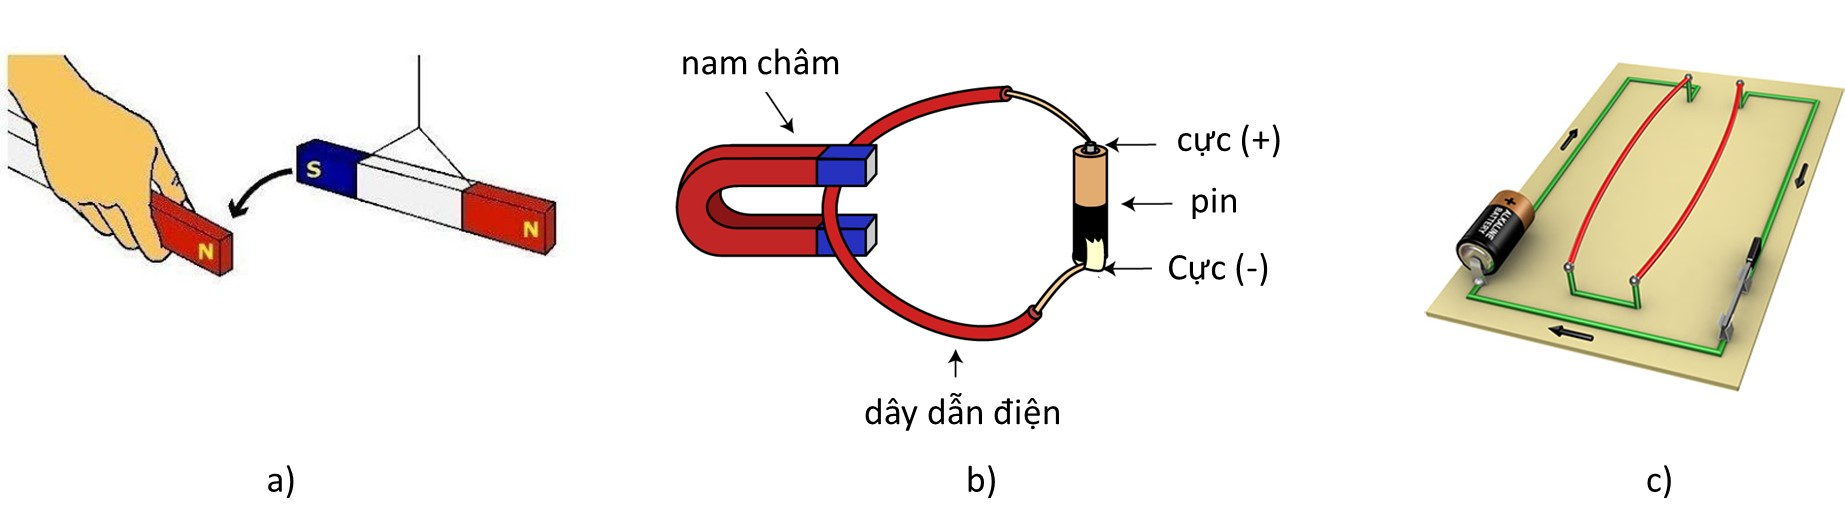
\includegraphics[width=0.9\linewidth]{figs/VN12-Y24-PH-SYL-017-1}
		\captionof{figure}{Tương tác từ giữa a) hai nam châm; b) nam châm với dòng điện; c) dòng điện với dòng điện.}
	\end{center}
	\subsubsection{Từ trường}
	\paragraph{Khái niệm từ trường}
	\begin{dn}
		Từ trường là trường lực gây ra bởi dòng điện hoặc nam châm, là một dạng của vật chất tồn tại xung quanh dòng điện hoặc nam châm mà biểu hiện cụ thể là sự xuất hiện của lực từ tác dụng lên một dòng điện hay một nam châm khác đặt trong nó.
	\end{dn}
	\paragraph{Từ phổ}
	\begin{dn}
		Từ phổ là hình ảnh tạo ra bởi các mạt sắt trong từ trường đang xét. Từ phổ cho thấy hình ảnh trực quan của từ trường.
	\end{dn}
	\begin{center}
		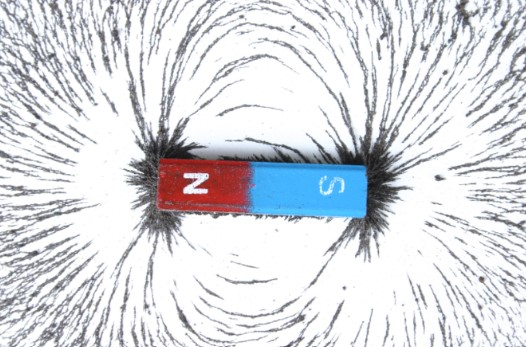
\includegraphics[width=0.4\linewidth]{figs/VN12-Y24-PH-SYL-017-2}
		\captionof{figure}{Từ phổ của một nam châm thẳng.}
	\end{center}
	\subsubsection{Cảm ứng từ}
	\paragraph{Khái niệm cảm ứng từ}
	\begin{dn}
		\begin{itemize}
			\item Để đặc trưng cho từ trường về mặt tác dụng lực, người ta đưa vào một đại lượng vector gọi là cảm ứng từ, kí hiệu là $\vec{B}$. 
			\item Phương của $\vec{B}$ là phương của nam châm thử nằm cân bằng tại một điểm trong từ trường.
			\item Chiều của $\vec{B}$ là chiều từ cực Nam sang Bắc của nam châm thử.
			\item Lực từ tác dụng lên một dòng điện (đoạn dây dẫn có dòng điện chạy qua) hay một nam châm đặt trong từ trường ở điểm nào lớn hơn thì cảm ứng từ tại điểm đó lớn hơn.
		\end{itemize}
	\end{dn}
	
	\paragraph{Đường sức từ}
	\begin{dn}
		Đường sức từ là những đường mô tả từ trường, sao cho tiếp tuyến tại bất kì điểm nào trên đường sức từ đều có phương, chiều trùng với phương, chiều của vector cảm ứng từ tại điểm đó.
	\end{dn}
	\begin{center}
		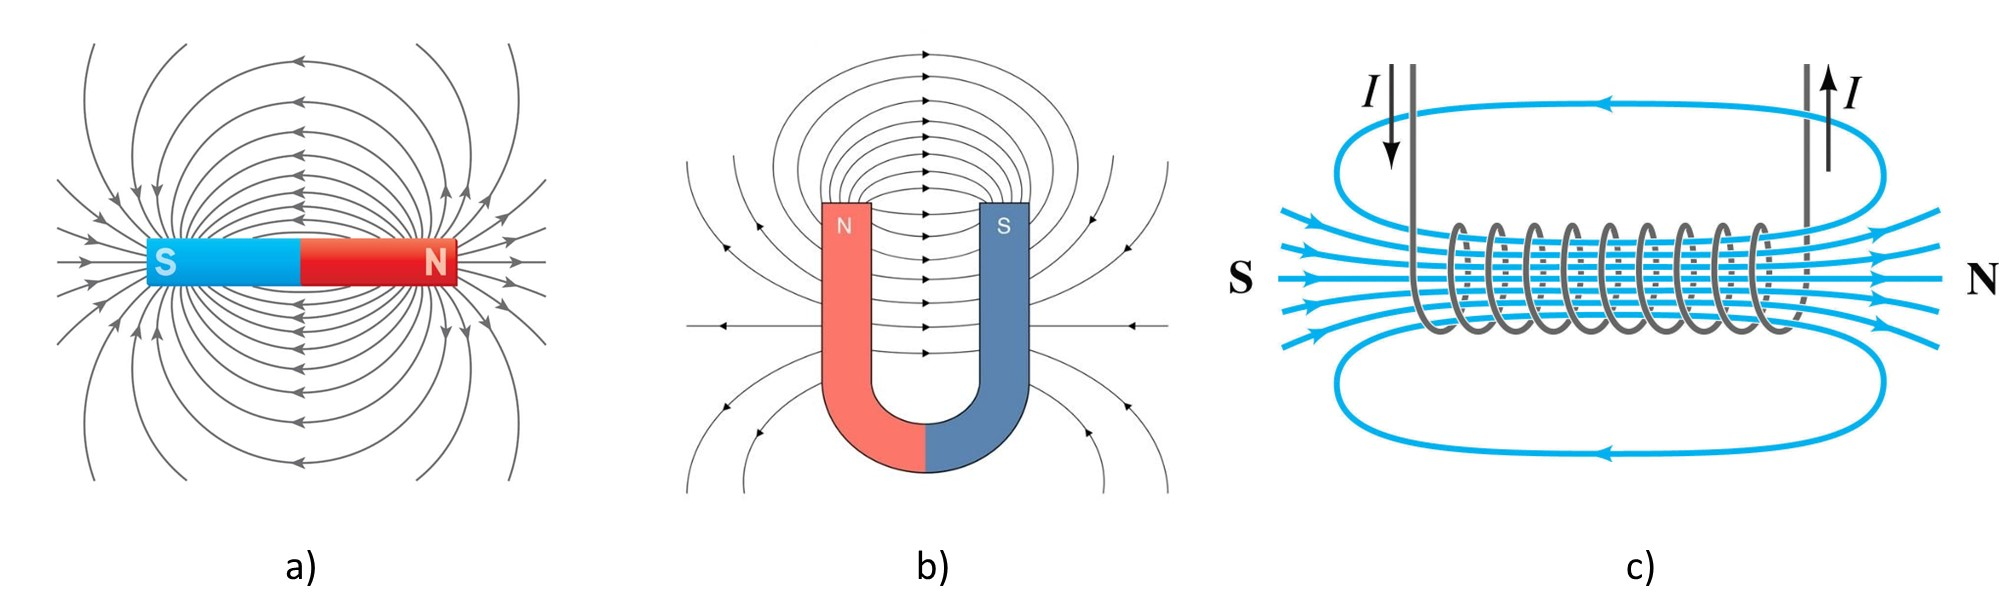
\includegraphics[width=0.85\linewidth]{figs/VN12-Y24-PH-SYL-017-3}
		\captionof{figure}{\textbf{Các đường sức từ của} a) nam châm thẳng; b) nam châm chữ U; c) ống dây có dòng điện chạy qua.}
	\end{center}
	\textbf{Tính chất của các đường sức từ:}
	\begin{tc}
		\begin{itemize}
			\item Tại mỗi điểm trong từ trường, có một và chỉ một đường sức từ đi qua điểm đó.
			\item Các đường sức từ là những đường cong kín. Đối với nam châm, các đường sức từ đi ra từ cực Bắc (N) và đi vào cực Nam (S).
			\item Nơi nào từ trường mạnh hơn thì các đường sức từ ở đó mau (dày) hơn, nơi nào từ trường yếu hơn thì các đường sức từ ở đó thưa hơn.
		\end{itemize}
	\end{tc}
	\paragraph{Từ trường đều}
	\begin{dn}
		Từ trường đều là từ trường có cảm ứng từ $\vec{B}$ tại mọi điểm đều bằng nhau.
	\end{dn}
	\textbf{\textit{Ví dụ:}} Vùng không gian giữa hai cực của nam châm chữ U có các đường sức từ gần như song song và cách đều nhau. Khi đó, từ trường giữa hai cực của nam châm chữ U được gọi là từ trường đều.
	\paragraph{Đường sức từ của một số dây dẫn đặc biệt}
	\begin{itemize}
		\item \textbf{Dòng điện thẳng}\\
		Đường sức từ của dòng điện điện thẳng là những đường tròn đồng tâm với tâm là giao điểm của đoạn dây dẫn và mặt phẳng.
		\begin{center}
			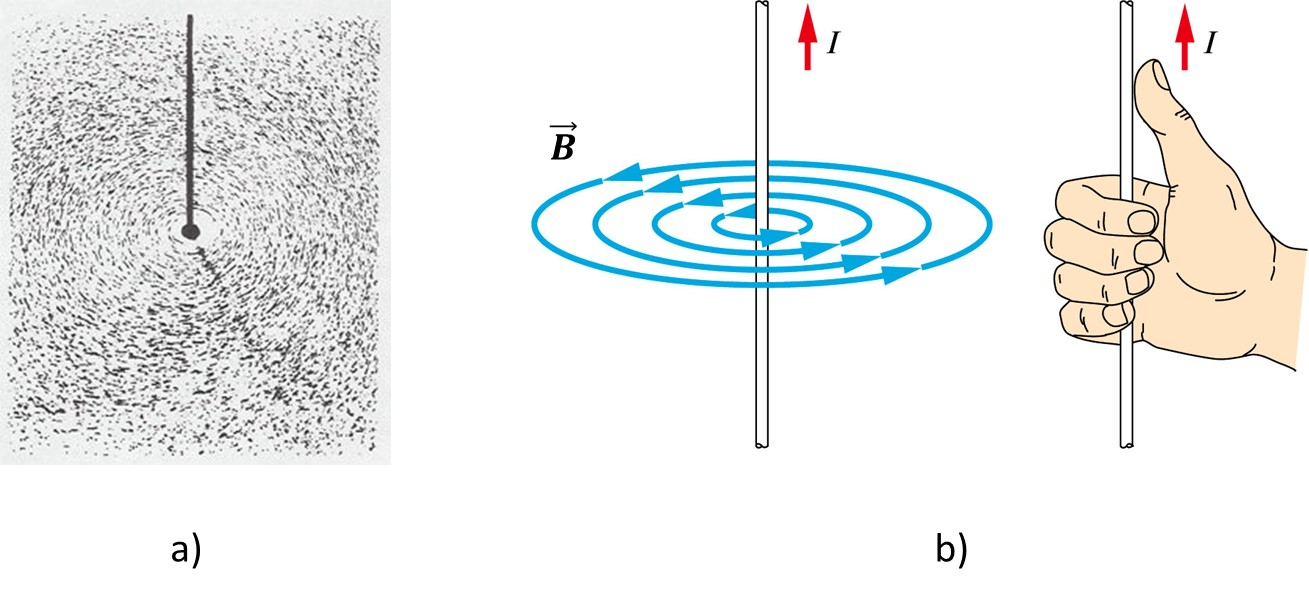
\includegraphics[width=0.6\linewidth]{{figs/VN12-Y24-PH-SYL-017-4}}
			\captionof{figure}{a) Từ phổ của dòng điện thẳng; b) Quy tắc nắm bàn tay phải để xác định chiều đường sức từ của dòng điện thẳng. }
		\end{center}
		\begin{noidung}{Quy tắc bàn tay phải để xác định chiều đường sức từ của dòng điện thẳng}
			Đặt bàn tay phải sao cho ngón cái hướng theo chiều dòng điện, khum các ngón tay còn lại xung quanh đoạn dây dẫn, khi đó chiều từ cổ tay đến các ngón tay chỉ chiều của đường sức từ.
		\end{noidung}
		\item \textbf{Dòng điện tròn}\\
		Đường sức từ tại những điểm nằm trên trục vòng dây của dòng điện tròn là đường thẳng.
		\begin{center}
			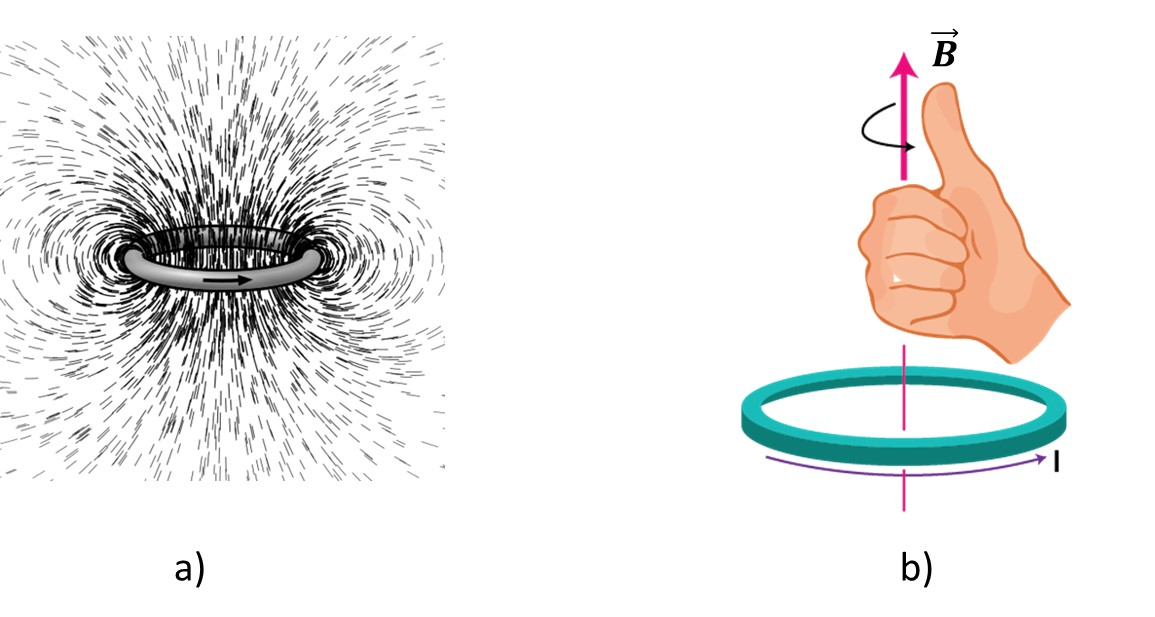
\includegraphics[width=0.6\linewidth]{figs/VN12-Y24-PH-SYL-017-5}
			\captionof{figure}{a) Từ phổ của dòng điện tròn, b) Quy tắc nắm tay phải để xác định chiều đường sức từ trên trục vòng dây của dòng điện tròn.}
		\end{center}
		\begin{noidung}{Quy tắc nắm tay phải để xác định chiều đường sức từ tại tâm của dòng điện tròn}
			Khum bàn tay phải theo vòng dây tròn sao cho chiều từ cổ tay đến các ngón tay trùng với chiều dòng điện trong dây dẫn; khi đó ngón cái choãi ra chỉ chiều của đường sức từ xuyên qua mặt phẳng dòng điện.
		\end{noidung}
		\item \textbf{Dòng điện trong ống dây}\\
		Đường sức từ tại những điểm nằm trên đường đi qua trục của ống dây là đường thẳng. Nếu chiều dài ống dây rất lớn so với bán kính các vòng dây, các đường sức từ bên trong ống dây sẽ song song và cách đều nhau. Một cách gần đúng, ta có thể xem từ trường bên trong ống dây là từ trường đều.
		\begin{center}
			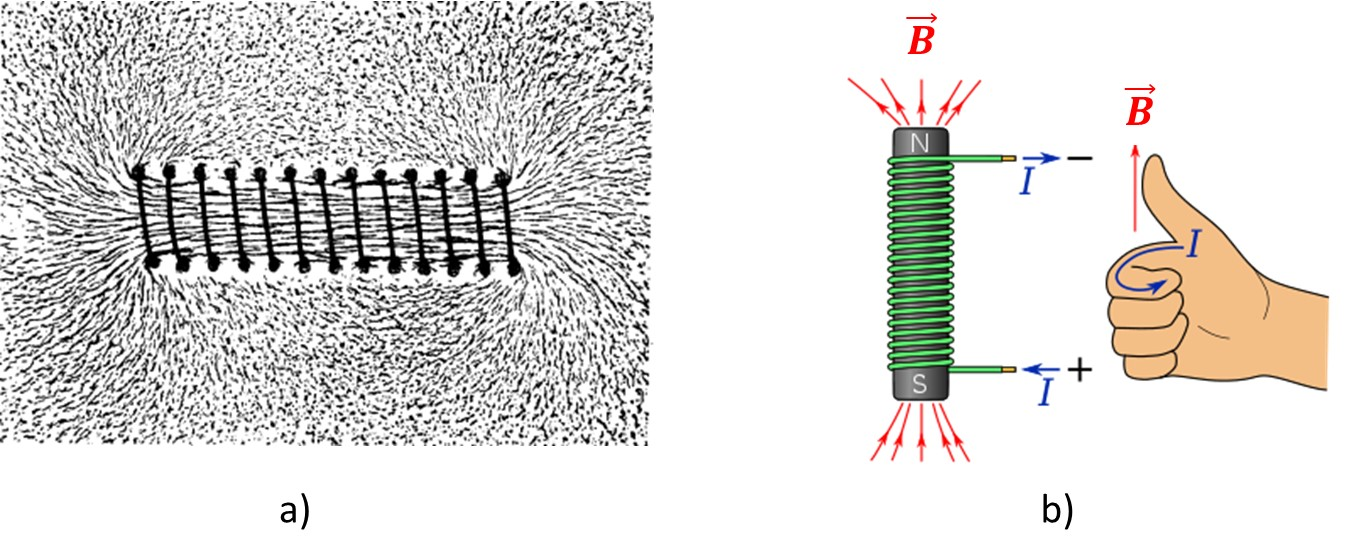
\includegraphics[width=0.6\linewidth]{figs/VN12-Y24-PH-SYL-017-6}
			\captionof{figure}{a) Từ phổ của dòng điện trong ống dây; b) Quy tắc nắm tay phải để xác định chiều của đường sức từ bên trong ống dây.}
		\end{center}
		\begin{noidung}{Quy tắc nắm tay phải để xác định chiều đường sức từ tại tâm của ống dây}
			Tưởng tượng dùng bàn tay phải nắm lấy ống dây sao cho các ngón trỏ, ngón giữa, \dots hướng theo chiều dòng điện; khi đó ngón cái choãi ra chỉ chiều của đường sức từ trong lòng ống dây.
		\end{noidung}
	\end{itemize}
\end{tomtat}
\subsection{Ví dụ minh họa}
\begin{dang}{Nêu được khái niệm từ trường và biểu hiện của từ trường}
\end{dang}
\begin{vd}
	Một học sinh có một nam châm đã biết vị trí cực Bắc và cực Nam. Để có thể sử dụng nam châm này xác định cực Bắc và cực Nam của các nam châm khác, học sinh này sẽ phải làm thế như nào?
	\loigiai{Đưa cực Bắc của nam châm đã biết lại gần một đầu của nam châm chưa xác định cực:
		\begin{itemize}
			\item nếu nam châm bị đẩy thì cực của nam châm chưa biết là cực Bắc.
			\item nếu nam châm bị hút thì cực của nam châm  chưa biết là cực Nam.
	\end{itemize}}
\end{vd}
\begin{vd}
	Đoạn dây dẫn AB căng thẳng mang điện tích. Nếu đưa một nam châm lại gần như hình thì đoạn dây AB có bị tác dụng bởi nam châm hay không? Giải thích.
	\begin{center}
		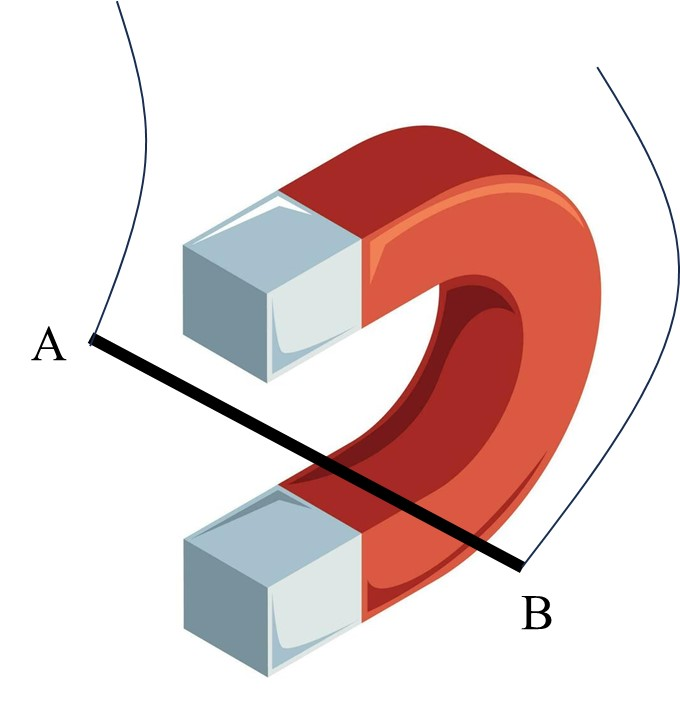
\includegraphics[width=0.25\linewidth]{figs/VN12-Y24-PH-SYL-017-7}
	\end{center}
	\loigiai{
	Đoạn dây AB không bị tác dụng bởi nam châm.\\
	Vì từ trường tác dụng lên dòng điện mà không tác dụng lên điện tích tĩnh.
	}
\end{vd}
\begin{dang}{Vận dụng quy tắc nắm tay phải để xác định chiều đường sức từ hoặc chiều dòng điện}
	\end{dang}
\begin{vd}
	Cho biết hình dạng và chiều của các đường sức từ như các hình vẽ. Xác định chiều của dòng điện chạy trong các dây dẫn ở các trường hợp sau:
	\begin{center}
		\begin{longtable}{M{8cm}M{8cm}}
			\begin{tikzpicture}[>=latex,line width=.7pt]
				\foreach \r in {1,2,3,4} 
				\draw[
				decoration={markings, mark=at position 0.125 with {\arrow{>}}},
				decoration={markings, mark=at position 0.625 with {\arrow{>}}},
				postaction={decorate}
				]
				(0,0) circle (\r/2);
			\end{tikzpicture}&
			\begin{tikzpicture}[>=latex,line width=.7pt]
				\node [cylinder, fill=gray!50, line width=1.5pt, shape border rotate=180, draw, minimum height=6.0cm, minimum width=1.0cm] at (4.5,0) {};
				\foreach \n in {1,2,3}
				\draw[
				decoration={markings, mark=at position 0.5 with {\arrow{>}}}, preaction={draw,white,line width=2pt}, postaction={decorate}
				]  (2*\n,0.5) arc (165:-165:0.5cm and 2cm);
			\end{tikzpicture}\\
			Hình a & Hình b
		\end{longtable}
	\end{center}
	\begin{note}
	Quy ước:
	\begin{itemize}
		\item $\otimes$ chiều dòng điện hướng vuông góc từ ngoài vào trong trang giấy.
		\item $\odot$ chiều dòng điện hướng vuông góc từ trong trang giấy ra ngoài.
	\end{itemize}
		\end{note}
		\loigiai{
		\begin{center}
			\begin{longtable}{M{8cm}M{8cm}}
				\begin{tikzpicture}[>=latex,line width=.7pt]
					\foreach \r in {1,2,3,4} 
					\draw[
					decoration={markings, mark=at position 0.125 with {\arrow{>}}},
					decoration={markings, mark=at position 0.625 with {\arrow{>}}},
					postaction={decorate}
					]
					(0,0) circle (\r/2);
					\draw[blue, line width=1.25pt] (0,0) circle (0.25);
					\filldraw[blue] (0,0) circle (2pt) ;
					\node [blue] at (0,0.65) {$I$};
				\end{tikzpicture}
				&
				\begin{tikzpicture}[>=latex,line width=.7pt]
					\node [cylinder, fill=gray!50, line width=1.5pt, shape border rotate=180, draw, minimum height=6.0cm, minimum width=1.0cm] at (4.5,0) {};
					\foreach \n in {1,2,3}
					\draw[
					decoration={markings, mark=at position 0.5 with {\arrow{>}}}, preaction={draw,white,line width=2pt}, postaction={decorate}
					]  (2*\n,0.5) arc (165:-165:0.5cm and 2cm);
					\draw[line width=1.25pt, blue, -latex] (7.4,0)--(9,0);
					\node[blue, above] at (9,0) {$I$};
				\end{tikzpicture}\\
				Hình a & Hình b
			\end{longtable}
		\end{center}
		}
\end{vd}
\begin{vd}
Hãy xác định cực của ống dây và cực của kim nam châm trong hai hình sau:\\
\begin{center}
	\begin{longtable}{M{8cm}M{8cm}}
		\begin{tikzpicture}		
			\def\coil#1{
				{0.2 * (2*#1 + \t) + 0.4*sin(\t * pi r))},
				{0.65 * cos(\t * pi r)}
			}
			
			% Draw the part of the coil behind the rectangle
			\foreach \n in {1,2,...,10} {
				\draw[domain={0:1},smooth,variable=\t,samples=100]
				plot (\coil{\n}); 
			}
			
			% Draw the cylinder
			\node [cylinder, fill=white, line width=1.5pt, shape border rotate=180, draw, minimum height=5.0cm, minimum width=1.0cm] at (2.15,0) {};
			% Draw the part of the coil in front of the rectangle
			\foreach \n in {0,1,...,9} {
				\draw[domain={1:2},smooth,variable=\t,samples=100,  
				preaction={draw,white,line width=2pt,}     % remove if undesired
				] 
				plot (\coil{\n});
				%	\node[rotate=80] at (-0.05+0.4*\n, 0) {>};
			}
			\draw[line width=0.8pt] (0.20,-0.65)--(0.20,-3)--(4.20,-3)--(4.20,-0.65);
			\node[draw, line width=1pt, fill=white, shape=rectangle, minimum width=1.5cm, minimum height=0.5cm, anchor=center] at (2.22,-3) {};
			\node[above] at (1.5,-2.75) {+};
			\node[above] at (3,-2.75) {-};
			\draw[line width=1pt](-2,-0.25)--(-2,0.25)--(-3,0)--(-2,-0.25);
			\draw[line width=1pt](-2,-0.25)--(-2,0.25)--(-1,0)--(-2,-0.25);
		\end{tikzpicture}
		&
		\begin{tikzpicture}		
			\def\coil#1{
				{0.2 * (2*#1 + \t) + 0.4*sin(\t * pi r))},
				{0.65 * cos(\t * pi r)}
			}
			
			% Draw the part of the coil behind the rectangle
			\foreach \n in {1,2,...,10} {
				\draw[domain={0:1},smooth,variable=\t,samples=100]
				plot (\coil{\n}); 
			}
			
			% Draw the cylinder
			\node [cylinder, fill=white, line width=1.5pt, shape border rotate=180, draw, minimum height=5.0cm, minimum width=1.0cm] at (2.15,0) {};
			% Draw the part of the coil in front of the rectangle
			\foreach \n in {0,1,...,9} {
				\draw[domain={1:2},smooth,variable=\t,samples=100,  
				preaction={draw,white,line width=2pt,}     % remove if undesired
				] 
				plot (\coil{\n});
				%	\node[rotate=80] at (-0.05+0.4*\n, 0) {>};
			}
			\draw[line width=0.8pt] (0.20,-0.65)--(0.20,-3)--(4.20,-3)--(4.20,-0.65);
			\node[draw, line width=1pt, fill=white, shape=rectangle, minimum width=1.5cm, minimum height=0.5cm, anchor=center] at (2.22,-3) {};
			\node[above] at (1.5,-2.75) {-};
			\node[above] at (3,-2.75) {+};
			\draw[line width=1pt](2,-1.5)--(2,-1.0)--(1,-1.25)--(2,-1.5);
			\draw[line width=1pt](2,-1.5)--(2,-1.0)--(3,-1.25)--(2,-1.5);
		\end{tikzpicture}\\
		Hình a & Hình b
	\end{longtable}
\end{center}
\loigiai{
\begin{center}
	\begin{longtable}{M{8cm}M{8cm}}
		\begin{tikzpicture}		
			\def\coil#1{
				{0.2 * (2*#1 + \t) + 0.4*sin(\t * pi r))},
				{0.65 * cos(\t * pi r)}
			}	
			% Draw the part of the coil behind the cylinder
			\foreach \n in {1,2,...,10} {
				\draw[domain={0:1},smooth,variable=\t,samples=100]
				plot (\coil{\n}); 
			}	
			% Draw the cylinder
			\node [cylinder, fill=white, line width=1.5pt, shape border rotate=180, draw, minimum height=5.0cm, minimum width=1.0cm] at (2.15,0) {};
			% Draw the part of the coil in front of the rectangle
			\foreach \n in {0,1,...,9} {
				\draw[domain={1:2},smooth,variable=\t,samples=100,  
				preaction={draw,white,line width=2pt,}     % remove if undesired
				] 
				plot (\coil{\n});
				\node[rotate=80] at (-0.1+0.4*\n, 0) {>};
			}
			\draw[line width=0.8pt] (0.20,-0.65)--(0.20,-3)--(4.20,-3)--(4.20,-0.65);
			\node[draw, line width=1pt, fill=white, shape=rectangle, minimum width=1.5cm, minimum height=0.5cm, anchor=center] at (2.22,-3) {};
			\node[above] at (1.5,-2.75) {+};
			\node[above] at (3,-2.75) {-};
			\draw[line width=1pt,fill=blue!75!black](-2,-0.25)--(-2,0.25)--(-3,0)--(-2,-0.25);
			\draw[line width=1pt](-2,-0.25)--(-2,0.25)--(-1,0)--(-2,-0.25);
		\end{tikzpicture}
		&
		\begin{tikzpicture}		
			
			\def\coil#1{
				{0.2 * (2*#1 + \t) + 0.4*sin(\t * pi r))},
				{0.65 * cos(\t * pi r)}
			}
			
			% Draw the part of the coil behind the rectangle
			\foreach \n in {1,2,...,10} {
				\draw[domain={0:1},smooth,variable=\t,samples=100]
				plot (\coil{\n}); 
			}
			
			% Draw the cylinder
			\node [cylinder, fill=white, line width=1.5pt, shape border rotate=180, draw, minimum height=5.0cm, minimum width=1.0cm] at (2.15,0) {};
			% Draw the part of the coil in front of the rectangle
			\foreach \n in {0,1,...,9} {
				\draw[domain={1:2},smooth,variable=\t,samples=100,  
				preaction={draw,white,line width=2pt,}     % remove if undesired
				] 
				plot (\coil{\n});
				\node[rotate=80] at (-0.1+0.4*\n, 0) {<};
			}
			\draw[line width=0.8pt] (0.20,-0.65)--(0.20,-3)--(4.20,-3)--(4.20,-0.65);
			\node[draw, line width=1pt, fill=white, shape=rectangle, minimum width=1.5cm, minimum height=0.5cm, anchor=center] at (2.22,-3) {};
			\node[above] at (1.5,-2.75) {-};
			\node[above] at (3,-2.75) {+};
			\draw[line width=1pt, fill=blue!75!black](2,-1.5)--(2,-1.0)--(1,-1.25)--(2,-1.5);
			\draw[line width=1pt](2,-1.5)--(2,-1.0)--(3,-1.25)--(2,-1.5);
		\end{tikzpicture}\\
		Hình a & Hình b
	\end{longtable}
\end{center}
}
\end{vd}

\begin{vd}
Hãy xác định cực của nguồn AB trong hai trường hợp sau:\\
\begin{center}
	\begin{longtable}{M{8cm}M{8cm}}
		\begin{tikzpicture}		
			\def\coil#1{
				{0.2 * (2*#1 + \t) + 0.4*sin(\t * pi r))},
				{0.65 * cos(\t * pi r)}
			}
			
			% Draw the part of the coil behind the rectangle
			\foreach \n in {1,2,...,10} {
				\draw[domain={0:1},smooth,variable=\t,samples=100]
				plot (\coil{\n}); 
			}
			
			% Draw the cylinder
			\node [cylinder, fill=white, line width=1.5pt, shape border rotate=180, draw, minimum height=5.0cm, minimum width=1.0cm] at (2.15,0) {};
			% Draw the part of the coil in front of the rectangle
			\foreach \n in {0,1,...,9} {
				\draw[domain={1:2},smooth,variable=\t,samples=100,  
				preaction={draw,white,line width=2pt,}     % remove if undesired
				] 
				plot (\coil{\n});
				%\node[rotate=70] at (-0.08+0.4*\n, 0) {<};
			}
			\draw[line width=0.8pt] (0.20,-0.65)--(0.20,-3)--(4.20,-3)--(4.20,-0.65);
			\node[draw, line width=1pt, fill=white, shape=rectangle, minimum width=1.5cm, minimum height=0.5cm, anchor=center] at (2.22,-3) {};
			\draw[line width=1pt, fill=blue!75!black](2,1)--(2,1.5)--(1,1.25)--(2,1);
			\draw[line width=1pt](2,1)--(2,1.5)--(3,1.25)--(2,1);
			\node[below] at (1.5,-3.25) {A};
			\node[below] at (3,-3.25) {B};
		\end{tikzpicture}
		&
		\begin{tikzpicture}		
			\def\coil#1{
				{0.2 * (2*#1 + \t) + 0.4*sin(\t * pi r))},
				{0.65 * cos(\t * pi r)}
			}
			
			% Draw the part of the coil behind the rectangle
			\foreach \n in {1,2,...,10} {
				\draw[domain={0:1},smooth,variable=\t,samples=100]
				plot (\coil{\n}); 
			}
			
			% Draw the cylinder
			\node [cylinder, fill=white, line width=1.5pt, shape border rotate=180, draw, minimum height=5.0cm, minimum width=1.0cm] at (2.15,0) {};
			% Draw the part of the coil in front of the rectangle
			\foreach \n in {0,1,...,9} {
				\draw[domain={1:2},smooth,variable=\t,samples=100,  
				preaction={draw,white,line width=2pt,}     % remove if undesired
				] 
				plot (\coil{\n});
				%	\node[rotate=70] at (-0.08+0.4*\n, 0) {<};
			}
			\draw[line width=0.8pt] (0.20,-0.65)--(0.20,-3)--(4.20,-3)--(4.20,-0.65);
			\node[draw, line width=1pt, fill=white, shape=rectangle, minimum width=1.5cm, minimum height=0.5cm, anchor=center] at (2.22,-3) {};
			\draw[line width=1pt](6,-0.25)--(6,0.25)--(5,0)--(6,-0.25);
			\draw[line width=1pt, fill=blue!75!black](6,-0.25)--(6,0.25)--(7,0)--(6,-0.25);
			\node[below] at (1.5,-3.25) {A};
			\node[below] at (3,-3.25) {B};
		\end{tikzpicture}\\
		Hình a & Hình b
	\end{longtable}
\end{center}
\loigiai{
	\begin{center}
		\begin{longtable}{M{8cm}M{8cm}}
			\begin{tikzpicture}	
				\def\coil#1{
					{0.2 * (2*#1 + \t) + 0.4*sin(\t * pi r))},
					{0.65 * cos(\t * pi r)}
				}
				
				% Draw the part of the coil behind the rectangle
				\foreach \n in {1,2,...,10} {
					\draw[domain={0:1},smooth,variable=\t,samples=100]
					plot (\coil{\n}); 
				}
				
				% Draw the cylinder
				\node [cylinder, fill=white, line width=1.5pt, shape border rotate=180, draw, minimum height=5.0cm, minimum width=1.0cm] at (2.15,0) {};
				% Draw the part of the coil in front of the rectangle
				\foreach \n in {0,1,...,9} {
					\draw[domain={1:2},smooth,variable=\t,samples=100,  
					preaction={draw,white,line width=2pt,}     % remove if undesired
					] 
					plot (\coil{\n});
					\node[rotate=80] at (-0.1+0.4*\n, 0) {<};
				}
				\draw[line width=0.8pt] (0.20,-0.65)--(0.20,-3)--(4.20,-3)--(4.20,-0.65);
				\node[draw, line width=1pt, fill=white, shape=rectangle, minimum width=1.5cm, minimum height=0.5cm, anchor=center] at (2.22,-3) {};
				\node[above] at (1.5,-2.75) {-};
				\node[above] at (3,-2.75) {+};
				\node[below] at (1.5,-3.25) {A};
				\node[below] at (3,-3.25) {B};
				\node[right,red] at (4.5,0) {N};
				\node[left,red] at (-0.4,0) {S};
				\draw[line width=1pt, fill=blue!75!black](2,1)--(2,1.5)--(1,1.25)--(2,1);
				\draw[line width=1pt](2,1)--(2,1.5)--(3,1.25)--(2,1);
			\end{tikzpicture}
			&
			\begin{tikzpicture}		
				\def\coil#1{
					{0.2 * (2*#1 + \t) + 0.4*sin(\t * pi r))},
					{0.65 * cos(\t * pi r)}
				}
				
				% Draw the part of the coil behind the rectangle
				\foreach \n in {1,2,...,10} {
					\draw[domain={0:1},smooth,variable=\t,samples=100]
					plot (\coil{\n}); 
				}
				
				% Draw the cylinder
				\node [cylinder, fill=white, line width=1.5pt, shape border rotate=180, draw, minimum height=5.0cm, minimum width=1.0cm] at (2.15,0) {};
				% Draw the part of the coil in front of the rectangle
				\foreach \n in {0,1,...,9} {
					\draw[domain={1:2},smooth,variable=\t,samples=100,  
					preaction={draw,white,line width=2pt,}     % remove if undesired
					] 
					plot (\coil{\n});
					\node[rotate=80] at (-0.1+0.4*\n, 0) {<};
				}
				
				\draw[line width=0.8pt] (0.20,-0.65)--(0.20,-3)--(4.20,-3)--(4.20,-0.65);
				\node[draw, line width=1pt, fill=white, shape=rectangle, minimum width=1.5cm, minimum height=0.5cm, anchor=center] at (2.22,-3) {};
				\node[above] at (1.5,-2.75) {-};
				\node[above] at (3,-2.75) {+};
				\node[below] at (1.5,-3.25) {A};
				\node[below] at (3,-3.25) {B};
				\node[right,red] at (4.5,0) {N};
				\node[left,red] at (-0.4,0) {S};
				\draw[line width=1pt](6,-0.25)--(6,0.25)--(5,0)--(6,-0.25);
				\draw[line width=1pt, fill=blue!75!black](6,-0.25)--(6,0.25)--(7,0)--(6,-0.25);
			\end{tikzpicture}\\
			Hình a & Hình b
		\end{longtable}
	\end{center}
}
\end{vd}
\subsection{Bài tập}
\subsubsection{Trắc nghiệm nhiều phương án lựa chọn}
\setcounter{ex}{0}
\Opensolutionfile{ans}[ans/VN12-Y24-PH-SYL-017P-TN]
% ===================================================================
\begin{ex}
	Một thanh nam châm bao giờ cũng có
	\choice
	{một loại cực từ}
	{\True hai loại cực từ}
	{ba loại cực từ}
	{một hoặc hai loại cực từ}
	\loigiai{}
\end{ex}
% ===================================================================
\begin{ex}
	Khi đưa cực từ bắc của thanh nam châm này lại gần cực từ nam của thanh nam châm kia thì
	\choice
	{\True chúng hút nhau}
	{tạo ra dòng điện}
	{chúng đẩy nhau}
	{chúng không hút nhau cũng không đẩy nhau}
	\loigiai{}
\end{ex}
% ===================================================================
\begin{ex}
	Sự sắp xếp kim nam châm ở hình nào sau đây là \textbf{đúng}?	
	\begin{center}
		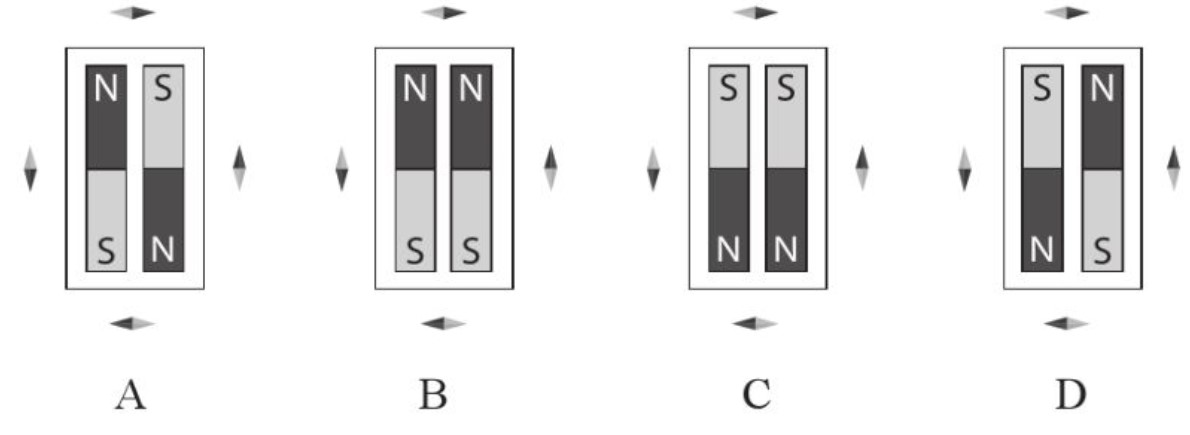
\includegraphics[width=0.7\linewidth]{figs/VN12-Y24-PH-SYL-017P-7}
	\end{center}
	\choice
	{\True A}
	{B}
	{C}
	{D}
	\loigiai{}
\end{ex}

% ===================================================================
\begin{ex}
	Tương tác từ \textbf{không} xảy ra trong trường hợp nào sau đây?
	\choice
	{Một thanh nam châm và một dòng điện không đổi đặt gần nhau}
	{Hai thanh nam châm đặt gần nhau}
	{\True Một thanh nam châm và một thanh đồng đặt gần nhau}
	{Một thanh nam châm và một thanh sắt non đặt gần nhau}
	\loigiai{}
\end{ex}
% ===================================================================
\begin{ex}
	Tính chất cơ bản của từ trường là
	\choice
	{\True gây ra lực từ tác dụng lên nam châm hoặc lên dòng điện đặt trong đó}
	{gây ra lực hấp dẫn lên các vật đặt trong đó}
	{gây ra lực đàn hồi tác dụng lên các dòng điện và nam châm đặt trong đó}
	{gây ra sự biến đổi về tính chất điện của môi trường xung quanh}
	\loigiai{}
\end{ex}
% ===================================================================
\begin{ex}
	Các đường sức từ	
	\choice
	{luôn cắt nhau}
	{\True không bao giờ cắt nhau}
	{luôn song song nhau}
	{có thể cắt nhau hoặc không}
	\loigiai{}
\end{ex}

% ===================================================================
\begin{ex}
	Xung quanh vật nào sau đây \textbf{không} có từ trường?	
	\choice
	{Dòng điện không đổi}
	{Hạt mang điện chuyển động}
	{\True Hạt mang điện đứng yên}
	{Nam châm hình chữ U}
	\loigiai{}
\end{ex}
% ===================================================================
\begin{ex}
	Trong các phát biểu sau, có bao nhiêu phát biểu \textbf{đúng}?	
	\begin{enumerate}[label=(\arabic*)]
		\item Mọi nam châm đều có hai cực: cực âm Nam (S) và cực Bắc  (N).
		\item Một số loài vật có thể sử dụng từ trường để tạo ra dòng điện làm tê liệt con mồi.
		\item Trái Đất là một nam châm khổng lồ, cực Bắc nam châm Trái Đất chính là cực Bắc địa lí và ngược lại.
		\item Cảm ứng từ là đại lượng đặc trưng cho từ trường về mặt năng lượng.
	\end{enumerate}
	\choice
	{\True 1}
	{2}
	{3}
	{4}
	\loigiai{Phát biểu đúng là (1).}
\end{ex}
% ===================================================================
\begin{ex}
	Chỉ ra câu \textbf{sai}.	
	\choice
	{Các đường mạt sắt của từ phổ cho biết dạng của đường sức từ}
	{Các đường sức từ của từ trường đều là những đường thẳng song song, cách đều nhau}
	{Nói chung các đường sức điện của điện tích đứng yên thì không kín, còn các đường sức từ là những đường cong kín}
	{\True Một hạt mang điện chuyển động theo quỹ đạo tròn trong từ trường thì quỹ đạo của nó là một đường sức từ của từ trường}
	\loigiai{}
\end{ex}
% ===================================================================
\begin{ex}
	Các đường sức từ xung quanh dây dẫn thẳng có dòng điện không đổi chạy qua có dạng là	
	\choice
	{những đường thẳng song song với dòng điện}
	{những đường thẳng vuông góc với dòng điện}
	{\True những vòng tròn đồng tâm với tâm nằm tại vị trí nơi dòng điện chạy qua}
	{những đường xoắn ốc đồng trục với trục là dòng điện}
	\loigiai{}
\end{ex}
% ===================================================================
\begin{ex}
	Từ phổ là
	\choice
	{\True hình ảnh của các đường mạt sắt cho ta hình ảnh của các đường sức từ của từ trường}
	{hình ảnh tương tác của hai nam châm với nhau}
	{hình ảnh tương tác giữa dòng điện và nam châm}
	{hình ảnh tương tác của hai dòng điện chạy trong hai dây dẫn thẳng song song}
	\loigiai{}
\end{ex}
% ===================================================================
\begin{ex}
	Phát biểu nào sau đây \textbf{không đúng}?	
	\choice
	{Qua bất kì điểm nào trong từ trường, ta cũng có thể vẽ được một đường sức từ}
	{\True Đường sức từ do nam châm thẳng tạo ra xung quanh nó là những đường thẳng}
	{Đường sức từ mau hơn ở nơi có từ trường lớn hơn, đường sức thưa hơn ở nơi có từ trường nhỏ hơn}
	{Các đường sức từ là những đường cong kín}
	\loigiai{}
\end{ex}
% ===================================================================
\begin{ex}
	Đặt một kim nam châm song song với dòng điện. Khi cho dòng điện chạy qua dây dẫn, ta thấy
	\choice
	{\True kim nam châm lệch một góc so với phương ban đầu}
	{kim nam châm đứng yên}
	{kim nam châm quay tròn xung quanh trục}
	{kim nam châm quay trái, quay phải liên tục}
	\loigiai{}
\end{ex}
% ===================================================================
\begin{ex}
	Phát biểu nào sau đây nói lên tính chất khác biệt của nam châm điện so với nam châm vĩnh cửu?
	\choice
	{Nam châm điện có cực từ bắc và cực từ nam}
	{Nam châm điện có thể hút các vật làm bằng vật liệu sắt từ}
	{\True Có thể bật hoặc tắt từ trường của nam châm điện}
	{Không thể đảo ngược được cực từ của nam châm điện}
	\loigiai{}
\end{ex}
% ===================================================================
\begin{ex}
	Một kim nam châm nhỏ nằm cân bằng tại một điểm trong từ trường. Hướng của từ trường tại điểm đó được quy ước là hướng	
	\choice
	{từ địa cực Bắc sang địa cực Nam của Trái Đất}
	{từ địa cực Nam sang địa cực Bắc của Trái Đất}
	{\True từ cực Nam sang cực Bắc của kim nam châm nhỏ}
	{từ cực Bắc sang cực Nam của kim nam châm nhỏ}
	\loigiai{}
\end{ex}


% ===================================================================
\begin{ex}
	Có hai thanh kim loại bằng sắt, bề ngoài giống nhau. Khi đặt chúng gần nhau thì chúng hút nhau. Kết luận nào sau đây về hai thanh đó là \textbf{đúng}?
	\choice
	{Đó là hai thanh nam châm}
	{Một thanh là nam châm, thanh còn lại là thanh sắt}
	{Có thể là hai thanh nam châm, cũng có thể là hai thanh sắt}
	{\True Có thể là hai thanh nam châm, cũng có thể là một thanh nam châm và một thanh sắt}
	\loigiai{}
\end{ex}
% ===================================================================
\begin{ex}
	Từ trường của một nam châm thẳng giống từ trường được tạo bởi
	\choice
	{một dây dẫn thẳng có dòng điện chạy qua}
	{\True một ống dây có dòng điện chạy qua}
	{một nam châm hình chữ U}
	{một vòng dây tròn có dòng điện chạy qua}
	\loigiai{}
\end{ex}
% ===================================================================
\begin{ex}
	Chọn ý \textbf{sai}. Người ta thường dùng nam châm điện thay cho nam châm vĩnh cửu là do
	\choice
	{nam châm điện có thể tạo ra từ trường mạnh/yếu tuỳ theo nhu cầu sử dụng}
	{nam châm vĩnh cửu tạo ra từ trường không đủ mạnh}
	{nam châm điện có thể thay đổi các cực của nam châm dễ dàng}
	{\True không thể dùng nam châm vĩnh cửu trong các ứng dụng hàng ngày}
	\loigiai{}
\end{ex}
% ===================================================================
\begin{ex}
	Một thanh nam châm được tách làm hai nửa. Chọn phát biểu \textbf{đúng}?
	\choice
	{Từ trường của mỗi mảnh rời nhau trở nên mạnh hơn}
	{Các cực từ được tách ra}
	{\True Hai thanh nam châm mới được tạo ra}
	{Điện trường được sinh ra}
	\loigiai{}
\end{ex}

% ===================================================================
\begin{ex}
	\immini{Cho một dòng điện thẳng, dài, đi qua một tấm bìa như hình vẽ bên. Dòng điện trong dây gây ra một từ trường xung quanh nó. Hình vẽ nào trong hình \ref{fig:17P-8} biểu diễn \textbf{đúng} chiều của các đường sức từ khi nhìn từ phía trên xuống?}
	{
		\begin{tikzpicture}[scale=0.5]
			\coordinate (O) at (0,0);
			\coordinate (A) at ($(O)+(45:3)$);
			\coordinate (C) at (4,0);
			\coordinate (B) at ($(C)+(45:3)$);
			\fill[orange!50!white, opacity=0.6] (O)--(A)--(B)--(C)--(O);
			\draw[line width=1.5pt, blue,decoration={markings, mark=at position 0.625 with {\arrowreversed{stealth}}},
			postaction={decorate}] 
			(3,1.45)--+(0,2);
			
			\draw[line width=1.5pt, blue] (3,0)--+(0,-1);
			\node[right] at (3,3) {$I$};
		\end{tikzpicture}
		%		\caption{}
		%		\label{fig:17P-7}
		
	}
	
	\begin{center}
		\begin{tabular}{cccc}
			\begin{tikzpicture}
				\coordinate (O) at (0,0);
				\foreach \i in {0, 45, ...,315}{
					\draw[line width=1pt, decoration={markings, mark=at position 0.5 with {\arrowreversed{stealth}}},
					postaction={decorate}] (O)--+(\i:2);}
				\node[circle, blue, fill=white, inner sep=0pt, minimum size=0pt] at (O) {$\LARGE\otimes$};
			\end{tikzpicture}
			
			&
			\begin{tikzpicture}
				\coordinate (O) at (0,0);
				\foreach \r in {1,2,3} {
					\draw[line width=1pt, decoration={markings, mark=at position 0 with {\arrow{stealth}}},
					postaction={decorate}
					]
					(0,0) circle (\r/2);	
				}
				\node[circle, blue, fill=white, inner sep=0pt, minimum size=0pt] at (O) {$\LARGE\otimes$};
			\end{tikzpicture}
			&
			\begin{tikzpicture}
				\coordinate (O) at (0,0);
				\foreach \i in {0, 45, ...,315}{
					\draw[line width=1pt, decoration={markings, mark=at position 0.625 with {\arrow{stealth}}},
					postaction={decorate}] (O)--+(\i:2);}
				\node[circle, blue, fill=white, inner sep=0pt, minimum size=0pt] at (O) {$\LARGE\otimes$};
			\end{tikzpicture}
			&
			\begin{tikzpicture}
				\coordinate (O) at (0,0);
				\foreach \r in {1,2,3} {
					\draw[line width=1pt, decoration={markings, mark=at position 0 with {\arrowreversed{stealth}}},
					postaction={decorate}
					]
					(0,0) circle (\r/2);	
				}
				\node[circle, blue, fill=white, inner sep=0pt, minimum size=0pt] at (O) {$\LARGE\otimes$};
			\end{tikzpicture}\\
			Hình a & Hình b & Hình c & Hình d
		\end{tabular}
		\captionof{figure}{}
		\label{fig:17P-8}
	\end{center}
	\choice
	{Hình a}
	{Hình b}
	{Hình c}
	{\True Hình d}
	\loigiai{}
\end{ex}
\Closesolutionfile{ans}

\subsubsection{Trắc nghiệm đúng/sai}
\Opensolutionfile{ans}[ans/VN12-Y24-PH-SYL-017P-TF]
\setcounter{ex}{0}
% ===================================================================
\begin{ex}
	Nhận xét nào sau đây là \textbf{không đúng} khi nói về tương tác từ giữa các vật?
	\choiceTF[t]
	{\True Dòng điện có thể tác dụng lực từ lên nam châm}
	{Nam châm thẳng không thể tác dụng lực từ lên nam châm chữ U}
	{\True Hai dòng diện có thể tương tác từ với nhau}
	{Hai dòng điện ngược chiều không thể tương tác với nhau}
	\loigiai{}
\end{ex}

% ===================================================================
\begin{ex}
	Cho hai nam châm thẳng đặt gần nhau và đối nhau:
	\choiceTF[t]
	{\True Nếu cực Bắc của một nam châm đối diện với cực Nam của nam châm kia, chúng sẽ hút nhau}
	{Nếu hai cực cùng cực đối diện, đường sức từ sẽ đi ra từ một nam châm và kết thúc ở nam châm kia}
	{\True Nếu hai cực Bắc của hai nam châm đặt đối diện nhau, các đường sức từ sẽ đẩy lẫn nhau tạo thành một khu vực không có đường sức từ giữa chúng}
	{Đưa hai cực của nam châm ra xa nhau, lực từ tương tác giữa chúng sẽ mạnh hơn so với khi chúng đặt gần nhau}
	\loigiai{}
\end{ex}
\begin{ex}
	Hình bên biểu diễn đường sức từ của hai nam châm thẳng đặt gần nhau. Từ hình cho biết:
	\begin{center}
		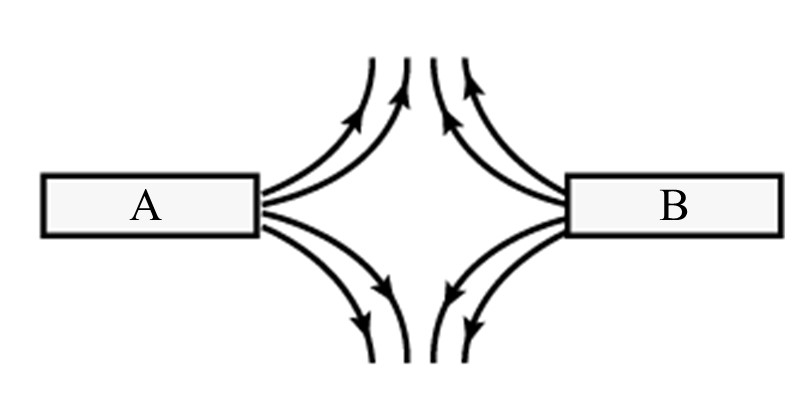
\includegraphics[width=0.35\linewidth]{figs/VN12-Y24-PH-SYL-017P-9}
	\end{center}
	\choiceTF[t]
	{Các cực Nam (S) hướng đối diện nhau}
	{Đường sức từ sẽ xuất phát từ điểm có từ trường mạnh nhất và kết thúc ở điểm có từ trường yếu nhất}
	{\True Khi hai nam châm cùng cực đặt đối diện nhau, đường sức từ sẽ bị biến dạng bởi vì sự tương tác giữa hai từ trường sẽ làm cho các đường sức từ bị uốn cong và hướng ra xa nhau}
	{Nếu các cực cùng tên của hai nam châm đặt đối diện nhau nhưng không chạm, ta có thể quan sát thấy một số đường sức từ chạm vào nhau tại điểm giữa hai nam châm}
	\loigiai{
		\begin{itemchoice}
			\itemch Các cực hướng đối diện nhau trong hình là cực Bắc.
			\itemch Các đường sức từ là các đường cong kín, không có điểm khởi đầu và kết thúc.
			\itemch Đúng.
			\itemch Các đường sức từ không cắt nhau.
		\end{itemchoice}
	}
	
\end{ex}
\Closesolutionfile{ans}
\subsubsection{Tự luận}
\setcounter{ex}{0}
\Opensolutionfile{ans}[ans/VN12-Y24-PH-SYL-017P-TL]
\begin{ex}
	Vẽ chiều của các đường sức từ tương ứng với nam châm thẳng, nam châm chữ U và dòng điện thẳng dài vô hạn trong các hình bên.
	\begin{center}
		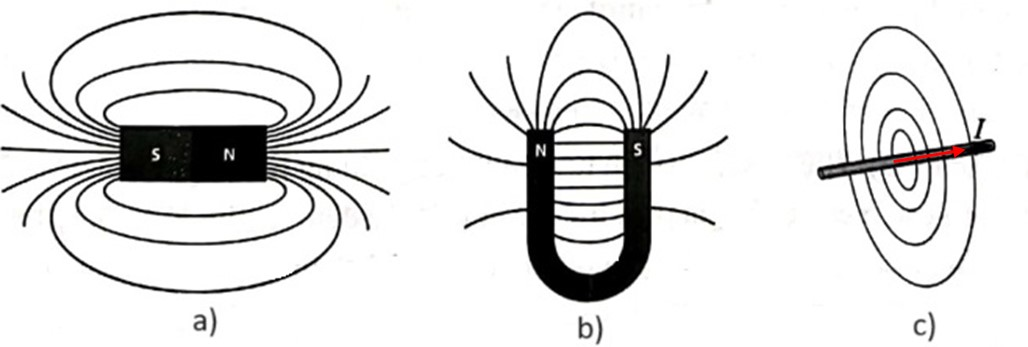
\includegraphics[width=0.8\linewidth]{figs/VN12-Y24-PH-SYL-017P-1}
	\end{center}
	\loigiai{
		\begin{center}
			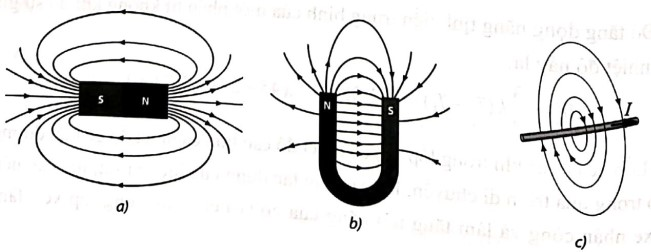
\includegraphics[width=0.6\linewidth]{figs/VN12-Y24-PH-SYL-017P-6}
		\end{center}
	}
\end{ex}

% ===================================================================
\begin{ex}
	Một cuộn dây dẫn được quấn quanh một lõi thép với hai đầu dây nối với nguồn điện không đổi như hình \ref{fig:17P-2}. Hãy vẽ chiều dòng điện trong mạch và vẽ phác các đường sức từ tạo bởi cuộn dây.
	\begin{center}
		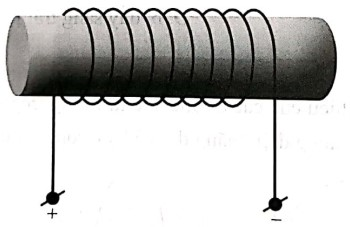
\includegraphics[width=0.3\linewidth]{figs/VN12-Y24-PH-SYL-017P-2}
		\captionof{figure}{}
		\label{fig:17P-2}
	\end{center}
	\loigiai{Chiều dòng điện trong mạch được thể hiện như hình bên. Dựa vào quy tắc nắm tay phải, ta xác định được chiều các đường sức từ tạo bởi ống dây.
		\begin{center}
			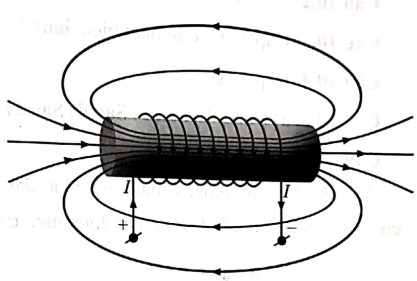
\includegraphics[width=0.4\linewidth]{figs/VN12-Y24-PH-SYL-017P-3}
	\end{center}}
\end{ex}
% ===================================================================
\begin{ex}
	Hiện nay, tàu đệm từ là một trong những phương tiện di chuyển với tốc độ cao ở các quốc gia phát triển. Xét một tàu đệm từ như hình \ref{fig:17P-4}, trong đó tàu được nâng lơ lửng trong không khí bằng hệ thống các nam châm điện. Ngoài ra, trên thân tàu và đường ray còn được gắn các nam châm điện khác đóng vai trò tăng tốc và giảm tốc cho tàu trong quá trình chuyển động.
	\begin{center}
		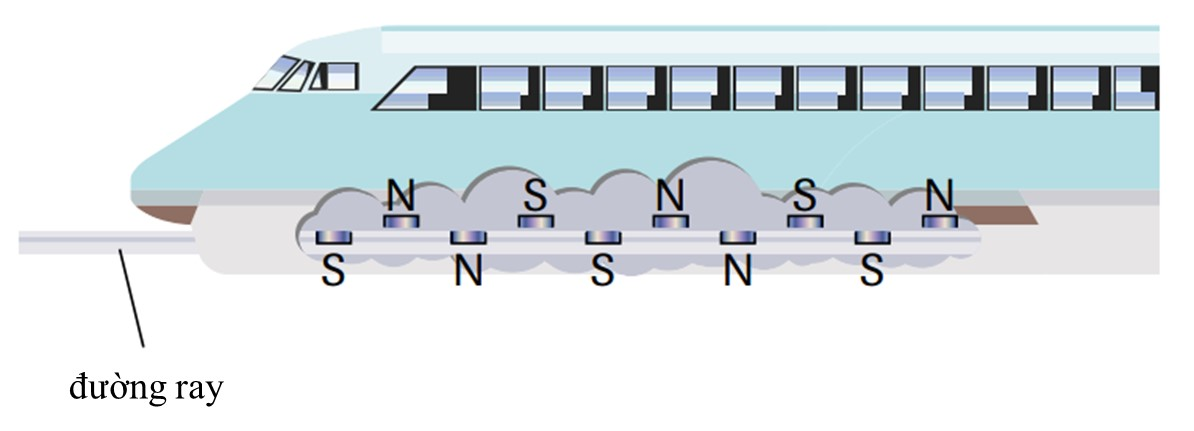
\includegraphics[width=0.6\linewidth]{figs/VN12-Y24-PH-SYL-017P-4}
		\captionof{figure}{}
		\label{fig:17P-4}
	\end{center}	
	\begin{enumerate}[label=\alph*)]
		\item Giả sử tại một thời điểm nào đó, cực từ của các nam châm được mô tả như trong hình, khi đó lực từ tổng hợp tác dụng lên tàu đệm từ đóng vai trò là lực đẩy hay lực cản chuyển động của tàu? Vì sao?
		\item Khi tàu sắp đến nhà ga và bắt đầu chuyển động chậm lại, khi đó chiều dòng điện chạy qua các nam châm điện cần thay đổi như thế nào?
	\end{enumerate}
	\loigiai{
		\begin{enumerate}[label=\alph*)]
			\item Xét bộ 3 nam châm liên tiếp nhau như hình bên. Sự tương tác giữa các cặp nam châm diễn ra như sau:
			\begin{center}
				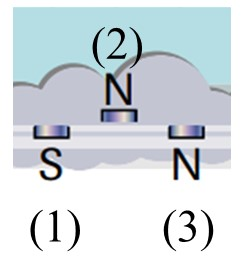
\includegraphics[width=0.15\linewidth]{figs/VN12-Y24-PH-SYL-017P-5}
			\end{center}
			\begin{itemize}
				\item Nam châm (1) hút nam chậm (2).
				\item Nam châm (3) đẩy nam châm (2).
			\end{itemize}
			Kết quả làm tàu đệm từ bị đẩy về phía trước. Điều tương tự xảy ra cho các bộ 3 nam châm liên tiếp nhau còn lại. Do đó, lực từ lúc này đóng vai trò là lực đẩy.
			\item Để tàu đệm từ giảm tốc độ, lực từ phải đóng vai trò là lực cản. Muốn vậy, dòng điện chạy qua bộ 3 nam châm điện liên tiếp nhau trong hình vẽ trên phải đổi chiều sao cho: nam châm (1) đẩy nam châm (2); nam châm (3) hút nam châm (2).
		\end{enumerate}	
	}
\end{ex}
% ===================================================================
\begin{ex}
	Hãy xác định cực của các kim nam châm trong hình \ref{fig:17P-6}.\\
	\begin{center}
		\begin{tabular}{ccc}
			\begin{tikzpicture}[scale=0.75]		
				
				\def\coil#1{
					{0.2 * (2*#1 + \t) + 0.4*sin(\t * pi r))},
					{0.65 * cos(\t * pi r - pi r)}
				}
				
				% Draw the part of the coil behind the rectangle
				\foreach \n in {0,1,2,...,9} {
					\draw[domain={0:1},smooth,variable=\t,samples=100]
					plot (\coil{\n}); 
				}
				
				% Draw the cylinder
				\node [cylinder, fill=white, line width=1.5pt, shape border rotate=180, draw, minimum height=5.0cm, minimum width=1.0cm, scale=0.75] at (2.15,0) {};
				% Draw the part of the coil in front of the rectangle
				\foreach \n in {0,1,...,9} {
					\draw[domain={1:2},smooth,variable=\t,samples=100,  
					preaction={draw,white,line width=2pt,}     % remove if undesired
					] 
					plot (\coil{\n});
					%	\node[rotate=80] at (-0.05+0.4*\n, 0) {>};
				}
				\draw[line width=0.8pt] (0,-0.65)--(0,-3)--(4,-3)--(4,-0.65);
				\node[draw, line width=1pt, fill=white, shape=rectangle, minimum width=1.5cm, minimum height=0.5cm, anchor=center] at (2.22,-3) {};
				\node[above] at (1.5,-2.75) {+};
				\node[above] at (3,-2.75) {-};
				\draw[line width=1pt](-2,-0.25)--(-2,0.25)--(-3,0)--(-2,-0.25);
				\draw[line width=1pt](-2,-0.25)--(-2,0.25)--(-1,0)--(-2,-0.25);
				\node[below] at (2,-3.5) {a)};
			\end{tikzpicture}
			&
			\begin{tikzpicture}[scale=0.75]		
				\def\coil#1{
					{0.2 * (2*#1 + \t) + 0.4*sin(\t * pi r))},
					{0.65 * cos(\t * pi r - pi r)}
				}
				
				% Draw the part of the coil behind the rectangle
				\foreach \n in {0,1,2,...,9} {
					\draw[domain={0:1},smooth,variable=\t,samples=100]
					plot (\coil{\n}); 
				}
				
				% Draw the cylinder
				\node [cylinder, fill=white, line width=1.5pt, shape border rotate=180, draw, minimum height=5.0cm, minimum width=1.0cm, scale=0.75] at (2.15,0) {};
				% Draw the part of the coil in front of the rectangle
				\foreach \n in {0,1,...,9} {
					\draw[domain={1:2},smooth,variable=\t,samples=100,  
					preaction={draw,white,line width=2pt,}     % remove if undesired
					] 
					plot (\coil{\n});
					%	\node[rotate=80] at (-0.05+0.4*\n, 0) {>};
				}
				\draw[line width=0.8pt] (0,-0.65)--(0,-3)--(4,-3)--(4,-0.65);
				\node[draw, line width=1pt, fill=white, shape=rectangle, minimum width=1.5cm, minimum height=0.5cm, anchor=center] at (2.22,-3) {};
				\node[above] at (1.5,-2.75) {-};
				\node[above] at (3,-2.75) {+};
				\draw[line width=1pt](2,-1)--(2,-1.5)--(1,-1.25)--(2,-1);
				\draw[line width=1pt](2,-1)--(2,-1.5)--(3,-1.25)--(2,-1);
				\node[below] at (2,-3.5) {b)};
			\end{tikzpicture}
			&
			\begin{tikzpicture}	[scale=0.75]	
				\def\coil#1{
					{0.2 * (2*#1 + \t) + 0.4*sin(\t * pi r))},
					{0.65 * cos(\t * pi r)}
				}
				
				% Draw the part of the coil behind the rectangle
				\foreach \n in {1,2,...,10} {
					\draw[domain={0:1},smooth,variable=\t,samples=100]
					plot (\coil{\n}); 
				}
				
				% Draw the cylinder
				\node [cylinder, fill=white, line width=1.5pt, shape border rotate=180, draw, minimum height=5.0cm, minimum width=1.0cm, scale=0.75] at (2.15,0) {};
				% Draw the part of the coil in front of the rectangle
				\foreach \n in {0,1,...,9} {
					\draw[domain={1:2},smooth,variable=\t,samples=100,  
					preaction={draw,white,line width=2pt,}     % remove if undesired
					] 
					plot (\coil{\n});
					%	\node[rotate=80] at (-0.05+0.4*\n, 0) {>};
				}
				\draw[line width=0.8pt] (0.2,-0.65)--(0.2,-3)--(4.2,-3)--(4.2,-0.65);
				\node[draw, line width=1pt, fill=white, shape=rectangle, minimum width=1.5cm, minimum height=0.5cm, anchor=center] at (2.22,-3) {};
				\node[above] at (1.5,-2.75) {+};
				\node[above] at (3,-2.75) {-};
				\draw[line width=1pt](2,1.5)--(2,1)--(1,1.25)--(2,1.5);
				\draw[line width=1pt](2,1.5)--(2,1)--(3,1.25)--(2,1.5);
				\node[below] at (2,-3.5) {c)};
			\end{tikzpicture}
		\end{tabular}
		\captionof{figure}{}
		\label{fig:17P-6}
	\end{center}
	\loigiai{\begin{center}
			\begin{tabular}{ccc}
				\begin{tikzpicture}[scale=0.75]		
					
					\def\coil#1{
						{0.2 * (2*#1 + \t) + 0.4*sin(\t * pi r))},
						{0.65 * cos(\t * pi r - pi r)}
					}
					
					% Draw the part of the coil behind the rectangle
					\foreach \n in {0,1,2,...,9} {
						\draw[domain={0:1},smooth,variable=\t,samples=100]
						plot (\coil{\n}); 
					}
					
					% Draw the cylinder
					\node [cylinder, fill=white, line width=1.5pt, shape border rotate=180, draw, minimum height=5.0cm, minimum width=1.0cm, scale=0.75] at (2.15,0) {};
					% Draw the part of the coil in front of the rectangle
					\foreach \n in {0,1,...,9} {
						\draw[domain={1:2},smooth,variable=\t,samples=100,  
						preaction={draw,white,line width=2pt,}     % remove if undesired
						] 
						plot (\coil{\n});
						%	\node[rotate=80] at (-0.05+0.4*\n, 0) {>};
					}
					\draw[line width=0.8pt] (0,-0.65)--(0,-3)--(4,-3)--(4,-0.65);
					\node[draw, line width=1pt, fill=white, shape=rectangle, minimum width=1.5cm, minimum height=0.5cm, anchor=center] at (2.22,-3) {};
					\node[above] at (1.5,-2.75) {+};
					\node[above] at (3,-2.75) {-};
					\draw[line width=1.5pt](-2,-0.25)--(-2,0.25)--(-1,0)--(-2,-0.25);
					\fill[blue, line width=1pt](-2,-0.25)--(-2,0.25)--(-1,0)--(-2,-0.25);
					\draw[line width=1pt](-2,-0.25)--(-2,0.25)--(-3,0)--(-2,-0.25);
					\node[below] at (2,-3.5) {a)};
				\end{tikzpicture}
				&
				\begin{tikzpicture}[scale=0.75]		
					\def\coil#1{
						{0.2 * (2*#1 + \t) + 0.4*sin(\t * pi r))},
						{0.65 * cos(\t * pi r - pi r)}
					}
					
					% Draw the part of the coil behind the rectangle
					\foreach \n in {0,1,2,...,9} {
						\draw[domain={0:1},smooth,variable=\t,samples=100]
						plot (\coil{\n}); 
					}
					
					% Draw the cylinder
					\node [cylinder, fill=white, line width=1.5pt, shape border rotate=180, draw, minimum height=5.0cm, minimum width=1.0cm, scale=0.75] at (2.15,0) {};
					% Draw the part of the coil in front of the rectangle
					\foreach \n in {0,1,...,9} {
						\draw[domain={1:2},smooth,variable=\t,samples=100,  
						preaction={draw,white,line width=2pt,}     % remove if undesired
						] 
						plot (\coil{\n});
						%	\node[rotate=80] at (-0.05+0.4*\n, 0) {>};
					}
					\draw[line width=0.8pt] (0,-0.65)--(0,-3)--(4,-3)--(4,-0.65);
					\node[draw, line width=1pt, fill=white, shape=rectangle, minimum width=1.5cm, minimum height=0.5cm, anchor=center] at (2.22,-3) {};
					\node[above] at (1.5,-2.75) {-};
					\node[above] at (3,-2.75) {+};
					\draw[line width=1pt](2,-1)--(2,-1.5)--(1,-1.25)--(2,-1);
					\draw[line width=1pt](2,-1)--(2,-1.5)--(3,-1.25)--(2,-1);
					\fill[blue](2,-1)--(2,-1.5)--(3,-1.25)--(2,-1);
					\node[below] at (2,-3.5) {b)};
				\end{tikzpicture}
				&
				\begin{tikzpicture}	[scale=0.75]	
					\def\coil#1{
						{0.2 * (2*#1 + \t) + 0.4*sin(\t * pi r))},
						{0.65 * cos(\t * pi r)}
					}
					
					% Draw the part of the coil behind the rectangle
					\foreach \n in {1,2,...,10} {
						\draw[domain={0:1},smooth,variable=\t,samples=100]
						plot (\coil{\n}); 
					}
					
					% Draw the cylinder
					\node [cylinder, fill=white, line width=1.5pt, shape border rotate=180, draw, minimum height=5.0cm, minimum width=1.0cm, scale=0.75] at (2.15,0) {};
					% Draw the part of the coil in front of the rectangle
					\foreach \n in {0,1,...,9} {
						\draw[domain={1:2},smooth,variable=\t,samples=100,  
						preaction={draw,white,line width=2pt,}     % remove if undesired
						] 
						plot (\coil{\n});
						%	\node[rotate=80] at (-0.05+0.4*\n, 0) {>};
					}
					\draw[line width=0.8pt] (0.2,-0.65)--(0.2,-3)--(4.2,-3)--(4.2,-0.65);
					\node[draw, line width=1pt, fill=white, shape=rectangle, minimum width=1.5cm, minimum height=0.5cm, anchor=center] at (2.22,-3) {};
					\node[above] at (1.5,-2.75) {+};
					\node[above] at (3,-2.75) {-};
					\draw[line width=1pt](2,1.5)--(2,1)--(1,1.25)--(2,1.5);
					\draw[line width=1pt](2,1.5)--(2,1)--(3,1.25)--(2,1.5);
					\fill[blue](2,1.5)--(2,1)--(3,1.25)--(2,1.5);
					\node[below] at (2,-3.5) {c)};
				\end{tikzpicture}
			\end{tabular}
	\end{center}}
\end{ex}


\Closesolutionfile{ans}


\newpage
%	\section{Lực từ - Cảm ứng từ}
\subsection{Tóm tắt lí thuyết}
\begin{tomtat}
	\subsubsection{Độ lớn cảm ứng từ}
	\begin{dn}
		Cảm ứng từ $\vec{B}$ là một đại lượng vector, đặc trưng cho từ trường về phương diện tác dụng lực. Cảm ứng từ tại một điểm trong từ trường có:
		\begin{itemize}
			\item Phương trùng với phương của nam châm thử nằm cân bằng tại điểm đó.
			\item Chiều từ cực  Nam sang cực Bắc của nam châm thử.
			\item Độ lớn được xác định bằng biểu thức:
			\begin{equation}
				B=\dfrac{F}{IL\sin\theta}
			\end{equation}
		\end{itemize}
	\end{dn}
	Trong hệ SI, cảm ứng từ có đơn vị là tesla $\left(\si{\tesla}\right)$. Đơn vị tesla là đơn vị dẫn xuất, có mối liên hệ với các đơn vị cơ bản theo biểu thức:
	\begin{equation}
		\SI{1}{\tesla}=\SI{1}{\dfrac{\newton}{\ampere\cdot\meter}}
	\end{equation}
	$\SI{1}{\tesla}$ là độ lớn của cảm ứng từ của một từ trường đều mà khi đặt một dây dẫn có chiều dài $\SI{1}{\meter}$ mang dòng điện có cường độ $\SI{1}{\ampere}$ vào trong từ trường đó và vuông góc với vector cảm ứng từ thì dây dẫn sẽ chịu một lực từ có độ lớn $\SI{1}{\newton}$.
	\subsubsection{Lực từ tác dụng lên đoạn dây dẫn mang dòng điện}
	\paragraph{Độ lớn lực từ}
	\begin{boxdl}
			Lực từ tác dụng lên một đoạn dây dẫn mang dòng điện đặt trong từ trường đều được tính bởi biểu thức:
		\begin{equation}
			F=ILB\sin\theta
		\end{equation}
	\end{boxdl}

	\begin{center}
		\begin{tikzpicture}
			\coordinate (O) at(0,0);
			\coordinate (A) at($(O)+(30:3)$);
			\coordinate (B) at($(O)+(-60:3)$);
			\coordinate (C) at(2.5,0);
			\tkzMarkRightAngle[size=0.7,color=blue, line width=1.5pt](B,O,C);
			\node [cylinder, fill=gray!30!white, line width=1pt, shape border rotate=180, draw, minimum height=8.0cm, minimum width=0.6cm] at (O) {};
			\draw[-stealth,line width=2pt, red] (-2,0)--(3,0);
			\tkzMarkRightAngle[size=0.4,color=blue, line width=1.5pt](B,O,A);
			\draw[-stealth, line width=2pt] (O)--(A);
			\draw[-stealth, line width=2pt] (O)--(B);
			\fill   (O) circle[radius=3pt];
			\node[above] at (A) {$\vec{B}$};
			\node[below] at ($(C)-(0,0.3)$) {$\vec{IL}$};
			\node[right] at (B) {$\vec{F}$};
			\tkzMarkAngle[size=0.75cm,color=purple, line width=1.5pt](C,O,A);
			\tkzLabelAngle[color=black,pos=1.2](C,O,A){$\theta$};
		\end{tikzpicture}
	\end{center}
	trong đó:
	\begin{itemize}
		\item $F$: độ lớn lực từ tác dụng lên đoạn dây, đơn vị trong hệ SI là $\left(\si{\meter}\right)$;
		\item $B$: độ lớn cảm ứng từ, đơn vị trong hệ SI là $\left(\si{\tesla}\right)$;
		\item $I$: cường độ dòng điện qua đoạn dây, đơn vị trong hệ SI là $\left(\si{\ampere}\right)$;
		\item $L$: chiều dài đoạn dây, đơn vị trong hệ SI là $\left(\si{\meter}\right)$;
		\item $\theta$: góc hợp bởi vector $\vec{B}$ và vector phần tử dòng điện $\vec{IL}$.
	\end{itemize}
	\paragraph{Phương và chiều của lực từ}
	Lực từ tác dụng lên đoạn dây dẫn mang dòng điện trong từ trường đều có:
	\begin{itemize}
		\item Điểm đặt là tại trung điểm của đoạn dây.
		\item Phương vuông góc với mặt phẳng chứa đoạn dây dẫn mang dòng điện và vector cảm ứng từ.
		\item Chiều được xác định bằng quy tắc bàn tay trái:\\
		Đặt bàn tay trái sao cho các đường sức từ hướng vào lòng bàn tay, chiều từ cổ tay đến các ngón tay trùng với chiều dòng điện, khi đó ngón cái choãi ra $\SI{90}{\degree}$ chỉ chiều của lực từ tác dụng lên dòng điện.
		\begin{center}
			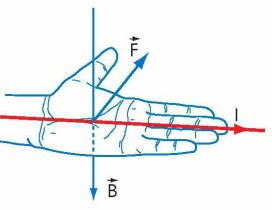
\includegraphics[width=0.3\linewidth]{figs/VN12-Y24-PH-SYL-017-8}
			\captionof{figure}{Hình vẽ mô tả quy tắc bàn tay trái.}
		\end{center}
	\end{itemize}
\end{tomtat}


\subsection{Ví dụ minh hoạ}
\begin{dang}{Vận dụng quy tắc bàn tay trái để xác định lực từ tác dụng đoạn dây dẫn mang dòng điện}
	\end{dang}
\begin{vd}
	Với mỗi trường hợp như hình, hãy xác định xem có lực từ tác dụng lên mỗi dây dẫn mang dòng điện hay không? Nếu có, hãy cho biết hướng của chúng.
	\begin{center}
		\begin{longtable}{M{8cm}M{8cm}}
			\begin{tikzpicture}
				\foreach \i in {0,1,...,4}
				\draw[blue, line width=1pt, decoration={markings, mark=at position 0.75 with {\arrow{stealth}}}, postaction={decorate}] (0, \i)--(5,\i);
				\node[right] at (5,4) {$\vec{B}$};
				\node[right, red] at (2.75,2.5) {$I$};
				\node[red] at (2.5,2.5) {\LARGE$\odot$};
			\end{tikzpicture}
			&
			\begin{tikzpicture}
				\foreach \i in {0,1,...,4}
				\draw[blue, line width=1pt, decoration={markings, mark=at position 0.75 with {\arrow{stealth}}}, postaction={decorate}] (0, \i)--(5,\i);
				\node[right] at (5,4) {$\vec{B}$};
				\node[right, red] at (2.75,1.8) {$I$};
				\draw[red, line width=1.5pt, decoration={markings, mark=at position 0.5 with {\arrow{stealth}}}, postaction={decorate}] (2.5, -0.5)--(2.5,4.5);
			\end{tikzpicture}\\
			Hình a & Hình b
		\end{longtable}
	\end{center}
	\loigiai{
		\begin{center}
			\begin{longtable}{M{8cm}M{8cm}}
				\begin{tikzpicture}
					\foreach \i in {0,1,...,4}
					\draw[blue, line width=1pt, decoration={markings, mark=at position 0.75 with {\arrow{stealth}}}, postaction={decorate}] (0, \i)--(5,\i);
					\node[right] at (5,4) {$\vec{B}$};
					\node[right, red] at (2.75,2.5) {$I$};
					\node[red] at (2.5,2.5) {\LARGE$\odot$};
					\draw[line width=1.5pt, green!75!black, -latex] (2.5,2.65)--(2.5,4.5);
					\node[right, green!75!black] at (2.5,4.5) {$\vec{F}$};
				\end{tikzpicture}
				&
				\begin{tikzpicture}
					\foreach \i in {0,1,...,4}
					\draw[blue, line width=1pt, decoration={markings, mark=at position 0.65 with {\arrow{stealth}}}, postaction={decorate}] (0, \i)--(5,\i);
					\node[right] at (5,4) {$\vec{B}$};
					\node[right, red] at (2.75,3.55) {$I$};
					\draw[red, line width=1.5pt, decoration={markings, mark=at position 0.65 with {\arrow{stealth}}}, postaction={decorate}] (2.5, -0.5)--(2.5,5.5);
					\node[green!75!black, fill=white] at(2.5,2.0) {\LARGE$\otimes$};
					\node[right, green!75!black] at (2.75,2.25) {$\vec{F}$};
				\end{tikzpicture}\\
				Hình a & Hình b
			\end{longtable}
		\end{center}
	}
\end{vd}

\begin{vd}
	Xác định chiều của dòng điện trong các hình bên dưới.
\begin{center}
		\begin{longtable}{M{8cm}M{8cm}}
		\begin{tikzpicture}
			\foreach \x in {0,1,...,3}{
				\foreach \y in {0,1,...,3}{
					\node[blue] at (\x,\y) {\LARGE$\odot$};}}
			\draw[line width=1.5pt, -latex] (1.5,1.5)--(1.5,3);
			\node[above] at (1.5,3) {$\vec{F}$};
			\node[right] at (3.1,2) {$\vec{B}$};
			\filldraw[black] (1.5,1.5) circle (2pt);
		\end{tikzpicture}
		&
		\begin{tikzpicture}
			\foreach \x in {0,1,...,3}{
				\foreach \y in {0,1,...,3}{
					\node[blue] at (\x,\y) {\LARGE$\otimes$};}}
			\draw[line width=1.5pt, -latex] (1.5,1.5)--(0,1.5);
			\node[left] at (0,1.5) {$\vec{F}$};
			\node[right] at (3.1,2) {$\vec{B}$};
			\filldraw[black] (1.5,1.5) circle (2pt);
		\end{tikzpicture}\\
		Hình a & Hình b
	\end{longtable}
\end{center}
\loigiai{
	\begin{center}
		\begin{longtable}{M{8cm}M{8cm}}
			\begin{tikzpicture}
				\foreach \x in {0,1,...,3}{
					\foreach \y in {0,1,...,3}{
						\node[blue] at (\x,\y) {\LARGE$\odot$};}}
				\draw[line width=1.5pt, -latex] (1.5,1.5)--(1.5,3);
				\draw[line width=1.5pt,red, -latex] (1.5,1.5)--(0,1.5);
				\node[above] at (1.5,3) {$\vec{F}$};
				\node[left,red] at (0,1.5) {$I$};
				\node[right] at (3.1,2) {$\vec{B}$};
				\filldraw[black] (1.5,1.5) circle (2pt);
			\end{tikzpicture}
			&
			\begin{tikzpicture}
				\foreach \x in {0,1,...,3}{
					\foreach \y in {0,1,...,3}{
						\node[blue] at (\x,\y) {\LARGE$\otimes$};}}
				\draw[line width=1.5pt, -latex] (1.5,1.5)--(0,1.5);
				\node[left] at (0,1.5) {$\vec{F}$};
				\node[right] at (3.1,2) {$\vec{B}$};
				\draw[line width=1.5pt,red, -latex] (1.5,1.5)--(1.5,3);
				\node[above,red] at (1.5,3) {$I$};
				\filldraw[black] (1.5,1.5) circle (2pt);
			\end{tikzpicture}\\
			Hình a & Hình b
		\end{longtable}
	\end{center}}
\end{vd}
\begin{dang}{Vận dụng được biểu thức tính độ lớn lực từ }
	Lực từ tác dụng lên đoạn dây dẫn chiều dài $L$ đặt trong từ trường đều $B$ có dòng điên $I$ chạy qua:
	$$F=ILB\sin\theta.$$
	\end{dang}
\begin{vd}
	Một dòng điện có cường độ $\SI{0.6}{\ampere}$ chạy dọc theo dây dẫn bằng đồng được uốn thành khung hình tam giác ABC như hình vẽ. Khung được đặt trong từ trường đều có cảm ứng từ $\SI{2.8E-4}{\tesla}$. Xác định lực từ tác dụng lên cạnh:
	\begin{center}
		\begin{tikzpicture}
			\foreach \i in {0,1,...,5}
			\draw[blue, line width=1pt, decoration={markings, mark=at position 0.15 with {\arrow{stealth}}}, postaction={decorate}] (0, -0.5+\i)--(6,-0.5+\i);
			\coordinate (A) at (1.5,0);
			\coordinate (B) at (1.5,4);
			\coordinate (C) at (4.5,4);
			\coordinate (D) at (1.7,0);
			\draw[line width=1.5pt] (A)--(B)--(C)--(D)--($(D)-(0,0.5)$);
			\draw[line width=1.5pt,-latex] ($(A)-(0,0.5)$)--($(A)+(0,1)$);
			\node[below, left] at (A) {A};
			\node[above] at (B) {B};
			\node[above] at (C) {C};
			\node[above, blue] at (1,4.5) {$\vec{B}$};
			\node[left] at (1.5,1) {$I$};
			\node[below, left] at (A) {A};
			\node[left] at ($(A)!0.5!(B)$) {$\SI{40}{\centi\meter}$};
			\node[above] at ($(B)!0.5!(C)$) {$\SI{30}{\centi\meter}$};
			\node[right] at ($(C)!0.5!(D)$) {$\SI{50}{\centi\meter}$};
		\end{tikzpicture}
	\end{center}
	\begin{enumerate}[label=\alph*)]
		\item AB.
		\item AC.
		\item BC.
	\end{enumerate}
	\loigiai{
		\begin{center}
			\begin{tikzpicture}
				\foreach \i in {0,1,...,5}
				\draw[blue, line width=1pt, decoration={markings, mark=at position 0.15 with {\arrow{stealth}}}, postaction={decorate}] (0, -0.5+\i)--(6,-0.5+\i);
				\coordinate (A) at (1.5,0);
				\coordinate (B) at (1.5,4);
				\coordinate (C) at (4.5,4);
				\coordinate (D) at (1.7,0);
				\draw[line width=1.5pt] (A)--(B)--(C)--(D)--($(D)-(0,0.5)$);
				\draw[line width=1.5pt,-latex] ($(A)-(0,0.5)$)--($(A)+(0,1)$);
				\node[below, left] at (A) {A};
				\node[above] at (B) {B};
				\node[above] at (C) {C};
				\node[above, blue] at (1,4.5) {$\vec{B}$};
				\node[below, left] at (A) {A};
				\node[circle,red,fill=white,inner sep=0pt,minimum size=0pt,] at ($(A)!0.5!(B)$) {\LARGE$\otimes$};
				\node[circle,red,fill=white,inner sep=0pt,minimum size=0pt,] at ($(C)!0.5!(D)$) {\LARGE$\odot$};
				\node[red,left] at ($(A)!0.5!(B)-(0.25,0)$) {$\vec{F}_\text{AB}$};
				\node[red,right] at ($(C)!0.5!(D)+(0.25,0)$) {$\vec{F}_\text{CA}$};
			\end{tikzpicture}
		\end{center}	
		\begin{enumerate}[label=\alph*)]
			\item Độ lớn lực từ tác dụng lên cạnh AB:
			$$F_\text{AB}=IB\cdot\text{AB}\cdot\sin\left(\overrightarrow{\text{AB}},\vec{B}\right)=\left(\SI{0.6}{\ampere}\right)\cdot\left(\SI{2.8E-4}{\tesla}\right)\cdot\left(\SI{0.4}{\meter}\right)\cdot\sin\SI{90}{\degree}=\SI{6.72E-5}{\newton}.$$
			Chiều lực từ hướng vuông góc từ ngoài vào trong trang giấy.
			\item Độ lớn lực từ tác dụng lên cạnh AC:
			$$F_\text{CA}=IB\cdot\text{CA}\cdot\sin\left(\overrightarrow{\text{CA}},\vec{B}\right)=IB\cdot\text{CA}\cdot\sin\left(\pi -\widehat{BCA}\right)$$
			$$\Rightarrow F_\text{CA}=I\cdot B\cdot\text{CA}\cdot\sin\widehat{BCA}=IB\cdot\text{CA}\cdot\dfrac{\text{AB}}{\text{CA}}=\left(\SI{0.6}{\ampere}\right)\cdot\left(\SI{2.8E-4}{\tesla}\right)\cdot\left(\SI{0.5}{\meter}\right)\cdot\left(\dfrac{\SI{40}{\centi\meter}}{\SI{50}{\centi\meter}}\right)=\SI{6.72E-5}{\newton}.$$
			Chiều lực từ hướng vuông góc từ trong ra ngoài trang giấy.
			\item $F_\text{BC}=0$ vì $\left(\overrightarrow{\text{BC}},\vec{B}\right)=\SI{0}{\degree}$.
		\end{enumerate}
	}
\end{vd}

\begin{vd}
	Một dây dẫn thẳng MN chiều dài $\ell$, khối lượng của một đơn vị dài của dây là $d=\SI{0.04}{\kilogram/\meter}$. Dây dẫn được treo bằng hai dây dẫn nhẹ thẳng đứng và đặt trong từ trường đều có $\vec{B}$ vuông góc với mặt phẳng chứa MN và dây treo như hình bên dưới, độ lớn $B=\SI{0.04}{\tesla}$. Cho dòng điện có cường độ $I$ đi qua dây dẫn.
	\begin{center}
		\begin{tikzpicture}
			\coordinate (A) at (0,0);
			\coordinate (B) at (4,0);
			\coordinate (C) at (2,-4);
			\draw[line width=1pt] (A)--($(A)-(0,4)$);
			\draw[line width=1pt] (B)--($(B)-(0,4)$);
			\node[draw, line width=1pt, fill=black, shape=rectangle, minimum width=0.8cm, minimum height=0.3cm, anchor=center] at (A) {};
			\node[draw, line width=1pt, fill=black, shape=rectangle, minimum width=0.8cm, minimum height=0.3cm, anchor=center] at (B) {};
			\node[draw, line width=1pt, fill=orange!90!black, shape=rectangle, minimum width=5cm, minimum height=0.4cm, anchor=center] at (C) {};
			\node[below] at ($(A)+(-0.5,-4.25)$) {M};
			\node[below] at ($(B)+(0.5,-4.25)$) {N};
			\node[below] at ($(A)!0.5!(B)-(0,4.25)$) {$\ell$};
			\node[red] at ($(A)!0.5!(B)-(0,2)$) {\LARGE$\otimes$};
			\node[red, right] at ($(A)!0.5!(B)-(-0.25,2)$) {$\vec{B}$};
			
			
		\end{tikzpicture}
	\end{center}
	\begin{enumerate}[label=\alph*)]
		\item Xác định chiều và độ lớn của $I$ để lực căng của các dây treo bằng 0.
		\item Cho $\text{MN}=\SI{25}{\centi\meter}$, dòng điện qua dây dẫn có cường độ $I'=\SI{16}{\ampere}$ và có chiều từ N đến M. Tính lực căng mỗi dây trong trường hợp này. Lấy $g=\SI{10}{\meter/\second^2}$.
	\end{enumerate}
	\loigiai{Khối lượng dây $m=d\cdot\ell$.
		\begin{enumerate}[label=\alph*)]
			\item Để lực căng của các dây treo bằng 0 thì lực từ $\vec{F}$ phải cùng phương, ngược chiều và bằng về độ lớn với trọng lượng $\vec{P}$ như hình vẽ.\\\
			\begin{minipage}{0.6\textwidth}
				Áp dụng quy tắc bàn tay trái, để lực từ $\vec{F}$ cùng phương, ngược chiều $\vec{P}$ thì chiều dòng điện phải đi từ M đến N.\\
				Từ $F=P\Leftrightarrow I\ell B=mg$
				$$\Leftrightarrow I=\dfrac{mg}{B\ell}=\dfrac{gd}{B}=\dfrac{\left(\SI{0.04}{\kilogram/\meter}\right)\cdot\left(\SI{10}{\meter/\second^2}\right)}{\SI{0.04}{\tesla}}=\SI{10}{\ampere}.$$
			\end{minipage}
			\hfill
			\begin{minipage}{0.4\textwidth}
				\centering
				\begin{tikzpicture}
					\coordinate (A) at (0,0);
					\coordinate (B) at (3,0);
					\coordinate (C) at ($(A)!0.5!(B)-(0,3)$);
					\draw[line width=1pt] (A)--($(A)-(0,3)$);
					\draw[line width=1pt] (B)--($(B)-(0,3)$);
					\node[draw, line width=1pt, fill=black, shape=rectangle, minimum width=0.8cm, minimum height=0.3cm, anchor=center] at (A) {};
					\node[draw, line width=1pt, fill=black, shape=rectangle, minimum width=0.8cm, minimum height=0.3cm, anchor=center] at (B) {};
					\node[draw, line width=1pt, fill=orange!90!black, shape=rectangle, minimum width=4cm, minimum height=0.4cm, anchor=center] at (C) {};
					\node[below] at ($(A)+(-0.5,-3.25)$) {M};
					\node[below] at ($(B)+(0.5,-3.25)$) {N};
					\node[red] at ($(A)!0.5!(B)-(0,0.5)$) {\LARGE$\otimes$};
					\node[red, right] at ($(A)!0.5!(B)-(-0.25,0.5)$) {$\vec{B}$};
					
					\filldraw[black] (C) circle (2pt);
					\draw[-stealth, green!75!black, line width=1.5pt] (C)--($(C)+(0,1.5)$);
					\draw[-stealth, green!75!black,line width=1.5pt] (C)--($(C)-(0,1.5)$);
					\node[right, green!75!black] at ($(C)+(0,1.5)$) {$\vec{F}$};
					\node[right, green!75!black] at ($(C)+(0,-1.5)$) {$\vec{P}$};
				\end{tikzpicture}
			\end{minipage}
			\item Khi $I'=\SI{16}{\ampere}$, ta có:\\
			\begin{minipage}{0.6\textwidth}
				\begin{itemize}
					\item Lực từ $\vec{F}$ tác dụng lên thanh có độ lớn:
					$$F'=I'\ell B=\SI{0.16}{\newton}.$$
					\item Khối lượng dây:
					$$m=\ell d=\SI{0.01}{\kilogram}.$$
					\item Trọng lượng của thanh:
					$$P=mg=\SI{0.1}{\newton}.$$
				\end{itemize}
				Do $I'$ có chiều từ N đến M nên $\vec{F}'$ cùng phương, cùng chiều với $\vec{P}$.\\
				$\Rightarrow$ Lực căng mỗi dây: $T=\dfrac{P+F'}{2}=\SI{0.13}{\newton}.$
			\end{minipage}
			\hfill
			\begin{minipage}{0.4\textwidth}
				\centering
				\begin{tikzpicture}
					\coordinate (A) at (0,0);
					\coordinate (B) at (3,0);
					\coordinate (C) at ($(A)!0.5!(B)-(0,3)$);
					\draw[line width=1pt] (A)--($(A)-(0,3)$);
					\draw[line width=1pt] (B)--($(B)-(0,3)$);
					\draw[purple, line width=1.5pt,-stealth] ($(A)-(0,3)$)--($(A)-(0,1.5)$);
					\draw[purple, line width=1.5pt,-stealth] ($(B)-(0,3)$)--($(B)-(0,1.5)$);
					\node[draw, line width=1pt, fill=black, shape=rectangle, minimum width=0.8cm, minimum height=0.3cm, anchor=center] at (A) {};
					\node[draw, line width=1pt, fill=black, shape=rectangle, minimum width=0.8cm, minimum height=0.3cm, anchor=center] at (B) {};
					\node[draw, line width=1pt, fill=orange!90!black, shape=rectangle, minimum width=4cm, minimum height=0.4cm, anchor=center] at (C) {};
					\node[below] at ($(A)+(-0.5,-3.25)$) {M};
					\node[below] at ($(B)+(0.5,-3.25)$) {N};
					\node[red] at ($(A)!0.5!(B)-(0,0.5)$) {\LARGE$\otimes$};
					\node[red, right] at ($(A)!0.5!(B)-(-0.25,0.5)$) {$\vec{B}$};
					
					\filldraw[black] (C) circle (2pt);
					\draw[-stealth, blue, line width=1.5pt] (C)--($(C)+(0,-2)$);
					\draw[-stealth, green!75!black,line width=1.5pt] (C)--($(C)-(0,1.5)$);
					\node[right, blue] at ($(C)+(0,-2)$) {$\vec{F}'$};
					\node[right, green!75!black] at ($(C)+(0,-1.5)$) {$\vec{P}$};
					\node[right, purple] at ($(B)-(0,1.5)$) {$\vec{T}$};
					\node[left, purple] at ($(A)-(0,1.5)$) {$\vec{T}$};
				\end{tikzpicture}
			\end{minipage}
		\end{enumerate}
		
	}
\end{vd}
\begin{vd}
	Treo đoạn dây dẫn $\text{MN}=\SI{5}{\centi\meter}$ khối lượng $\SI{5}{\gram}$ bằng hai dây không dãn, khối lượng không đáng kể. Không gian có từ trường đều với vector cảm ứng từ có phương vuông góc với đoạn dây, chiều từ trên xuống và có độ lớn $B=\SI{0.5}{\tesla}$. Tính góc lệch của dây treo so với phương thẳng đứng khi đoạn dây MN nằm cân bằng, biết cường độ dòng điện qua đoạn dây MN là $\SI{2}{\ampere}$, lấy $g=\SI{10}{\meter/\second^2}$.
	\begin{center}
		\begin{tikzpicture}
			\coordinate (A) at (0,0);
			\coordinate (B) at (4,0);
			\coordinate (C) at (2,-4);
			\draw[line width=1pt] (A)--($(A)-(0,4)$);
			\draw[line width=1pt] (B)--($(B)-(0,4)$);
			\node[draw, line width=1pt, fill=black, shape=rectangle, minimum width=0.8cm, minimum height=0.3cm, anchor=center] at (A) {};
			\node[draw, line width=1pt, fill=black, shape=rectangle, minimum width=0.8cm, minimum height=0.3cm, anchor=center] at (B) {};
			\node[draw, line width=1pt, fill=orange!90!black, shape=rectangle, minimum width=5cm, minimum height=0.4cm, anchor=center] at (C) {};
			\node[below] at ($(A)+(-0.5,-4.25)$) {M};
			\node[below] at ($(B)+(0.5,-4.25)$) {N};
			\node[below] at ($(A)!0.5!(B)-(0,4.25)$) {$\ell$};
			\node[red, right] at ($(A)!0.5!(B)-(0,2.5)$) {$\vec{B}$};
			\draw[-stealth, red, line width=1.5pt] ($(A)!0.5!(B)-(0,1)$)--($(A)!0.5!(B)-(0,2.5)$);
			
		\end{tikzpicture}
	\end{center}
	\loigiai{
		\begin{center}
			\begin{tikzpicture}
				\coordinate (O) at(0,0);
				\coordinate (A) at (-45:4);
				\coordinate (B) at (-90:4);
				\node[draw, line width=1pt, fill=black, shape=rectangle, minimum width=1cm, minimum height=0.3cm, anchor=center] at (O) {};
				\draw[line width=1.5pt] (O)--(A);
				\draw[line width=1.5pt, dashed] (O)--(B);
				\draw[line width=1.5pt, -stealth, blue] (A)--($(A)-(0,1.5)$);
				\draw[line width=1.5pt, -stealth, red] (A)--($(A)+(1.5,0)$);
				\draw[line width=1.5pt, -stealth, green!60!black] (A)--($(A)+(135:1.5)$);
				\draw[-stealth, red, line width=1.5pt] (-0.5,-0.5)--(-0.5,-2.5);
				\node[red,left] at (-0.5,-2.5) {$\vec{B}$};
				\node[circle,red,fill=white,inner sep=0pt,minimum size=0pt,] at (A) {\LARGE$\odot$};
				\node[green!60!black, above right] at ($(A)+(135:1.5)$) {$\vec{T}$};
				\node[blue, right] at ($(A)-(0,1.5)$) {$\vec{P}$};
				\node[red, above] at ($(A)+(1.5,0)$) {$\vec{F}$};
				\tkzMarkAngle[color=black, line width=1.25pt](B,O,A);
				\tkzLabelAngle[color=black,pos=1.2](B,O,A){$\alpha$}
			\end{tikzpicture}
		\end{center}
		Dây dẫn nằm cân bằng nên:
		$$\vec{P}+\vec{F}+\vec{T}=\vec{0}$$
		Từ đó, ta có:
		$$\tan\alpha=\dfrac{F}{P}=\dfrac{I\ell B\sin\SI{90}{\degree}}{mg}=1\Rightarrow \alpha=\SI{45}{\degree}.$$
	}
\end{vd}
\subsection{Bài tập}
\subsubsection{Trắc nghiệm nhiều phương án lựa chọn}
\setcounter{ex}{0}
\Opensolutionfile{ans}[ans/VN12-Y24-PH-SYL-018P-TN]
% ===================================================================
\begin{ex}
	Cho các phát biểu sau đây:
	\begin{enumerate}[label=(\arabic*)]
		\item Từ trường có thể tác dụng lực từ lên các điện tích đứng yên đặt trong nó.
		\item Từ trường có khả năng tác dụng lực từ lên dòng điện đặt trong nó.
		\item Từ trường có khả năng tác dụng lực từ lên nam châm đặt trong nó.
		\item Đường sức từ luôn là những đường cong khép kín.
	\end{enumerate}	
	Trong các phát biểu trên, số phát biểu đúng là
	\choice
	{1}
	{2}
	{\True 3}
	{4}
	\loigiai{Các phát biểu đúng là (2), (3), (4)}
\end{ex}

% ===================================================================
\begin{ex}
	Trong hệ SI, đơn vị đo độ lớn cảm ứng từ là 	
	\choice
	{fara $\left(\si{\farad}\right)$}
	{henry $\left(\si{\ohm}\right)$}
	{\True tesla $\left(\si{\tesla}\right)$}
	{ampere $\left(\si{\ampere}\right)$}
	\loigiai{}
\end{ex}
% ===================================================================
\begin{ex}
	Đặt một dây dẫn có chiều dài là $\ell$, mang dòng điện $I$ trong từ trường đều có độ lớn cảm ứng từ $B$ và tạo với cảm ứng từ góc $\theta$. Lực do từ trường tác dụng lên dây dẫn có độ lớn là
	\choice
	{$\dfrac{I\ell}{B}\sin\theta$}
	{$BI\ell \cos\theta$}
	{\True $BI\ell\sin\theta$}
	{$I^2\ell B\sin\theta$}
	\loigiai{}
\end{ex}



% ===================================================================
\begin{ex}
	Chọn cụm từ và công thức phù hợp để điền vào chỗ trống.\\
	Cảm ứng từ là một đại lượng (1)\dots, đặc trưng cho từ trường về phương diện tác dụng lực. Khi một đoạn dây dẫn thẳng có chiều dài $L$, mang dòng điện có cường độ $I$ được đặt trong vùng từ trường đều có cảm ứng từ $\vec{B}$ hợp với chiều dòng điện một góc $\theta$ thì độ lớn cảm ứng từ được xác định bởi biểu thức (2) \dots
	\choice
	{(1) vô hướng, (2) $B=\dfrac{F}{IL\cos\theta}$}
	{\True (1) vector, (2) $B=\dfrac{F}{IL\sin\theta}$}
	{(1) vô hướng, (2) $B=\dfrac{F}{IL\sin\theta}$}
	{(1) vector, (2) $B=\dfrac{F}{IL\cos\theta}$}
	\loigiai{}
\end{ex}
% ===================================================================
\begin{ex}
	Tìm phát biểu \textbf{đúng} trong các phát biểu sau.\\
	Một dòng điện đặt vuông góc với đường sức từ trong từ trường, chiều của lực từ tác dụng vào dòng điện sẽ không thay đổi khi
	\choice
	{đổi chiều dòng điện ngược lại}
	{đổi chiều cảm ứng từ ngược lại}
	{\True đồng thời đổi chiều dòng điện và đổi chiều cảm ứng từ}
	{quay dòng điện một góc $90^{\circ}$ xung quanh đường sức từ}
	\loigiai{}
\end{ex}
% ===================================================================
\begin{ex}
	Chỉ ra phát biểu \textbf{sai}.
	\choice
	{Lực từ tác dụng lên đoạn dây dẫn mang dòng điện có phương vuông góc với dòng điện}
	{Lực từ tác dụng lên đoạn dây dẫn mang dòng điện có phương vuông góc với đường cảm ứng từ}
	{\True Lực từ tác dụng lên đoạn dây dẫn mang dòng điện có phương vuông góc với mặt phẳng chứa dòng điện và đường cảm ứng từ}
	{Lực từ tác dụng lên đoạn dây dẫn mang dòng điện có phương tiếp tuyến với các đường cảm ứng từ}
	\loigiai{}
\end{ex}
% ===================================================================
\begin{ex}
	Phát biểu nào sau đây \textbf{không đúng}?	
	\choice
	{Lực từ tác dụng lên một đoạn dây dẫn mang dòng điện đặt trong từ trường đều tỉ lệ thuận với cường độ dòng điện chạy qua đoạn dây dẫn}
	{Lực từ tác dụng lên một đoạn dây dẫn mang dòng điện đặt trong từ trường đều tỉ lệ thuận với chiều dài của đoạn dây dẫn}
	{Lực từ tác dụng lên một đoạn dây dẫn mang dòng điện đặt trong từ trường đều tỉ lệ thuận với cảm ứng từ tại điểm đặt đoạn dây dẫn}
	{\True Lực từ tác dụng lên một đoạn dây dẫn mang dòng điện đặt trong từ trường đều tỉ lệ thuận với góc hợp bởi đoạn dây dẫn và đường sức từ}
	\loigiai{$$F=ILB\sin\theta.$$}
\end{ex}
% ===================================================================
\begin{ex}
	Phát biểu nào dưới đây \textbf{đúng}?\\
	Cho một đoạn dây dẫn mang dòng điện $I$ đặt song song với đường sức từ, chiều của dòng điện ngược chiều với chiều của đường sức từ.
	\choice
	{\True Lực từ luôn bằng không khi tăng cường độ dòng điện}
	{Lực từ tăng khi tăng cường độ dòng điện}
	{Lực từ giảm khi tăng cường độ dòng điện}
	{Lực từ đổi chiều khi ta đổi chiều dòng điện}
	\loigiai{}
\end{ex}
% ===================================================================
\begin{ex}
	Một dây dẫn được đặt nằm ngang theo hướng nam bắc trong một từ trường đều có cảm ứng từ nằm ngang hướng về phía đông. Trong dây dẫn có dòng electron chuyển động theo chiều về phía nam. Phát biểu nào sau đây là \textbf{đúng}?
	\choice
	{Lực tác dụng lên dây có hướng là hướng đông}
	{\True Lực tác dụng lên dây có hướng vuông góc và đi vào trang giấy}
	{Lực tác dụng lên dây có hướng vuông góc và ra khỏi trang giấy}
	{Không có lực từ tác dụng lên dây}
	\loigiai{}
\end{ex}
% ===================================================================
\begin{ex}
	Khi sét đánh, có dòng điện tích âm chuyển động từ đám mây xuống mặt đất. Từ trường của Trái Đất hướng về phía bắc. Tia sét bị từ trường Trái Đất làm chệch hướng theo hướng nào?
	
	\choice
	{Bắc}
	{Nam}
	{Đông}
	{\True Tây}
	\loigiai{Áp dụng quy tắc bàn tay trái, từ trường hướng về phía Bắc, dòng điện gây ra bởi tia sét hướng lên trên $\Rightarrow$ lực từ tác dụng lên tia sét hướng về phía Tây.}
\end{ex}

% ===================================================================
\begin{ex}
	Hai dây dẫn thẳng, dài, đặt vuông góc với nhau, rất gần nhau nhưng không chạm vào nhau. Dòng điện qua hai dây dẫn có chiều như hình vẽ và có cùng cường độ. Từ trường do hai dây dẫn gây ra có thể triệt tiêu nhau trong vùng nào?
	\begin{center}
		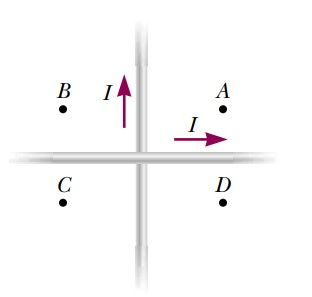
\includegraphics[width=0.3\linewidth]{figs/VN12-Y24-PH-SYL-017P-8}
	\end{center}
	\choice
	{vùng A và D}
	{\True vùng A và C}
	{vùng B và D}
	{vùng B và C}
	\loigiai{}
\end{ex}
% ===================================================================
\begin{ex}
	Xét dây dẫn có chiều dài $L$, có dòng điện $I$ chạy qua đặt tại điểm M trong từ trường đều, chịu tác dụng của lực điện từ $F$. Khi thay đổi $L$ hoặc $I$ thì $F$ thay đổi nhưng tỉ số nào sau đây luôn không đổi?
	\choice
	{$\frac{FI}{2L}$}
	{\True $\frac{F}{IL}$}
	{$\frac{FL}{I}$}
	{$\frac{FI^2}{L}$}
	\loigiai{}
\end{ex}
% ===================================================================
\begin{ex}
	Một đoạn dây dẫn đặt trong từ trường đều. Nếu chiều dài dây dẫn và cường độ dòng điện qua dây dẫn tăng 2 lần thì độ lớn lực từ tác dụng lên dây dẫn	
	\choice
	{tăng 2 lần}
	{giảm 2 lần}
	{\True tăng 4 lần}
	{không đổi}
	\loigiai{
		$$F=ILB\sin\theta.$$
	}
\end{ex}

% ===================================================================
\begin{ex}
	Một đoạn dây dẫn mang dòng điện được đặt vuông góc với từ trường đều có cảm ứng từ $B$. Khi dòng điện trong dây là $I$ thì lực từ tác dụng lên đoạn dây đó là $F$. Cũng đoạn dây đó, cho dòng điện chạy qua dây là $0,25I$ và đặt trong từ trường $2B$, lực từ tác dụng lên đoạn dây đó là
	\choice
	{$\dfrac{F}{4}$}
	{\True $\dfrac{F}{2}$}
	{$F$}
	{$2F$}
	\loigiai{}
\end{ex}
% ===================================================================
\begin{ex}
	Trong thí nghiệm đo độ lớn cảm ứng từ bằng "cân dòng điện" với bố trí thí nghiệm được thể hiện như trong hình \ref{fig:18P-11}, khung dây được sử dụng có kích thước là $\SI{100}{\milli\meter}\times\SI{80}{\milli\meter}$ như hình \ref{fig:18P-12}. Nếu ta thay khung dây ban đầu thành một khung dây khác có kích thước là $\SI{100}{\milli\meter}\times\SI{20}{\milli\meter}$ nhưng vẫn giữ nguyên góc hợp bởi mặt phẳng khung dây và các đường sức từ cũng như cường độ dòng điện qua khung dây và nam châm điện thì nhận định nào sau đây về lực từ do từ trường tác dụng lên khung dây là \textbf{đúng}?
	\begin{center}
		\begin{tabular}{M{8cm}M{8cm}}
			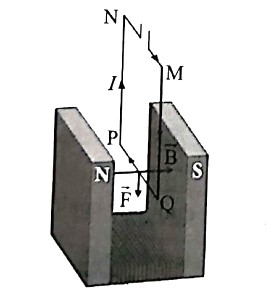
\includegraphics[width=0.6\linewidth]{figs/VN12-Y24-PH-SYL-018P-11}
			\captionof{figure}{}
			\label{fig:18P-11}
			&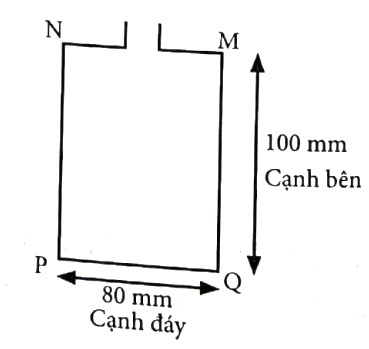
\includegraphics[width=0.6\linewidth]{figs/VN12-Y24-PH-SYL-018P-12}
			\captionof{figure}{}
			\label{fig:18P-12}
		\end{tabular}
	\end{center}
	\choice
	{Không đổi chiều và độ lớn tăng 4 lần}
	{\True Không đổi chiều và độ lớn giảm 4 lần}
	{Đổi chiều và độ lớn giảm 4 lần}
	{Đổi chiều và độ lớn tăng 4 lần}
	\loigiai{
		Vi từ trường chỉ tác dụng lực lên cạnh dưới của khung và độ lớn của lực từ được xác định bằng biểu thức $F=B I L$ nên khi chiều dài cạnh đáy giảm 4 lần thì độ lớn lực từ giảm 4 lần.
	}
\end{ex}


% ===================================================================
\begin{ex}
	Một đoạn dây dẫn dài $\ell=\SI{0.8}{\meter}$ đặt trong từ trường đều sao cho dây dẫn hợp với vector cảm ứng từ một góc $\SI{60}{\degree}$. Biết dòng điện $I=\SI{20}{\ampere}$ và dây dẫn chịu một lực là $F=\SI{2E-2}{\newton}$. Độ lớn của cảm ứng từ là
	\choice
	{$\SI{0.8E-3}{\tesla}$}
	{$\SI{E-3}{\tesla}$}
	{\True $\SI{1.4E-3}{\tesla}$}
	{$\SI{1.6E-3}{\tesla}$}
	\loigiai{
		$$B=\dfrac{F}{I\ell\sin\theta}=\dfrac{\SI{2E-2}{\newton}}{\left(\SI{20}{\ampere}\right)\cdot\left(\SI{0.8}{\meter}\right)\cdot\sin\SI{60}{\degree}}\approx\SI{1.44E-3}{\tesla}.$$
	}
\end{ex}

% ===================================================================
\begin{ex}
	Một đoạn dây dẫn dài $\SI{2}{\centi\meter}$ nằm trong từ trường, dòng điện chạy qua có cường độ $\SI{1}{\ampere}$. Một nam châm tạo từ trường có cường độ cảm ứng từ $\SI{0.5}{\tesla}$ và hợp với dây dẫn một góc $\SI{30}{\degree}$. Lực từ tác dụng lên dây dẫn có độ lớn là
	
	\choice
	{$\SI{10E-2}{\newton}$}
	{$\SI{1E-2}{\newton}$}
	{\True $\SI{0.5E-2}{\newton}$}
	{$\SI{50E-2}{\newton}$}
	\loigiai{
		$$
		F=BIL\sin \alpha=\SI{0.5E-2}{\newton}.
		$$
		
	}
\end{ex}
% ===================================================================
\begin{ex}
	Khi góc hợp bởi vector cảm ứng từ với đoạn dây dẫn có dòng điện là $\alpha=\SI{90}{\degree}$ thì lực từ tác dụng có giá trị là $\SI{0.4}{\newton}$. Nếu thay đổi góc $\alpha$ nhỏ dần đến $\SI{0}{\degree}$, thì lực tác dụng thay đổi như thế nào?
	\choice
	{\True Lực cũng giảm dần đến 0}
	{Lực tăng lên đến $\SI{0.8}{\newton}$}
	{Lực không đổi}
	{Lực giảm xuống $\SI{0.2}{\newton}$}
	\loigiai{}
\end{ex}

% ===================================================================
\begin{ex}
	Một dây dẫn thẳng có chiều dài $\SI{3.0}{\meter}$ mang dòng điện $\SI{6.0}{\ampere}$ được đặt nằm ngang, hướng của dòng điện tạo với hướng bắc một góc $\SI{50}{\degree}$ lệch về phía tây. Tại điểm này, cảm ứng từ của từ trường Trái Đất có độ lớn là $\SI{0.14E-4}{\tesla}$ và hướng bắc. Lực tác dụng lên dây có độ lớn là
	\choice
	{$\SI{0.28E-4}{\newton}$}
	{$\SI{2.5E-4}{\newton}$}
	{$\SI{1.9E-4}{\newton}$}
	{\True $\SI{1.6E-4}{\newton}$}
	\loigiai{
		$$F=ILB\sin\SI{50}{\degree}\approx\SI{1.6E-4}{\newton}.$$	
	}
\end{ex}
% ===================================================================
\begin{ex}
	Một dây đồng dài $\SI{25}{\centi\meter}$, có khối lượng là $\SI{10}{\gram}$ nằm trong từ trường $\SI{0.20}{\tesla}$. Lấy gia tốc trọng trường $g=\SI{10}{\meter/\second^2}$. Cường độ dòng điện nhỏ nhất chạy qua dây gây ra lực từ có độ lớn bằng trọng lượng của dây là
	\choice
	{$\SI{1.3}{\ampere}$}
	{$\SI{1.5}{\ampere}$}
	{\True $\SI{2.0}{\ampere}$}
	{$\SI{4.9}{\ampere}$}
	\loigiai{
		$$I_\text{min}=\dfrac{P}{BL\left(\sin\theta\right)_{\text{max}}}=\SI{2.0}{\ampere}.$$	
	}
\end{ex}
% ===================================================================
\begin{ex}
	Trong thí nghiệm xác định độ lớn cảm ứng từ của nam châm điện chữ $U$ bằng "cân dòng điện" (theo phương án thí nghiệm trong Bài 11 của SGK CTST), xét trạng thái ổn định với đòn cân nằm ngang cân bằng khi có dòng điện chạy trong khung dây và nam châm điện, góc hợp bởi mặt phẳng khung dây và các đường sức từ là $\SI{90}{\degree}$. Nếu ta làm khung dây bị lệch một góc nào đó so với vị trí ban đầu thì khi đòn cân được điều chỉnh trở về lại trạng thái nằm ngang cân bằng, số chỉ của lực kế sẽ	
	\choice
	{vẫn giữ nguyên giá trị ban đầu}
	{lớn hơn giá trị ban đầu}
	{\True nhỏ hơn giá trị ban đầu}
	{dao động xung quanh giá trị ban đầu}
	\loigiai{
		Vì độ lớn của lực từ được xác định bằng biểu thức $F=ILB\sin\theta$ nên khi khung dây bị lệch so với ban đầu thì $\sin\theta$ giảm dẫn đến $F$ giảm. Vì vậy số chỉ của lực kế giảm so với ban đầu.	
	}
\end{ex}


% ===================================================================
\begin{ex}
	Thanh dây dẫn thẳng MN có chiều dài $\SI{20}{\centi\meter}$, khối lượng $\SI{10}{\gram}$, được treo trên hai sợi dây mảnh sao cho MN nằm ngang. Cả hệ thống được đặt trong từ trường đều có cảm ứng từ $B=\SI{0.25}{\tesla}$ và vector $\vec{B}$ hướng lên trên theo phương thẳng đứng. Nếu cho dòng điện $I=\xsi{2\sqrt{3}}{\ampere}$ chạy qua, người ta thấy thanh MN được nâng lên vị trí cân bằng mới và hai sợi dây treo bây giờ lệch một góc $\alpha$ so với phương thẳng đứng. Cho $g=\SI{10}{\meter/\second^2}$, góc lệch $\alpha$ là	
	\begin{center}
		\begin{tikzpicture}
			\coordinate (A) at (0,0);
			\coordinate (B) at (3,1.5);
			\coordinate (A1) at ($(A)+(0,-1.5)$);
			\coordinate (B1) at ($(B)+(0,-1.5)$);
			\coordinate (M) at ($(A)+(-30:3)$);
			\coordinate (N) at ($(B)+(-30:3)$);
			\draw[line width=1pt] (A)--(M);
			\draw[line width=1pt] (B)--(N);
			\draw[line width=1pt, dashed] (A)--(A1);
			\draw[line width=1pt, dashed] (B)--(B1);
			\draw[line width=4pt] (M)--(N);
			\draw[line width=3pt, blue] (A)--+(30:0.5)--+(-150:0.5);
			\draw[line width=3pt, blue] (B)--+(30:0.5)--+(-150:0.5);
			\tkzMarkAngle[size=0.75cm,color=red](A1,A,M);
			\tkzLabelAngle[color=red,pos=1.2](A1,A,M){$\alpha$};
		\end{tikzpicture}
	\end{center}
	\choice
	{$\SI{30}{\degree}$}
	{$\SI{45}{\degree}$}
	{\True $\SI{60}{\degree}$}
	{$\SI{90}{\degree}$}
	\loigiai{}
\end{ex}

\Closesolutionfile{ans}

\subsubsection{Trắc nghiệm đúng/sai}
\Opensolutionfile{ans}[ans/VN12-Y24-PH-SYL-018P-TF]
\setcounter{ex}{0}
% ===================================================================
\begin{ex}
	Một thí nghiệm để tìm ra lực từ tác dụng lên một đoạn dây dẫn chứa dòng điện được đặt trong từ trường của một nam châm.
	\choiceTF[t]
	{\True Nếu cường độ dòng điện qua dây tăng lên, lực từ tác dụng lên dây sẽ tăng lên}
	{Nếu khoảng cách giữa dây dẫn và nam châm tăng lên, lực từ tác dụng lên dây sẽ tăng lên}
	{\True Lực từ chỉ có thể tác dụng lên dây dẫn khi có dòng điện chạy qua dây}
	{Độ lớn lực từ tác dụng lên đoạn dây dẫn sẽ thay đổi khi dòng điện chạy qua dây đảo chiều}
	\loigiai{}
\end{ex}
% ===================================================================
\begin{ex}
	Trong mỗi phát biểu sau, em hãy chọn đúng hoặc sai.	
	\choiceTF[t]
	{Cảm ứng từ là một đại lượng vô hướng}
	{\True Tiếp tuyến tại bất kì điểm nào trên đường sức từ đều có phương, chiều trùng với phương, chiều của vector cảm ứng từ tại điểm đó}
	{\True Từ trường ở vùng không gian giữa hai cực của nam châm chữ U được xem là từ trường đều}
	{Trong từ trường đều, các đường sức từ song song nhau nhưng vector cảm ứng từ tại các điểm khác nhau lại không bằng nhau về độ lớn}
	\loigiai{}
\end{ex}
% ===================================================================
\begin{ex}
	\immini{Xét một dây dẫn thẳng dài vô hạn có dòng điện cường độ $I$ chạy qua. Hai điểm M, N nằm trong cùng một mặt phẳng vuông góc với dây dẫn và cách đều dây dẫn, biết OM vuông góc với ON.\\
		Trong mỗi phát biểu sau về cảm ứng từ tại điểm M và N do dòng điện này gây ra, em hãy chọn đúng hoặc sai.	}
	{		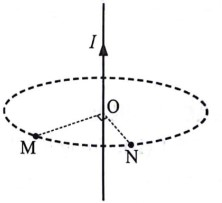
\includegraphics[width=0.4\linewidth]{figs/VN12-Y24-PH-SYL-018P-1}
	}
	
	\choiceTF[t]
	{\True Cảm ứng từ tại điểm M có phương vuông góc với OM}
	{cảm ứng từ tại điểm N song song với dây dẫn và có hướng cùng chiều với dòng điện chạy trong dây dẫn}
	{\True M và N cùng nằm trên một đường sức từ}
	{\True Cảm ứng từ tại M và N bằng nhau về độ lớn}
	\loigiai{}
\end{ex}

% ===================================================================
\begin{ex}
	Chỉ ra đáp án đúng, đáp án sai.
	\choiceTF[t]
	{\True Nam châm tác dụng lên dòng điện thực chất là tương tác giữa từ trường của nam châm với các electron của dây điện}
	{Nam châm tác dụng lên dòng điện thực chất là tương tác giữa từ trường của nam châm với từ trường do các electron chuyển động gây ra}
	{Phương của lực từ trùng với phương của dòng điện}
	{\True Lực từ tác dụng lên đoạn dây dẫn mang dòng điện có phương vuông góc với đoạn dây dẫn và vuông góc vector cảm ứng từ}
	\loigiai{}
\end{ex}
% ===================================================================
\begin{ex}
	Trong mỗi nhận định sau về thí nghiệm đo độ lớn cảm ứng từ bằng "cân dòng điện" với bố trí thí nghiệm được thể hiện như hình \ref{fig:18P-10}. Em hãy chọn đúng hoặc sai cho mỗi nhận định sau đây.
	\begin{center}
		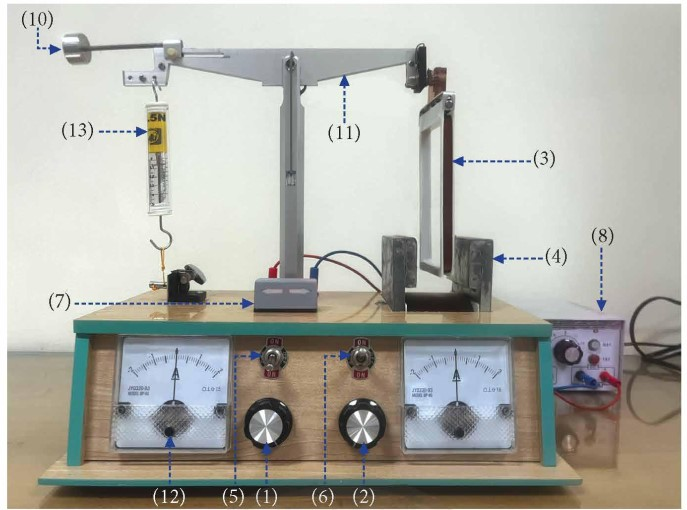
\includegraphics[width=0.55\linewidth]{figs/VN12-Y24-PH-SYL-018P-10}
		\captionof{figure}{Thí nghiệm đo độ lớn cảm ứng từ bằng "cân dòng điện"}
		\label{fig:18P-10}
	\end{center}
	\choiceTFt
	{\True Cơ sở lí thuyết của thí nghiệm này dựa trên tác dụng lực của từ trường đều lên đoạn dây dẫn có dòng điện chạy qua}
	{\True Trước khi bật công tắc cho dòng điện chạy qua khung dây dẫn và nam châm điện, cần phải điều chỉnh sao cho đòn cân nằm ngang rồi đọc giá trị của lực kế}
	{Khi đóng công tắc cho dòng điện chạy qua khung dây dẫn và nam châm điện, từ trường tạo ra bởi nam châm luôn tác dụng lực đẩy khung dây đi lên}
	{\True Trong thí nghiệm, từ trường tạo bởi nam châm điện không tác dụng lực từ lên các cạnh bên của khung dây}
	{Từ trường trong vùng không gian giữa hai nhánh của nam châm điện trong thí nghiệm được xem gần đúng là từ trường đều. Chiều và độ lớn của vector cảm ứng từ trong vùng từ trường này không phụ thuộc vào chiều và cường độ dòng điện chạy qua cuộn dây của nam châm}
	{Có thể lấy giá trị của lực kế khi đòn cân chưa nằm ngang ổn định}
	{\True Công dụng của các núm xoay (1) và (2) là điều chỉnh giá trị cường độ dòng điện chạy qua khung dây và cuộn dây của nam châm điện}
	{\True Có thể thay đổi chiều của lực từ tác dụng lên khung dây bằng việc sử dụng công tắc (5) hoặc (6)}
	\loigiai{}
\end{ex}

% ===================================================================
\begin{ex}
	Cho một khung dây dẫn hình chữ nhật có chiều rộng $\SI{20}{\centi\meter}$, mang dòng điện, đặt trong từ trường đều có cảm ứng từ $\vec{B}$ hướng vào trong như hình vẽ. Biết mặt phẳng vòng dây vuông góc với các đường sức từ. Bên ngoài vòng tròn, từ trường bằng 0.\begin{center}
		\begin{tikzpicture}
			\foreach \x in {-3,-2,...,3}{
				\foreach \y in {-3,-2,...,3}{
					\node[blue] at (\x,\y) {\LARGE$\odot$};
					
			}}
			\fill[white, even odd rule] (0,0) circle(3.4) (0,0) circle (4.5);
			\draw[dashed, line width=1pt] (0,0) circle (3.5);
			\draw[line width=1.5pt,decoration={markings, mark=at position 0.5 with {\arrow{stealth}}},postaction={decorate}
			] (-1.5,3.75)--(-1.5,0.65)--(1.5,0.65)--(1.5,3.75);
			\node[black] at (0,0.35) {$\SI{20}{\centi\meter}$};
		\end{tikzpicture}
	\end{center}
	\choiceTF[t]
	{\True Lực từ tổng hợp tác dụng lên khung dây hướng xuống dưới}
	{Nếu sử dụng dòng điện có cường độ $\SI{5.00}{\ampere}$ thì lực từ trên mỗi tesla tác dụng lên khung dây là $\SI{2.00}{\newton/\tesla}$}
	{\True Nếu ta quay khung dây $\SI{90}{\degree}$ xung quanh một trục nằm trong mặt phẳng của khung và song song với từ trường, lực từ tác dụng lên khung sẽ giảm xuống bằng 0}
	{\True Khi dòng điện qua khung dây đổi chiều, lực từ tổng hợp tác dụng lên khung dây sẽ đổi chiều}
	\loigiai{
		\begin{itemchoice}
			\itemch Đúng. Vì lực từ tổng hợp tác dụng lên hai đoạn dây thẳng đứng bị triệt tiêu, chỉ còn lực tác dụng lên đoạn dây dẫn nằm ngang và lực này hướng xuống dưới.
			\itemch Sai. Vì $\dfrac{F}{B}=IL\sin\SI{90}{\degree}=\SI{1}{\newton/\tesla}$.
			\itemch Đúng. Lực từ tổng hợp tác dụng lên hai dây dẫn thẳng đứng bị triệt tiêu, còn dây nằm ngang song song với từ trường nên lực từ tác dụng lên nó bằng 0.
			\itemch Đúng. Hướng lực từ phụ thuộc vào hướng của dòng điện theo quy tắc bàn tay trái.
			
		\end{itemchoice}	
	}
\end{ex}
% ===================================================================
\begin{ex}
	Một đoạn dây thẳng bằng đồng được đặt vuông góc với từ trường đều, có dòng điện $\SI{7.0}{\ampere}$ chạy qua và nằm cân bằng trong từ trường. Khối lượng của một đơn vị chiều dài của đoạn dây là $\SI{46.6}{\gram/\meter}$, và gia tốc trọng trường là $\SI{9.8}{\meter/\second^2}$. Bỏ qua ảnh hường của từ trường Trái Đất lên đoạn dây.
	\begin{center}
		\begin{tikzpicture}
			\node[blue] at (0,0) {\LARGE$\odot$};
			\node[left] at (-0.25,0) {$I$};
			\draw[-latex, line width=1.5pt] (0,0)--+(0,-1.5);
			\node[left] at (0,-1.5) {$\vec{P}$};
		\end{tikzpicture}
	\end{center}
	\choiceTF[t]
	{\True Lực từ tác dụng lên đoạn dây sẽ tăng lên nếu cảm ứng từ trong từ trường đều tăng lên mà dòng điện giữ nguyên}
	{Cảm ứng từ $\vec{B}$ có phương nằm ngang và chiều từ phải sang trái}
	{\True Lực từ có thể cân bằng với trọng lực khi đoạn dây được đặt trong một từ trường với cảm ứng từ bằng $\SI{6.5E-2}{\tesla}$}
	{Nếu thay dây dẫn trên bằng dây dẫn nhôm có cùng kích cỡ nhưng khối lượng riêng thấp hơn, thì lực từ cần để cân bằng dây sẽ tăng}
	\loigiai{
		\begin{itemchoice}
			\itemch Đúng. Vì $F=ILB\sin\theta$.
			\itemch Sai. Áp dụng quy tắc bàn tay trái, cảm ứng từ có phương nằm ngang và chiều từ trái sang phải.
			\itemch Đúng. Khối lượng dây $m=\SI{46.6E-3}{}\cdot\ell$.\\
			Lực từ và trọng lực có thể cân bằng nhau nếu cảm ứng từ $B$ được điều chỉnh sao cho
			$$F=P\Leftrightarrow mg=I\ell B\Rightarrow B=\dfrac{m}{\ell}\cdot\dfrac{g}{I}=\SI{6.5E-2}{\tesla}.$$
			\itemch Sai. Nếu khối lượng riêng giảm thì trọng lực sẽ giảm, nên lực từ giảm để cân bằng.
		\end{itemchoice}	
	}
\end{ex}
% ===================================================================
\begin{ex}
	Trong giờ thực hành đo độ lớn cảm ứng từ bằng "cân dòng điện" với bố trí thí nghiệm được thể hiện như trong hình \ref{fig:18P-10}, một bạn học sinh thu được bảng số liệu như bảng dưới đây.
	\begin{center}
		\begin{tabular}{|M{2cm}|M{2cm}|M{2cm}|M{2cm}|M{4cm}|M{3.5cm}|}
			\hline
			\multicolumn{6}{|M{17cm}|}{$\theta=\SI{90}{\degree}$; $L=\SI{0.08}{\meter}$; $N=\SI{200}{\text{vòng}}$}\\
			\hline
			\thead{Lần đo} & $\xsi{I}{\left(\ampere\right)}$ & $\xsi{F_1}{\left(\newton\right)}$ & $\xsi{F_2}{\left(\newton\right)}$ & $F=\xsi{F_2-F_1}{\left(\newton\right)}$ & $B=\xsi{\frac{F}{NIL}}{\left(\tesla\right)}$\\
			\hline
			1 & 0,2 & 0,210 & 0,270 &&\\
			\hline
			2 & 0,4 & 0,210 & 0,320 & &\\
			\hline
			3 & 0,6 & 0,210 & 0,380 & &\\
			\hline
			\multicolumn{5}{|M{12cm}|}{\thead{Trung bình}} &$\overline{B}=$\\
			\hline
			
		\end{tabular}
	\end{center}
	Biết rằng giới hạn đo và độ chia nhỏ nhất của các ampe kế lần lượt là $\SI{2.0}{\ampere}$ và $\SI{0.1}{\ampere}$. Trong mỗi phát biểu sau, em hãy chọn đúng hoặc sai.
	\choiceTF[t]
	{\True Giá trị độ lớn cảm ứng từ thu được ở các lần đo có sự khác nhau là do có sai số trong quá trình đo đạc, thu thập và xử lí số liệu}
	{Giá trị trung bình của độ lớn cảm ứng từ thu được trong thí nghiệm này là $\SI{0.015}{\tesla}$ (làm tròn đến 3 chữ số thập phân sau dấu phẩy)}
	{Trong quá trình điều chỉnh dòng điện, giá trị của cường độ dòng điện đọc được từ ampe kế có thể bằng $\SI{0.25}{\ampere}$}
	{Sai số tuyệt đối trung bình của độ lớn cảm ứng từ xấp xỉ $\SI{0.0001}{\tesla}$ (làm tròn đến 4 chữ số thập phân sau dấu phấy)}
	\loigiai{
		\begin{center}
			\begin{tabular}{|M{2cm}|M{2cm}|M{2cm}|M{2cm}|M{4cm}|M{3.5cm}|}
				\hline
				\multicolumn{6}{|M{17cm}|}{$\theta=\SI{90}{\degree}$; $L=\SI{0.08}{\meter}$; $N=\SI{200}{\text{vòng}}$}\\
				\hline
				\thead{Lần đo} & $\xsi{I}{\left(\ampere\right)}$ & $\xsi{F_1}{\left(\newton\right)}$ & $\xsi{F_2}{\left(\newton\right)}$ & $F=\xsi{F_2-F_1}{\left(\newton\right)}$ & $B=\xsi{\frac{F}{NIL}}{\left(\tesla\right)}$\\
				\hline
				1 & 0,2 & 0,210 & 0,270 &0,060&0,019\\
				\hline
				2 & 0,4 & 0,210 & 0,320 &0,110 &0,017\\
				\hline
				3 & 0,6 & 0,210 & 0,380 &0,170 &0,018\\
				\hline
				\multicolumn{5}{|M{12cm}|}{\thead{Trung bình}} &$\overline{B}=0,0180$\\
				\hline
				
			\end{tabular}
		\end{center}	
		Sai số trung bình:
		$$\begin{aligned}
			\Delta \overline{B}&=\dfrac{\left|\overline{B}-B_1\right|+\left|\overline{B}-B_2\right|+\left|\overline{B}-B_3\right|}{3}\\
			&=\dfrac{\left|0,0180-0,0190\right|+\left|0,0180-0,017\right|+\left|0,0180-0,0180\right|}{3}\approx\SI{0.0007}{\tesla}.
		\end{aligned}$$
		
	}
\end{ex}



\Closesolutionfile{ans}
\subsubsection{Tự luận}
\setcounter{ex}{0}
\Opensolutionfile{ans}[ans/VN12-Y24-PH-SYL-018P-TL]
% ===================================================================
\begin{ex}
	Thanh kim loại dẫn điện có thể lăn không ma sát dọc theo hai đoạn dây dẫn không nhiễm từ. Khi đóng công tắc K, dòng điện chạy theo chiều mũi tên.
	\begin{center}
		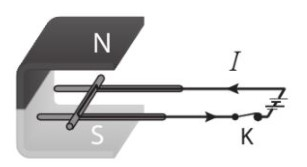
\includegraphics[width=0.3\linewidth]{figs/VN12-Y24-PH-SYL-018P-8}
	\end{center}
	\begin{enumerate}[label=\alph*)]
		\item Thanh kim loại sẽ lăn theo hướng nào khi đóng công tắc K?
		\item Nêu cách làm cho thanh kim loại lăn theo hướng ngược lại.
	\end{enumerate}
	\loigiai{
		\begin{enumerate}[label=\alph*)]
			\item Thanh kim loại dẫn điện sẽ lăn về bên phải.
			\item Đảo ngược chiều dòng điện hoặc đổi chiều của từ trường.
		\end{enumerate}	
	}
\end{ex}

% ===================================================================
\begin{ex}
	Xác định hướng của lực từ tác dụng lên các đoạn dây dẫn có dòng điện chạy qua, được đặt trong từ trường đều như các hình dưới đây:
	\begin{center}
		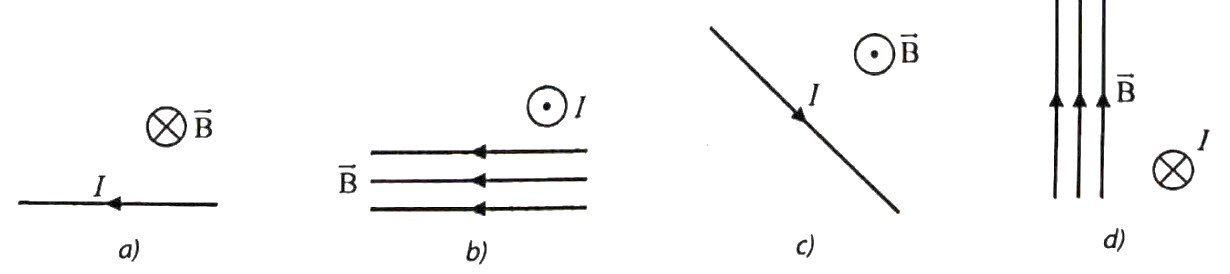
\includegraphics[width=0.8\linewidth]{figs/VN12-Y24-PH-SYL-018P-3}
	\end{center}
	\loigiai{
		\begin{center}
			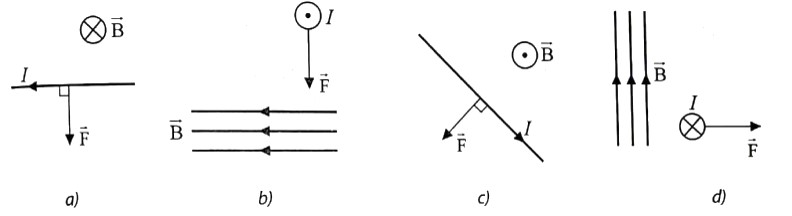
\includegraphics[width=0.8\linewidth]{figs/VN12-Y24-PH-SYL-018P-4}
		\end{center}	
	}
\end{ex}
% ======================================================================
\begin{ex}
	Xác định phương và chiều lực từ tác dụng lên các cạnh của khung. Biết chiều của vector cảm ứng từ $\vec{B}$ và chiều dòng điện được cho như mỗi hình vẽ.
	\begin{center}
		\begin{tabular}{cc}
			\begin{tikzpicture}
				\coordinate (A) at(0,0);
				\coordinate (B) at(0,-3);
				\coordinate (C) at(4,-3);
				\coordinate (D) at(0.5,0);
				\draw[decoration={markings, mark=at position 0.5 with{\arrow{stealth}}}, postaction={decorate}, line width=1.5pt](A)--(B)--(C)--(D);
				\foreach \y in {-0.5,-1.5,-2.5}{
					\draw[-latex, blue, line width=1.5pt] (-1,\y) --(4.5,\y);	
					\node[blue] at(4.5,0) {$\vec{B}$};
				}
				\node[left] at(A) {A};
				\node[left] at(B) {B};
				\node[right] at(C) {C};
				\node[above right] at(D) {D};
			\end{tikzpicture}
			&
			\begin{tikzpicture}
				\coordinate (A) at(0,0);
				\coordinate (B) at(0,-3);
				\coordinate (C) at(4,-3);
				\coordinate (D) at(4,0);
				\coordinate (E) at(0.5,0);
				\draw[decoration={markings, mark=at position 0.35 with{\arrow{stealth}}}, postaction={decorate}, line width=1.5pt](A)--(B)--(C)--(D)--(E);
				
				\node[left] at(A) {A};
				\node[left] at(B) {B};
				\node[right] at(C) {C};
				\node[right] at(D) {D};
				\node[above] at(E) {E};
				\node[blue] at(2,-1.5) {\LARGE $\odot$};
				\node[blue, right] at(2.2,-1.5) {$\vec{B}$};
			\end{tikzpicture}\\
			Hình a & Hình b
		\end{tabular}
	\end{center}
	\loigiai{
		\begin{center}
			\begin{tabular}{M{6cm}M{6cm}}
				\begin{tikzpicture}
					\coordinate (A) at(0,0);
					\coordinate (B) at(0,-3);
					\coordinate (C) at(4,-3);
					\coordinate (D) at(0.5,0);
					\draw[decoration={markings, mark=at position 0.5 with{\arrow{stealth}}}, postaction={decorate}, line width=1.5pt](A)--(B)--(C)--(D);
					\foreach \y in {-0.5,-1.5,-2.5}{
						\draw[-latex, blue, line width=1.5pt] (-1,\y) --(4.5,\y);	
						\node[blue] at(4.5,0) {$\vec{B}$};
					}
					\node[left] at(A) {A};
					\node[left] at(B) {B};
					\node[right] at(C) {C};
					\node[above right] at(D) {D};
					\node[red, fill=white, minimum size=0pt,inner sep=0pt, circle] at (0,-1.5) {\LARGE$\odot$};
					\node[red, below right] at (0.25,-1.5) {$\vec{F}_{\text{AB}}$};
					\node[red, fill=white, minimum size=0pt,inner sep=0pt, circle] at ($(D)!0.5!(C)$) {\LARGE$\otimes$};
					\node[red, below] at ($(D)!0.5!(C)+(0,-0.25)$) {$\vec{F}_{\text{CD}}$};
				\end{tikzpicture}
				&
				\begin{tikzpicture}
					\coordinate (A) at(0,0);
					\coordinate (B) at(0,-3);
					\coordinate (C) at(4,-3);
					\coordinate (D) at(4,0);
					\coordinate (E) at(0.5,0);
					\draw[decoration={markings, mark=at position 0.35 with{\arrow{stealth}}}, postaction={decorate}, line width=1.5pt](A)--(B)--(C)--(D)--(E);
					\draw[-latex, red, line width=1.5pt] ($(A)!0.5!(B)$)--+(-1,0);
					\draw[-latex, red, line width=1.5pt] ($(B)!0.5!(C)$)--+(0,-1);
					\draw[-latex, red, line width=1.5pt] ($(C)!0.5!(D)$)--+(1,0);
					\draw[-latex, red, line width=1.5pt] ($(D)!0.5!(E)$)--+(0,1);
					\node[left] at(A) {A};
					\node[left] at(B) {B};
					\node[right] at(C) {C};
					\node[right] at(D) {D};
					\node[above] at(E) {E};
					\node[blue] at(2,-1.5) {\LARGE $\odot$};
					\node[blue, right] at(2.2,-1.5) {$\vec{B}$};
					\node[red, above] at ($(A)!0.5!(B)+(-1,0)$) {$\vec{F}_{\text{AB}}$};
					\node[red, right] at ($(B)!0.5!(C)+(0,-1)$) {$\vec{F}_{\text{BC}}$};
					\node[red, above] at ($(C)!0.5!(D)+(1,0)$) {$\vec{F}_{\text{CD}}$};
					\node[red, right] at ($(D)!0.5!(E)+(0,1)$) {$\vec{F}_{\text{DE}}$};
				\end{tikzpicture}\\
				Hình a & Hình b
			\end{tabular}
		\end{center}	
	}
\end{ex}



% ===================================================================
\begin{ex}
	\immini{Động cơ điện là thiết bị có thể chuyển hoá năng lượng điện thành cơ năng (chuyển động quay của động cơ). Mô hình đơn giản của một động cơ điện gồm: một khung dây dẫn hình chữ nhật ABCD đang có dòng điện không đổi chạy qua. Khung dây được đặt vào trong từ trường đều có các đường sức từ thẳng đứng như hình bên. Tại thời điểm ban đầu, khung đang ở vị trí sao cho hai cạnh AB và CD đang song song với các đường sức từ. Vẽ các lực từ tác dụng lên các cạnh của khung dây. Các lực này có tác dụng làm cho khung dây chuyển động như thế nào?	}
	{
		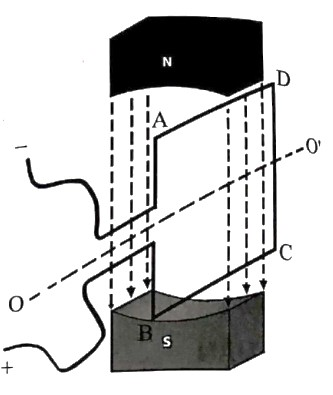
\includegraphics[width=0.45\linewidth]{figs/VN12-Y24-PH-SYL-018P-5}
	}
	\loigiai{
		Chỉ có lực từ tác dụng lên hai cạnh AD và BC của khung dây. Hai lực này tạo ra cặp ngẫu lực và có tác dụng tạo ra moment ngẫu lực làm quay khung dây.
		\begin{center}
			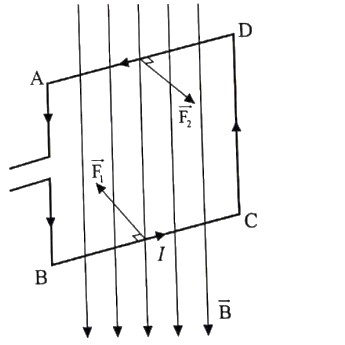
\includegraphics[width=0.4\linewidth]{figs/VN12-Y24-PH-SYL-018P-6}
		\end{center}	
	}
\end{ex}

% =================================================================
\begin{ex}
	Cho hai dây dẫn thẳng song song, dài vô hạn lần lượt có dòng điện $I_1$ và $I_2$ chạy qua như hình \ref{fig:17P-1}. Xét mặt phẳng $\left(Oxy\right)$ vuông góc với cả hai dòng điện, cắt các dòng điện tại A và B.
	\begin{center}
		\begin{tikzpicture}
			\coordinate (O) at (0,0);
			\coordinate (A) at ($(O)+(75:3)$);
			\coordinate (C) at (6,0);
			\coordinate (B) at ($(C)+(75:3)$);
			\fill[orange!50!white, opacity=0.6] (O)--(A)--(B)--(C)--(O);
			\draw[-latex, line width=1.5pt] (O)--+(75:4);
			\draw[-latex, line width=1.5pt] (O)--+(7,0);
			\draw[line width=1pt, dashed] (1,1.45)--(6,1.45);
			\draw[line width=1.5pt, blue,decoration={markings, mark=at position 0.625 with {\arrow{stealth}}},
			postaction={decorate}] 
			(1.5,1.45)--+(0,2.5);
			\draw[line width=1.5pt, blue, dashed] (1.5,1.45)--+(0,-1.45);
			\draw[line width=1.5pt, blue] (1.5,0)--+(0,-1);
			\draw[line width=1.5pt, blue,decoration={markings, mark=at position 0.625 with {\arrow{stealth}}},
			postaction={decorate}] 
			(3.5,1.45)--+(0,2.5);
			\draw[line width=1.5pt, blue, dashed] (3.5,1.45)--+(0,-1.45);
			\draw[line width=1.5pt, blue] (3.5,0)--+(0,-1);
			\filldraw (1.5,1.45) circle(2pt) node[above left] {A};
			\filldraw (3.5,1.45) circle(2pt) node[above left] {B};
			\filldraw (5,1.45) circle(2pt) node[above left] {C};
			\node[left] at (O) {O};
			\node[below] at (7,0) {$x$};
			\node[left] at ($(O)+(75:4)$) {$y$};
			\node[right] at (1.5,3) {$I_1$};
			\node[right] at (3.5,3) {$I_2$};
		\end{tikzpicture}
	\end{center}
	\captionof{figure}{}
	\label{fig:17P-1}
	\begin{enumerate}[label=\alph*)]
		\item Xác định phương, chiều của các vector cảm ứng từ do từng dòng điện gây ra tại C (A, B, C thẳng hàng).
		\item Nếu đặt một kim la bàn tại điểm C thì kim la bàn này sẽ định hướng như thế nào? Giải thích.
	\end{enumerate}
	\loigiai{\begin{enumerate}[label=\alph*)]
			\item Dựa vào quy tắc nắm tay phải, ta xác định được vector cảm ứng từ do hai dòng điện $I_1$ và $I_2$ gây ra tại điểm C đều nằm trong mặt phẳng $\left(Oxy\right)$, phương song song và cùng chiều với trục $Oy$.
			\item Hai vector cảm ứng từ do hai dòng điện $I_1$ và $I_2$ gây ra đều cùng hướng với nhau nên kim la bàn khi đặt tại C sẽ có cực Bắc hướng theo chiều dương trục $Oy$ còn cực Nam hướng ngược lại.
	\end{enumerate}}
\end{ex}
% ===================================================================
\begin{ex}
	Một dây dẫn có chiều dài $L=\SI{1.2}{\meter}$, được đặt trong từ trường đều có độ lớn $B=\SI{5E-2}{\tesla}$. Cường độ dòng điện chạy trong dây dẫn có giá trị $\SI{3}{\ampere}$. Hãy xác định độ lớn của lực từ tác dụng lên dây dẫn trong các trường hợp sau đây:
	\begin{enumerate}[label=\alph*)]
		\item Dây dẫn đặt vuông góc với các đường sức từ.
		\item Dây dẫn đặt song song với các đường sức từ.
		\item Dây dẫn hợp với các đường sức từ một góc $\SI{45}{\degree}$.
	\end{enumerate}	
	\loigiai{
		\begin{enumerate}[label=\alph*)]
			\item $F=ILB\sin\SI{90}{\degree}=\SI{0.18}{\newton}$.
			\item $F=ILB\sin\SI{0}{\degree}=\SI{0}{\newton}$.
			\item $F=ILB\sin\SI{45}{\degree}\approx\SI{0.13}{\newton}$.
		\end{enumerate}	
	}
\end{ex}
% ===================================================================
\begin{ex}
	Một đoạn dây dẫn thẳng dài $\SI{20}{\centi\meter}$ mang dòng điện có cường độ $\SI{50}{\milli\ampere}$ được đặt vào một vùng từ trường đều có cảm ứng từ $\SI{100}{\micro\tesla}$. Xác định góc hợp bởi đoạn dây và vector cảm ứng từ để lực từ tác dụng lên đoạn dây đạt độ lớn cực đại. Tính giá trị cực đại này.	
	\loigiai{
		Từ biểu thức tính độ lớn lực từ $F=B I L \sin \theta$, ta thấy lực từ đạt độ lớn cực đại khi: $\sin \theta=1 \Rightarrow \theta=\SI{90}{\degree}$. Khi đó, $F=B I L=100 \cdot 10^{-6} \cdot 50 \cdot 10^{-3} \cdot 0,2=\SI{E-6}{\newton}$.
		
	}
\end{ex}

% ===================================================================
\begin{ex}
	Một đoạn dây dẫn dài $\SI{5}{\centi\meter}$ đặt trong từ trường đều và vuông góc với vector cảm ứng từ. Dòng điện chạy qua dây có cường độ $\SI{0.75}{\ampere}$. Lực từ tác dụng lên đoạn dây đó là $\SI{3E-2}{\newton}$. Tính độ lớn cảm ứng từ.
	\loigiai{
		$$
		B=\frac{F}{IL\sin \theta}=\frac{3 \cdot 10^{-2}}{0,75 \cdot 0,05 \cdot \sin \SI{90}{\degree}}=\SI{0.8}{\tesla}.
		$$	
	}
\end{ex}
% ===================================================================
\begin{ex}
	Một đoạn dây dẫn dài $\SI{10}{\centi\meter}$ đặt trong từ trường đều, hợp với vector cảm ứng từ một góc $\SI{30}{\degree}$. Dòng điện có cường độ $\SI{2}{\ampere}$ chạy qua dây dẫn thì lực từ tác dụng lên đoạn dây có độ lớn là $\SI{4E-2}{\newton}$. Tính độ lớn của cảm ứng từ.
	\loigiai{
		Ta có: $\alpha=\SI{30}{\degree} \Rightarrow \sin \theta=\frac{1}{2}$. \\
		Cảm ứng từ của từ trường có độ lớn: $B=\dfrac{F}{IL\sin \theta}=\dfrac{4 \cdot 10^{-3}}{2 \cdot 0,1 \cdot 0,5}=\SI{0.04}{\tesla}$.	
	}
\end{ex}
% ===================================================================
\begin{ex}
	Một đoạn dây dẫn thẳng MN có chiều dài $\SI{6}{\centi\meter}$, có cường độ dòng điện $I=\SI{5}{\ampere}$ chạy qua đặt trong từ trường đều có cảm ứng từ $B=\SI{0.5}{\tesla}$. Lực từ tác dụng lên đoạn dây có độ lớn $F=\SI{7.5E-2}{\newton}$. Tính góc $\theta$ hợp bởi dây MN và vector cảm ứng từ.	
	\loigiai{
		Độ lớn của lực từ tác dụng lên đoạn dây dẫn có chiều dài $L$ mang dòng điện $I$ đặt trong từ trường cảm ứng từ $B$ là: $F=ILB \sin\theta \Rightarrow \sin\theta=0,5 \Rightarrow \theta=\SI{30}{\degree}.$	
	}
\end{ex}
% ===================================================================
\begin{ex}
	Một đoạn dây dài $L$ đặt trong từ trường đều có cảm ứng từ $B=\SI{0.5}{\tesla}$ hợp với đường cảm ứng từ một góc $\SI{30}{\degree}$. Dòng điện qua dây có cường độ $\SI{0.5}{\ampere}$, thì lực từ tác dụng lên đoạn dây là $\SI{4E-2}{\newton}$. Tính chiều dài đoạn dây dẫn.	
	\loigiai{
		Chiều dài đoạn dây dẫn:
		$$
		L=\frac{F}{IB \sin \theta}=\frac{4 \cdot 10^{-2}}{0,5 \cdot 0,5 \cdot \sin \SI{30}{\degree}}=\SI{0.32}{\meter}=\SI{32}{\centi\meter}.
		$$
		
	}
\end{ex}
% ===================================================================
\begin{ex}
	Một đoạn dây dẫn dài $L=\SI{0.5}{\meter}$ đặt trong từ trường đều sao cho dây dẫn hợp với vector cảm ứng từ một góc $\SI{45}{\degree}$. Biết cảm ứng từ $B=\SI{0.2}{\tesla}$ và dây dẫn chịu lực từ $F=\SI{4E-2}{\newton}$. Tính cường độ dòng điện chạy qua dây dẫn.
	\loigiai{
		$$
		I=\frac{F}{BL \sin \theta}=\frac{4 \cdot 10^{-2}}{0,2 \cdot 0,5 \cdot \sin \SI{45}{\degree}}=\xsi{0,4\sqrt{2}}{\ampere}.
		$$
		
	}
\end{ex}
% ===================================================================
\begin{ex}
	Một đường dây tải điện thẳng dài $\SI{42}{\meter}$ có dòng điện với cường độ $\SI{150}{\ampere}$ chạy qua theo hướng về phía Bắc. Từ trường Trái Đất tại vị trí này có độ lớn khoảng $\SI{0.5E-4}{\tesla}$, có hướng lệch một góc $\theta=\SI{50}{\degree}$ so với dòng điện. Xác định lực từ tác dụng lên đường dây nói trên.
	\begin{center}
		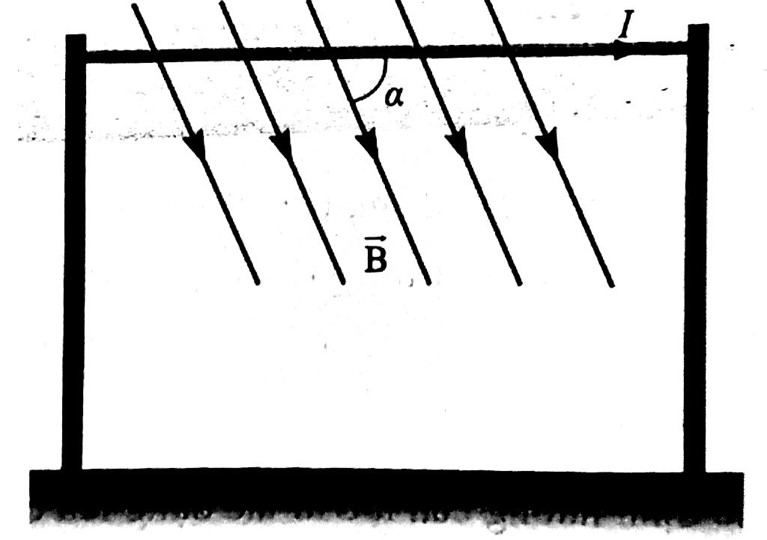
\includegraphics[width=0.4\linewidth]{figs/VN12-Y24-PH-SYL-018P-7}
	\end{center}
	\loigiai{
		Lực từ tác dụng lên đường dây có chiều hướng về phía Tây và có độ lớn là:
		$$F=B I L \sin \theta=0,5 \cdot 10^{-4} \cdot 150 \cdot 42 \cdot \sin \SI{50}{\degree} \approx \SI{0.24}{\newton}.$$
		
	}
\end{ex}
% ======================================================================
\begin{ex}
	Một dây dẫn có dòng điện $\SI{22.0}{\ampere}$ chạy từ Tây sang Đông. Giả sử tại vị trí này, từ trường Trái Đất nằm ngang và hướng từ Nam lên Bắc với độ lớn $\SI{0.5E-4}{\tesla}$.
	\begin{enumerate}[label=\alph*)]
		\item Tìm độ lớn và hướng của lực từ tác dụng lên một đoạn dây dài $\SI{36.0}{\meter}$.
		\item Tính lực hấp dẫn tác dụng lên đoạn dây có cùng chiều dài nếu nó được làm bằng đồng và có diện tích mặt cắt ngang là $\SI{2.50E-6}{\meter^2}$. Khối lượng riêng của đồng là $\SI{8.9E3}{\kilogram/\meter^3}$, lấy $g=\SI{9.80}{\meter/\second^2}$.
	\end{enumerate}
	\loigiai{
		\begin{enumerate}[label=\alph*)]
			\item $F_{\text{từ}}=ILB=\SI{3.96E-2}{\newton}$, hướng vuông góc với trang giấy, từ sau ra trước.
			\item $F_{\text{hấp dẫn}}=\rho gLS=\SI{7.85}{\newton}$.
			
		\end{enumerate}	
	}
\end{ex}
% ======================================================================
\begin{ex}
	Một dây dẫn thẳng, cứng, dài $\SI{20}{\centi\meter}$, có khối lượng $\SI{50}{\gram}$ được giữ nằm yên theo phương ngang trong một từ trường có độ lớn cảm ứng từ là $\SI{0.49}{\tesla}$ và có hướng nằm ngang, vuông góc với dây. Cường độ dòng điện chạy trong dây là bao nhiêu để khi dây được thả ra thì nó vẫn nằm yên? Lấy $g=\SI{9.8}{\meter/\second^2}$.
	
	\loigiai{
		$$F_{\text{từ}}	=P\Leftrightarrow ILB=mg\Rightarrow I=\dfrac{mg}{BL}=\SI{5.0}{\ampere}.$$
	}
\end{ex}

% ===================================================================
\begin{ex}
	Treo một đoạn dây dẫn có chiều dài $L=\SI{5}{\centi\meter}$, khối lượng $m=\SI{5}{\gram}$ bằng hai dây mảnh, nhẹ sao cho dây dẫn nằm ngang. Biết cảm ứng từ của từ trường hướng thẳng đứng xuống dưới, có độ lớn $B=\SI{0.5}{\tesla}$ và dòng điện chạy qua dây dẫn là $I=\SI{2}{\ampere}$. Lấy $g=\SI{10}{\meter/\second^2}$. Tính góc lệch của dây treo so với phương thẳng đứng.
	\loigiai{
		$$
		\tan \theta=\frac{F_t}{P}=\frac{0,5 \cdot 2 \cdot 0,05}{0,005 \cdot 10}=1 \Rightarrow \theta=\SI{45}{\degree}.
		$$
		
	}
\end{ex}
% ===================================================================
\begin{ex}
	Một đoạn dây dẫn thẳng MN có chiều dài $L=\SI{6}{\centi\meter}$, có dòng điện cường độ $I=\SI{5}{\ampere}$ chạy qua đặt trong từ trường đều có cảm ứng từ $B=\SI{0.5}{\tesla}$. Lực từ tác dụng lên đoạn dây có độ lớn $F=\SI{7.5E-2}{\newton}$. Tính góc $\theta$ hợp bởi dây MN và vector cảm ứng từ.
	\loigiai{
		Áp dụng công thức $F=ILB \sin \theta$ với $L=\SI{6E-2}{\meter}, I=\SI{5}{\ampere}, F=\SI{7.5E-2}{\newton}$ và $B=\SI{0.5}{\tesla}$, ta tính được $\theta=\SI{30}{\degree}$.
		
	}
\end{ex}
% ======================================================================
\begin{ex}
	Thanh MN dài $\ell=\SI{20}{\centi\meter}$ có khối lượng $\SI{5}{\gram}$ treo nằm ngang bằng hai sợi chỉ mảnh CM và DN. Thanh nằm trong từ trường đều có cảm ứng từ	 $B=\SI{0.3}{\tesla}$ nằm ngang vuông góc với thanh có chiều như hình vẽ. Mỗi sợi chỉ treo thanh có thể chịu được lực kéo tối đa là $\SI{0.04}{\newton}$. Dòng điện chạy qua thanh MN có chiều và cường độ lớn nhất là bao nhiêu thì sợi chỉ treo thanh chưa bị đứt. Lấy gia tốc trọng trường $g=\SI{9.8}{\meter/\second^2}$.
	\begin{center}
		\begin{tikzpicture}
			\coordinate (C) at (0,0);
			\coordinate (D) at (4,0);
			\coordinate (M) at (0,-3);
			\coordinate (N) at (4,-3);
			\draw[line width=1pt] (C)--+(-0.5,0)--+(4.5,0);
			\draw[line width=1pt] (C)--(M);
			\draw[line width=1pt] (D)--(N);
			\draw[line width=3pt] (M)--(N);
			\node[blue] at (2,-1.5) {\LARGE$\otimes$};
			\node[blue, right] at (2.25,-1.5) {$\vec{B}$};
			\node[above] at (C) {C};
			\node[above] at (D) {D};
			\node[left] at (M) {M};
			\node[right] at (N) {N};
		\end{tikzpicture}
	\end{center}
	\loigiai{
		Khi cho dòng điện chạy qua dây dẫn đặt trong từ trường thì sẽ có lực từ tác dụng lên dây dẫn.
		\begin{itemize}
			\item Công thức tính lực từ: $F=IB \ell \sin \alpha$.
			\item Dây bị đứt khi lực từ hướng xuống.\\
			Để dây không đứt thì $P+F \leq 2 T \Rightarrow F \leq 2T-P$
			$$
			\begin{aligned}
				& \Rightarrow F_{\text{max}}=BI_{\text{max}} \ell \sin \SI{90}{\degree}=2T-mg \\
				& \Rightarrow I_{\text{max}}=\frac{2 T-mg}{B\ell} \\
				& \Rightarrow I_{\text{max}}=\frac{2 \cdot 0,04-0,005 \cdot 9,8}{0,3 \cdot 0,2}\approx \SI{0.52}{\ampere}.
			\end{aligned}
			$$
		\end{itemize}
		Xác định chiều của dòng điện bằng cách sử dụng quy tắc bàn tay trái. Để lực từ hướng xuống thì dòng điện phải có chiều từ N đến M.	
	}
\end{ex}



% ======================================================================
\begin{ex}
	Một dây dẫn được gập thành khung dây dạng tam giác vuông cân MNP với $\mathrm{MN}=\mathrm{NP}=\SI{10}{\centi\meter}$. Đặt khung dây vào từ trường $B=\SI{E-2}{\tesla}$ có chiều như hình vẽ. Cho dòng điện có cường độ $I=\SI{10}{\ampere}$ vào khung theo chiều MNPM. Lực từ tác dụng vào các cạnh của khung dây là bao nhiêu?
	\begin{center}
		\begin{tikzpicture}
			\coordinate (M) at(0,0);
			\coordinate (N) at(0,-3);
			\coordinate (P) at(3,-3);
			\coordinate (Q) at(0.25,0);
			\draw[line width=1.5pt] (M)--(N)--(P)--(Q);
			\foreach \y in {-0.5,-1.5,-2.5}{
				\draw[-latex, blue, line width=1.5pt] (-0.5,\y)--(3.5,\y);	
			}
			\node[left] at(M) {M};
			\node[left] at(N) {N};
			\node[right] at(P) {P};
			\node[blue,right] at (3.5,-1.5) {$\vec{B}$};
		\end{tikzpicture}
	\end{center}
	\loigiai{
		\begin{itemize}
			\item Vì MN vuông với $\vec{B}$ nên:
			$$F_\mathrm{MN}=BIL\sin\SI{90}{\degree}=\SI{E-2}{\newton}.$$
			\item Vì NP song song với $\vec{B}$ nên:
			$$
			F_\mathrm{NP}=B I L \sin \SI{0}{\degree}=0
			$$
			\item  Từ hình ta thấy $\overrightarrow{PM}$ tạo với $\vec{B}$ một góc:
			$$
			\alpha=180-45=\SI{135}{\degree}
			$$
			Do đó lực tác dụng lên đoạn PM là:
			$$
			F_\mathrm{PM}=B I L \sin \SI{135}{\degree}=\SI{E-2}{\newton}.
			$$
		\end{itemize}	
	}
\end{ex}
% ======================================================================
\begin{ex}
	Trong giờ thực hành đo độ lớn cảm ứng từ bằng "cân dòng điện" với bố trí thí nghiệm được thể hiện như trong hình 11.1 (dụng cụ thí nghiệm và các bước tiến hành thí nghiệm lần lượt được trình bày ở Bài 10 và Bài 11 trong SGK), một bạn học sinh đã thu được bảng số liệu như bảng dưới đây. Hãy xử lí số liệu thu được để đưa ra kết quả độ lớn cảm ứng từ trong thí nghiệm này.
	\begin{center}
		\begin{tabular}{|M{2cm}|M{2cm}|M{2cm}|M{2cm}|M{4cm}|M{3.5cm}|}
			\hline
			\multicolumn{6}{|M{17cm}|}{$\theta=\SI{90}{\degree}$; $L=\SI{0.04}{\meter}$; $N=\SI{200}{\text{vòng}}$}\\
			\hline
			\thead{Lần đo} & $\xsi{I}{\left(\ampere\right)}$ & $\xsi{F_1}{\left(\newton\right)}$ & $\xsi{F_2}{\left(\newton\right)}$ & $F=\xsi{F_2-F_1}{\left(\newton\right)}$ & $B=\xsi{\frac{F}{NIL}}{\left(\tesla\right)}$\\
			\hline
			1 & 0,4 & 0,210 & 0,320 &&\\
			\hline
			2 & 0,8 & 0,220 & 0,440 & &\\
			\hline
			3 & 1,0 & 0,200 & 0,480 & &\\
			\hline
			\multicolumn{5}{|M{12cm}|}{\thead{Trung bình}} &$\overline{B}=$\\
			\hline
			
		\end{tabular}
	\end{center}	
	\loigiai{
		\begin{center}
			\begin{tabular}{|M{2cm}|M{2cm}|M{2cm}|M{2cm}|M{4cm}|M{3.5cm}|}
				\hline
				\multicolumn{6}{|M{17cm}|}{$\theta=\SI{90}{\degree}$; $L=\SI{0.04}{\meter}$; $N=\SI{200}{\text{vòng}}$}\\
				\hline
				\thead{Lần đo} & $\xsi{I}{\left(\ampere\right)}$ & $\xsi{F_1}{\left(\newton\right)}$ & $\xsi{F_2}{\left(\newton\right)}$ & $F=\xsi{F_2-F_1}{\left(\newton\right)}$ & $B=\xsi{\frac{F}{NIL}}{\left(\tesla\right)}$\\
				\hline
				1 & 0,4 & 0,210 & 0,320 &0,110&0,034\\
				\hline
				2 & 0,8 & 0,220 & 0,440 &0,220 &0,034\\
				\hline
				3 & 1,0 & 0,200 & 0,480 &0,280 &0,035\\
				\hline
				\multicolumn{5}{|M{12cm}|}{\thead{Trung bình}} &$\overline{B}=0,0343$\\
				\hline
				
			\end{tabular}
		\end{center}		
	}
\end{ex}

% ======================================================================
\begin{ex}
	Sơ đồ bố trí thí nghiệm dưới đây được sử dụng để xác định độ lớn cảm ứng từ $B$ giữa các cực của nam châm.\\
	Nam châm được đặt trên cân. Dây dẫn mang dòng điện được đặt cố định nằm ngang và vuông góc với từ trường giữa các cực của nam châm. Lấy gia tốc rơi tự do $g=\SI{9.8}{\meter/\second^2}$.
	\begin{center}
		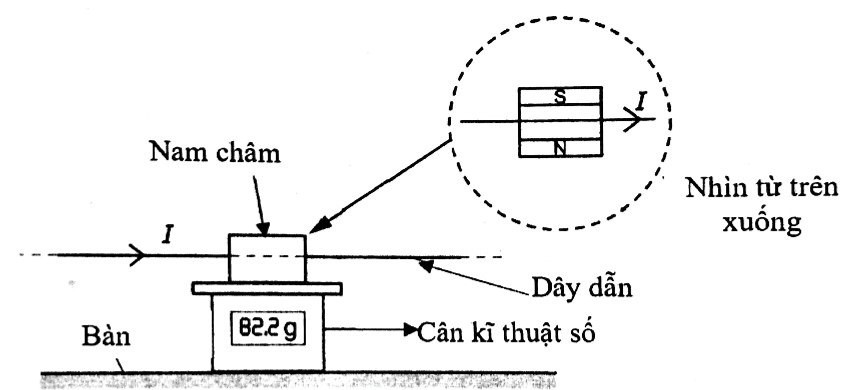
\includegraphics[width=0.6\linewidth]{figs/VN12-Y24-PH-SYL-018P-9}
	\end{center}
	Số liệu thu thập được như sau:
	\begin{itemize}
		\item Chiều dài của dây trong từ trường đều của nam châm: $\ell=\xsi{6,0\pm 0,2}{\centi\meter}$;
		\item Số chỉ của cân khi không có dòng điện trong dây dẫn: $\SI{80,0}{\gram}$;
		\item Số chỉ của cân khi có dòng điện trong dây: $\SI{82.2}{\gram}$;
		\item Dòng điện trong dây: $I=\xsi{5,0\pm0,1}{\ampere}$.
	\end{itemize}
	Viết kết quả đo giá trị của $B$. Bỏ qua sai số của cân.
	\loigiai{
		Dây dẫn đặt trong từ trường nam châm nên chịu tác dụng lực từ $F$.\\
		Lực $F$ hướng xuống tác dụng lên cân giống như một trọng lực $\mathrm{P}=\mathrm{mg}$.
		Với $m$ là chênh lệch số chỉ đọc ở cân khi có và không có dòng điện trong dây:
		$$
		\begin{aligned}
			& m=82,2-80,0=\SI{2.2}{\gram} \\
			& F=m g=2,2 \cdot 10^{-3} \cdot 9,8=\SI{0.0216}{\newton} \\
			& B=\frac{F}{I \ell \sin \alpha}=\frac{0,0216}{5,0.0,06 \cdot \sin \SI{90}{\degree}}\approx\SI{0.072}{\tesla}
		\end{aligned}
		$$
		
		Bỏ qua sai số của $F$ thì:
		$$
		\frac{\Delta B}{B}=\frac{\Delta I}{I}+\frac{\Delta \ell}{\ell} \Leftrightarrow \frac{\Delta B}{0,072}=\frac{0,1}{5}+\frac{0,2}{6} \Rightarrow \Delta B\approx0,004 T
		$$
		
		Kết quả đo: $B=\overline{B} \pm \Delta B=0,072 \pm \SI{0.004}{\tesla}$	
	}
\end{ex}
%	\NOTE
	%==================Mục lục chính

\end{document}

